%%
%% This is file `thesis-ex.tex',
%% generated with the docstrip utility.
%%
%% The original source files were:
%%
%% uiucthesis2009.dtx  (with options: `example')
%% 
\def\fileversion{v2.25a} \def\filedate{2009/10/10}
%% Package and Class "uiucthesis2009" for use with LaTeX2e.
\documentclass[edeposit,fullpage]{uiucthesis2009}
\usepackage[usenames, dvipsnames]{color}
\usepackage{graphicx}
\usepackage{xspace}     %to get spaces in commands right
\usepackage{subfig}
\usepackage{url}
\usepackage{booktabs}
\usepackage{enumitem}
\usepackage{wrapfig}
\usepackage{lipsum}
\usepackage{caption}
\usepackage{multirow}
\usepackage{longtable}
\usepackage{amsmath}
\usepackage{rotating}
\usepackage{amssymb}
\usepackage{colortbl}
\usepackage{xcolor}
\usepackage{units}      %to get proper nobreak spaces for units
\usepackage{hyperref}   %clickable links in pdfs

\nocopyrightpage

\newcolumntype{L}{>{\hspace*{-\tabcolsep}}c}
\newcolumntype{R}{c<{\hspace*{-\tabcolsep}}}
\newcommand{\ra}[1]{\renewcommand{\arraystretch}{#1}}
\colorlet{tableheadcolor}{gray!25} % Table header colour = 25% gray
\newcommand{\headcol}{\rowcolor{tableheadcolor}} %
\colorlet{tablerowcolor}{gray!10} % Table row separator colour = 10% gray
\newcommand{\rowcol}{\rowcolor{tablerowcolor}}

\newcommand{\CN}{\textcolor{red}{$^{[citation\ needed]}$}}
\newcommand{\Jpsi}{J/\Psi}
\newcommand{\us}{$\mu$s\xspace}
\newcommand{\red}[1]{\emph{\textcolor{red}{#1}}}
\newcommand{\bigoh}{\mathcal{O}}
\newcommand{\dbar}{\bar{d}}
\newcommand{\ubar}{\bar{u}}
\newcommand{\sbar}{\bar{s}}
\newcommand{\cbar}{\bar{c}}

\begin{document}

\title{Nuclear dependence of proton-induced Drell-Yan dimuon production at \unit[120]{GeV} at SeaQuest}
\author{Bryan P. Dannowitz}
\department{Nuclear Physics}
\schools{B.S., New Mexico Institute of Mining and Technology, 2008}
\phdthesis
\advisor{Naomi C. R. Makins}
\degreeyear{2016}
\committee{Professor Jen-Chieh Peng, Chair\\
	Professor Naomi C. R. Makins, Director of Research\\
	Professor Michael Stone\\
	Professor Jim Eckstein}
\maketitle

\frontmatter

%% Create an abstract that can also be used for the ProQuest abstract.
%% Note that ProQuest truncates their abstracts at 350 words.
\begin{abstract}
A measurement of the atomic mass ($A$) dependence of $p+A\rightarrow\mu^+\mu^- + X$ Drell-Yan dimuons produced by \unit[120]{GeV} protons is presented here. The data was taken by the SeaQuest experiment at Fermilab using a proton beam extracted from its Main Injector. Over 88,000 dimuon pairs were recorded with invariant mass $4.2 < M_{\gamma^*} < \unit[10] GeV$ and target parton momentum fraction $0.1\leq x_2 \leq 0.5$ for nuclear targets $^1H,\ ^2H,\ C,\ Fe,\ $and$\ W$. The ratio of dimuon yields per nucleon ($Y$) for heavy nuclei versus $^2H$, $R^{DY} = Y^{(A)} / Y^{(^2H)} \approx \bar{q}_u^{(A)}(x)/\bar{q}_u^{(^2H)}(x)$, is sensitive to modifications in the anti-quark sea distributions ($\bar{q}(x)$) in nuclei for the case of proton-induced Drell-Yan. The data analyzed here provides tighter constraints on various models that attempt to define the anomalous behavior of nuclear modification as seen in deep inelastic lepton scattering, a phenomenon better known as the EMC effect.

\end{abstract}

%% Create a dedication in italics with no heading, centered vertically
%% on the page.

\begin{dedication}
Dedicated to my grandfather, Ted, who took me to school every day.
\end{dedication}

%% Create an Acknowledgements page, many departments require you to
%% include funding support in this.
\chapter*{Acknowledgments}

\red{Don't forget to acknowledge the NSF and mention the grant number!}

%% The thesis format requires the Table of Contents to come
%% before any other major sections, all of these sections after
%% the Table of Contents must be listed therein (i.e., use \chapter,
%% not \chapter*).  Common sections to have between the Table of
%% Contents and the main text are:
%%
%% List of Tables
%% List of Figures
%% List Symbols and/or Abbreviations
%% etc.

\tableofcontents
\listoftables
\listoffigures

%% Create a List of Abbreviations. The left column
%% is 1 inch wide and left-justified
\chapter{List of Abbreviations}

\begin{symbollist*}
	\item[ACNET] Accelerator control system network
	\item[AD] Accelerator division (of Fermilab)
	\item[BIM] Beam intensity monitor
	\item[BNC] Bayonet Neill–Concelman signal cable connector standard
	\item[BOS] Beginning of spill
	\item[BPM] Beam profile monitor
	\item[CEBAF] Continuous Electron Beam Accelerator Facility
	\item[CODA] CEBAF On-line Data Acquisition
	\item[CS] Collins-Soper reference frame
	\item[CTEQ] Coordinated theoretical-experimental project on QCD
	\item[DAQ] Data acquisition
	\item[DC] Drift chamber
	\item[DIS] Deep-inelastic scattering
	\item[DY] Drell-Yan
	\item[EOS] End of spill
	\item[EOF] End of file
	\item[EPICS] Experimental physics and industrial control system
	\item[EVIO] CODA event input/output
	\item[FEE] Front-end electronics
	\item[FNAL] Fermi National Accelerator Laboratory (Fermilab)
	\item[FPGA] Field programmable gate arrays
	\item[IC] Ion chamber
	\item[LED] Light-emitting diode
	\item[LINAC] Fermilab Linear Accelerator
	\item[LO] Leading order
	\item[MI] (Fermilab) Main Injector
	\item[MOSFET] Metal–oxide–semiconductor field-effect transistor
	\item[NDF] Neutral density filter
	\item[NLO] Next-to-leading order
	\item[NM] Neutrino-muon beam line
	\item[NNLO] Next-to-next-to-leading order
	\item[PCB] Printed circuit board
	\item[PDF] Parton distribution function
	\item[PID] Particle identification
	\item[PMT] Photomultiplier tube
	\item[RF] Radio frequency
	\item[RFQ] Radio frequency quadrupole
	\item[ROC] Readout controller
	\item[SEM] Secondary emission monitor
	\item[SHV] Secure high voltage connector standard
	\item[SLAC] Stanford Linear Accelerator Center
	\item[SRC] Short range correlations
	\item[TS] Trigger supervisor
	\item[QCD] Quantum chromodynamics
	\item[QED] Quantum electrodynamics
	\item[QIE] Charge (Q) integrator and encoder
	\item[RDBMS] Relational database management system
	\item[SQL] Structured querying language
	\item[SWIC] Segmented wire ion chamber
	\item[VME] Versa Module Europa
\end{symbollist*}

%% Create a List of Symbols. The left column
%% is 0.7 inch wide and centered
%\chapter{List of Symbols}
%
%\begin{symbollist}[0.7in]
%\item[$\mu^+$] Positive muon
%\item[$\mu^-$] Negative muon
%\item[$J/\Psi$] The ground state of the \emph{charm-anticharm} meson family
%\item[$\Psi^\prime$] The first excited state of the \emph{charm-anticharm} meson family
%\end{symbollist}

\mainmatter

\chapter*{Preface}
\addcontentsline{toc}{chapter}{Preface}

Matters are rarely as simple as we hope them to be, and atomic nuclei are no exception. When physicists began to get a handle on proton structure, it was hoped that nuclei could be simply understood as a simple collection of the same, familiar protons and neutrons. Unfortunately, it turned out that \emph{more is different}, and higher order emergent behavior reared its head. It appeared that the distribution of partons within the proton became \emph{altered} when the proton was confined within a nucleus -- a phenomenon referred to as the EMC Effect. Since the discovery of this behavior, data and theories have proceeded to accumulate for over 30 years without a completely satisfying explanation, though recent breakthroughs give reason for optimism.

The SeaQuest experiment was commissioned and began taking data in 2012 with the expressed purpose to, among other physics goals, shed some additional light on this phenomon. I joined the collaboration in 2009 and have had the distinct pleasure of being a part of a large-scale, medium-energy experiment as it went from being an empty hall to a testing ground for nuclear physics. It has truly been a rewarding experience being able to contribute to a coordinated, monumental effort from the point of assembly all the way to its first publishable results (or at least very close).

In this thesis, I will describe in detail these contributions to the experiment. Chapter 1 will provide a broad outline regarding the background to the underlying physics and phenomenology. I attempt there to adequately describe the state of the field regarding the physics of unpolarized sea quark distributions along with what SeaQuest can contribute.

\chapter{Theoretical Background}

The topic of this paper is the exploration of the sub-structure of the \emph{nucleon}, a particle that makes up an atom's nucleus which can be either a proton (\emph{p}) or a neutron (\emph{n}). By sub-structure, I refer to the nucleon's composition and the momentum distributions carried by the nucleon's constituent particles, quarks and gluons.

While a complete review of the history and physics behind nucleon structure and its investigative probes is beyond the scope of this paper, a brief overview of Drell-Yan, parton distribution functions, and nuclear structure phenomenology will help in understanding concepts and terminology relevant to this and later chapters.

\section{Introduction}

The first indication that the proton may have some internal structure was in a 1933 experiment by Estermann \emph{et al.} measuring the magnetic moment of the proton~\cite{Estermann:169E}. Since the proton was thought to be a point-like Dirac particle, it's magnetic moment ($\mu_p$) was expected to be $\mu_p = \frac{e}{2 m_p} = 1 n.m.$, or one \emph{nuclear magneton}. The experiment resulted in a value of 2.5 n.m., leading many to reconsider the notion that the proton is indeed point-like.

Around the same time, Hideki Yukawa is credited for establishing the first theory of a \emph{strong force}, a force binding together nucleons in a nucleus against the sizable \emph{Coulomb} repulsion of protons against each other. The force was theorized to be mediated by the exchange of particles called \emph{mesons}, and its range was limited to nuclei-scale distances, seeing as it's not observed at larger distances. Based on the size of the nucleus, Yukawa estimated the mass of the intermediating particles to be approximately $2 \times 10^2 m_e \approx 100 MeV$, where $m_e$ is the electron mass. The following year, Anderson et al. discovered the muon ($\mu$) at around this mass~\cite{Anderson:1936zz}, which confused many as it did not seem to partake in strong interactions. Eventually, by 1947, the meson theory was validated by the discovery of the \emph{pion} by Powell \emph{et al.}~\cite{Powell:1946pu}, and Yukawa was awarded a Nobel Prize for his theory in 1949. While the pion turned out to be just another composite particle, its discovery was a watershed moment in particle physics that led to a cascading series of discoveries. 
\begin{figure}
	\centering
	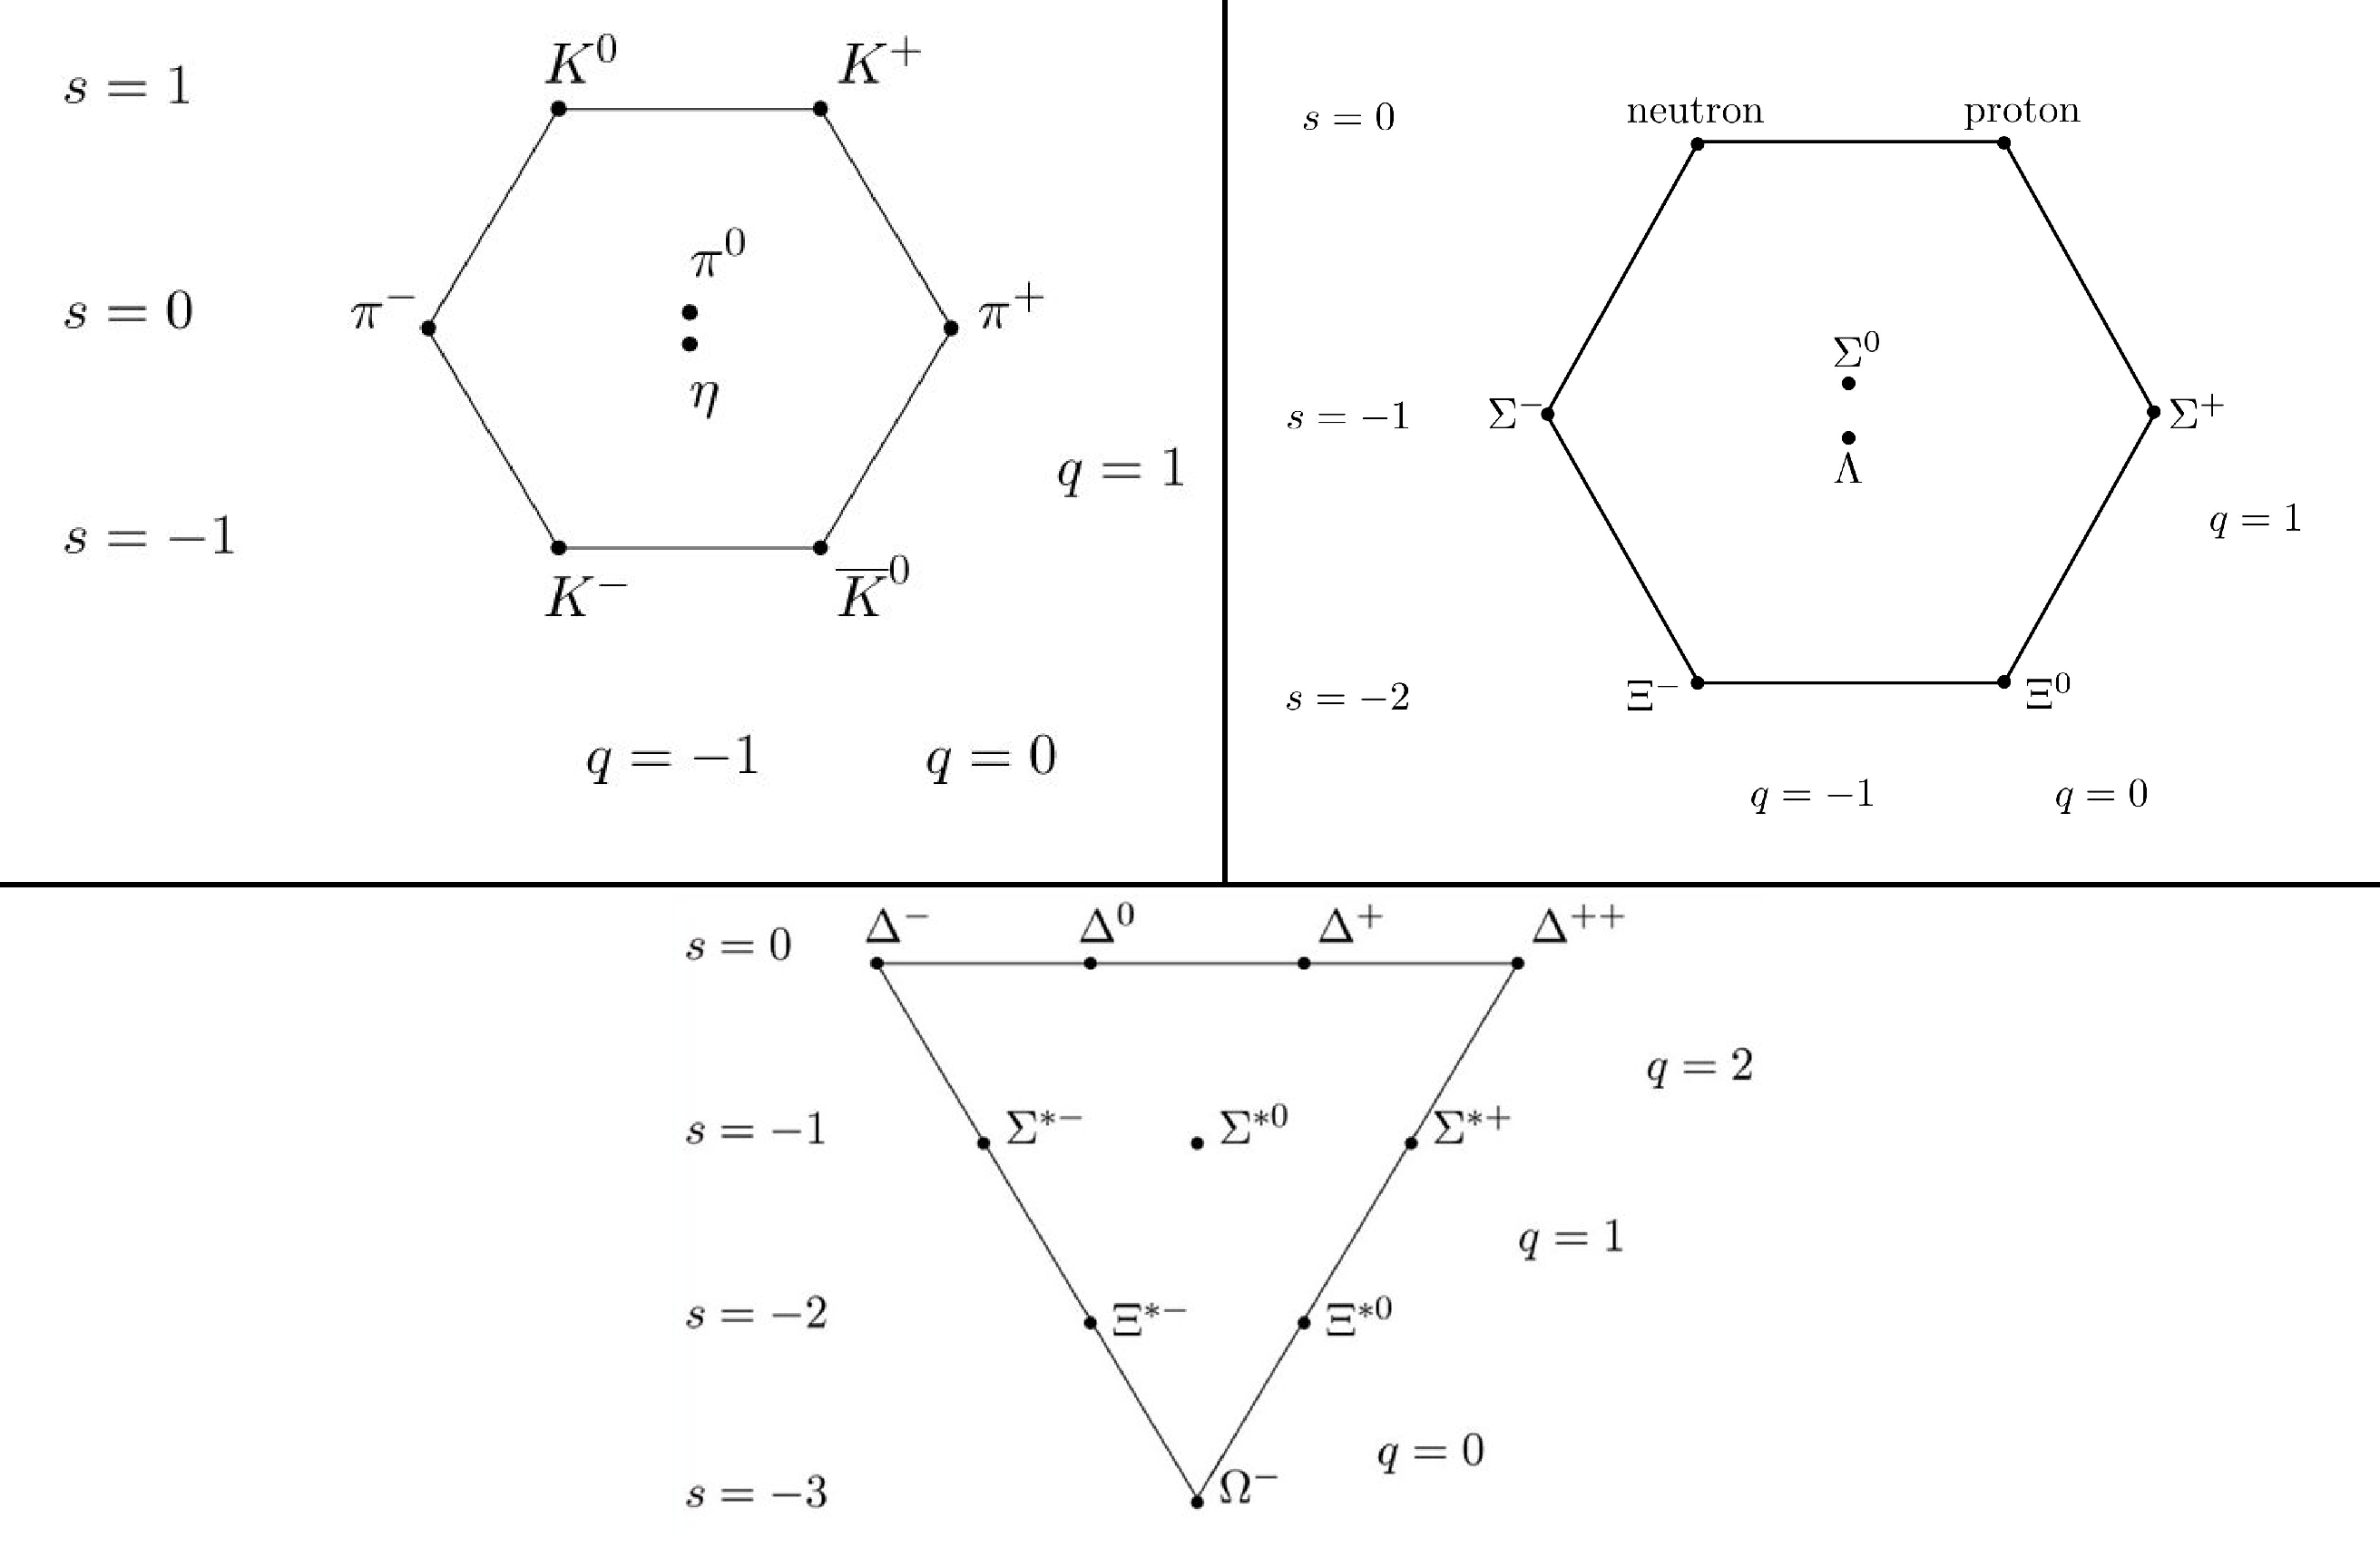
\includegraphics[width=5in]{figures/background/mesons_baryons.pdf}
	\caption{The octets and decuplet of Gell-Mann's ``Eightfold Way''. Top left: the eight particles of the meson octet; top right: the spin-$\frac{1}{2}$ baryon octet; bottom: the spin-$\frac{3}{2}$ baryon decuplet.}
	\label{fig:mesons-baryons}
\end{figure}

Near the end of the 1960's, SLAC began the first set of experiments to use an electron beam to investigate the nucleon in what is now known as Deep Inelastic Scattering (DIS). What they discovered was that the functions used to describe nuclear structure were largely independent of momentum transfer ($Q^2$) above a certain threshold. This so-called ``scaling'' behavior lent credence to the theory that nucleons were composed of point-like particles. This discovery coupled with the proliferation of new particles (the ``particle zoo'') led Murray Gell-Mann and Yuval Ne'eman to construct a framework that would make some sense of it all. Gell-Mann had organized the host of mesons and baryons discovered into a geometric order named the ``Eightfold Way''\footnote{Gell-Mann here makes a rather poetic allusion to the Buddhist ``Noble Eightfold Path''} as depicted in Figure~\ref{fig:mesons-baryons}. The underlying explanation for all of this, as described independently by Gell-Man and Ne'eman, was to characterize these many particles as the several combinations of three \emph{flavors} of constituent particles, named \emph{quarks}~\cite{joyce1999finnegans}. The flavors, \emph{u}, \emph{d}, and \emph{s} were named \emph{up}, \emph{down}, and \emph{strange}. Here, mesons were predicted to be composite particles of integer spin containing two quarks and baryons be half-integer spin particles composed of three quarks. This model led Gell-Mann to predict the existence of the $\Omega^-$ particle, along with its \emph{strangeness}, charge, and mass. The discovery of this particle~\cite{1964PhRvL:12204B} earned Gell-Mann the 1969 Nobel Prize for his work on the quark model.

Though this model was a breakthrough in the understanding of fundamental particles, it did not comprehensively describe all experimental data. For example, when accounting for the total momentum of a nucleon, it was found that only $\sim50\%$ of the momentum was being carried by the quarks. It was not until the theory of quantum chromodynamics (QCD) came along that this and several other mysteries could be explained. QCD described the mechanism of a 3-fold \emph{color} charge and the gauge bosons, gluons, that intermediate the strong force between quarks (and other gluons). In the particular case of the missing momentum, this was found to reside in the intermediating gluons~\cite{PhysRevLett.43.830}, which carry only color charge, to which the electroweak probes used were insensitive.

Many nuclear probes and methods have been used to characterize the distributions and characteristics of nuclear partons, including the aforementioned DIS process. As I will describe later in this section, much has been learned about parton probability distribution functions with this and other processes, but it is the process of hadron-hadron di-lepton production that is of primary focus in this paper, which allows for an alternative approach to investigate the structure and characteristics of the quarks inside of a nucleon, and perhaps shed some light on some ongoing mysteries in nuclear physics.

\section{Di-lepton production in nucleon-nucleon collisions}

Studying the production of pairs of leptons resulting from hadron-hadron collisions has proven to be a powerful tool in probing nucleon structure and parton distribution functions (PDFs). Figure \ref{fig:DY-spectrum} shows the mass spectrum of the muon mode of di-lepton production in proton-nucleus collisions measured at the E-866/NuSea experiment at Fermilab~\cite{PhysRevLett.80.3715}. The resonances of the $J/\Psi$, $\Psi^\prime$, $\Upsilon$, $\Upsilon^\prime$, and $\Upsilon^{\prime\prime}$ can be seen atop a smooth, continuous distribution which decreases with mass. The process responsible for this distribution of $\mu^+\mu^-$ pairs is the Drell-Yan process~\cite{PhysRevLett.25.316}, which is illustrated in the Feynman diagram in Fig.~\ref{fig:dy-diagram}. This process is characterized by a quark annihilating with an anti-quark to form a virtual time-like photon which then decays into a pair of leptons. The study of this process can lend some insight into nucleon structure due to the fact that the mass and momentum of the di-lepton pair directly reflects the momentum distributions of the interacting quarks and anti-quarks. The most comprehensive and precise knowledge and models of these momentum distributions come primarily from deep-inelastic lepton scattering (DIS) and the Drell-Yan (DY) process.

\begin{figure}
	\centering
	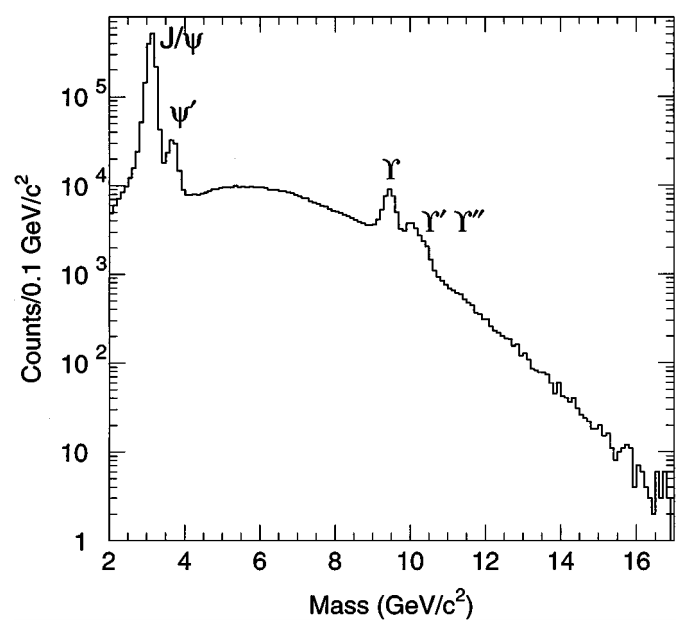
\includegraphics[width=3in]{figures/background/DY-spectrum-e866.png}
	\caption{Dimuon mass spectrum from E-866 $p+h$ collisions at \unit[800]{GeV/c}~\cite{PhysRevLett.80.3715}.}
	\label{fig:DY-spectrum}
\end{figure}

One particular focus of study for the Drell-Yan process is its nucleon number-dependent (A-dependent) behavior of its cross sections. This is of particular interest due to a phenomenon known as the EMC effect, in which the European Muon Collaboration (EMC) discovered in 1983 that parton distribution functions become modified when in the presence of the nuclear medium. This A-dependent behavior was not expected for hard scattering processes as the modest (maximum $\unit[8.8]{MeV}$) binding energy of a nucleus on a nucleon was not thought to have a significant effect on quark momentum distributions within a nucleon (\unit[938]{$Mev/c^2$}). Many experiments since have confirmed, extended, and precisely characterized the A-dependent behavior observed. Among the many hard scattering probes for investigating this phenomenon, the Drell-Yan process is uniquely capable of isolating the effect on the anti-quark distributions to a high degree of accuracy. The study of the effects of the nuclear medium on nucleon anti-quark distributions is the secondary research goal of the SeaQuest experiment and is the main focus of this thesis.

\subsection{The Drell-Yan Process}

\begin{figure}[h]
	\centering
	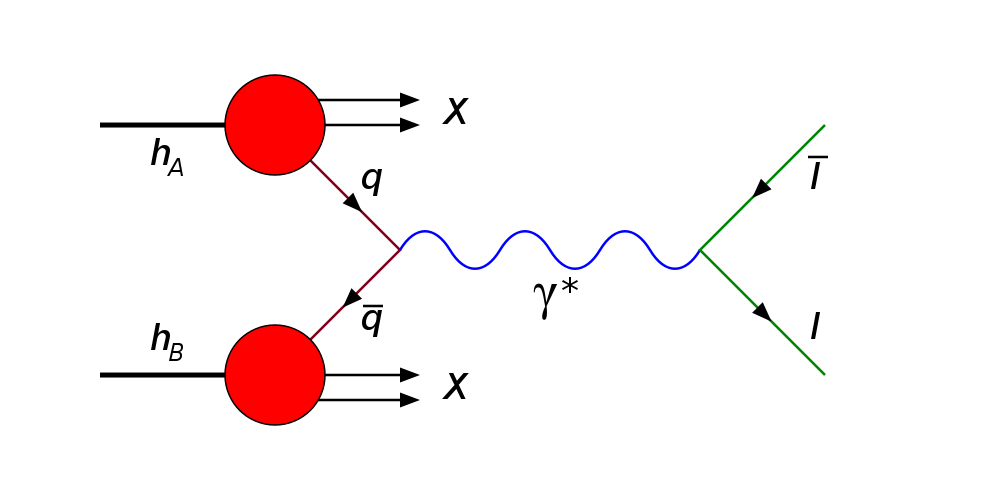
\includegraphics[width=4.5in]{figures/background/Drell-Yan.png}
	\caption{The Drell-Yan process, an $s$ channel interaction consisting of the annihilation of a quark with an anti-quark.}
	\label{fig:dy-diagram}
\end{figure}

The study of continuum di-lepton production in hadron collisions,
\begin{equation}
h_A +  h_B \rightarrow l^+ l^- + X
\label{eq:hh2ll}
\end{equation} 
can be used to study hadronic structure in a way that is complementary to the study of deep-inelastic scattering,
\begin{equation}
l + h \rightarrow l^\prime + X.
\label{eq:lh2lx}
\end{equation}
In 1970, S. Drell and T.M. Yan were the first to suggest that, at high $Q^2 (=M^2_{l^+ l^-}) \geq 16GeV^2$, the quarks inside the hadrons $h_A$ and $h_B$ can be considered free fermions in the instantaneous moment that they interact. The Drell-Yan model addresses the dominant subprocess here,
\begin{equation}
q_A + \bar{q}_B \rightarrow \gamma^* \rightarrow l^+ l^-
\label{eq:dy-process}
\end{equation} 
as an electromagnetic annihilation process. In this high-$Q^2$ kinematic space, the final state of the hadrons that contain these quarks becomes irrelevant. By the energy-time uncertainty principle~\cite{aHeisenberg:1927zz} of $\Delta E \Delta t \sim \hbar$, the timescales under consideration are $<10^{-25}s$, and the corresponding distances are $<10^{-17}m$, where the size of a nucleon is $\sim 10^{-15}m$~\cite{povh2002particles}. At these short space-time scales, electromagnetic annihilation dominates this quark-quark interaction.

This is further reinforced by the widely accepted non-Abelian gauge field theory of Quantum Chromodynamics (QCD) which describes the interactions between quarks and gluons. QCD provides a theoretical justification for treating Drell-Yan processes as events isolated from the rest of the hadron states, and it does so through the concept of the running of the coupling constant, or \emph{asymptotic freedom}~\cite{Bethke:2006ac}. This characteristic feature of QCD is described by the decrease of the strength of the strong force coupling constant as the space-time scale of the interaction approaches zero (i.e. as $Q^2 \rightarrow \infty$). The strong coupling constant can be expressed as a function of $Q^2$:
\begin{equation}
\alpha_s(Q^2) = \frac{1}{\beta_0 \ln (Q^2/\Lambda^2)}
\end{equation}
where
\begin{equation}
\beta_0 = \frac{12\pi}{33-n_f}
\end{equation}
Here, $\Lambda$ is the QCD scale parameter that depends on the number of quark flavors, $n_f$, and the renormalization scheme, measured to be around $\sim$ \unit[217]{MeV}. Experimental measurements of the running of the coupling constant as measured by many different processes can be seen in Figure~\ref{fig:asymptotic-freedom}.
\begin{figure}
	\centering
	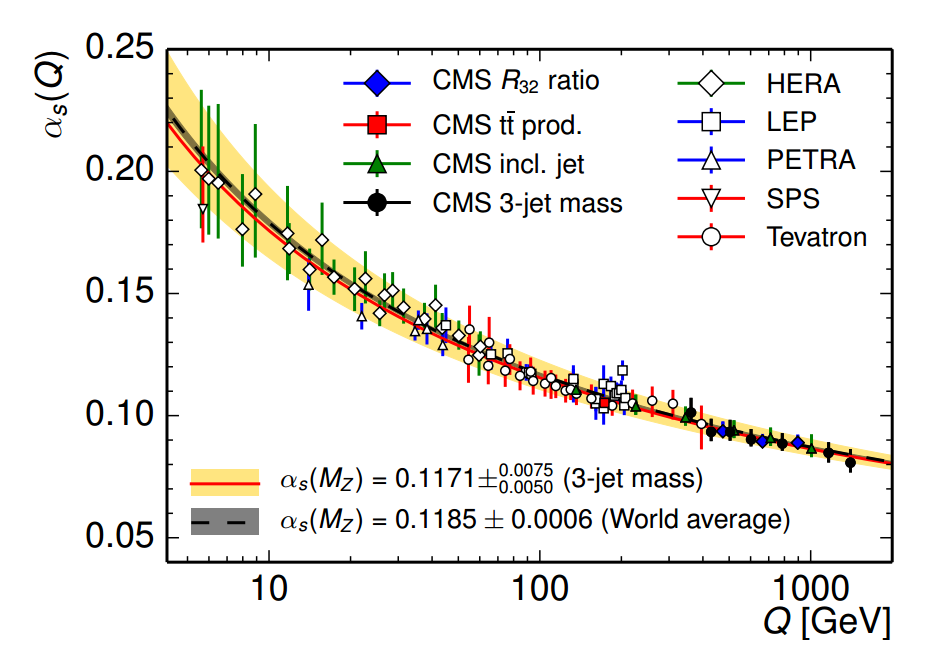
\includegraphics[height=3in]{figures/background/running-strong-coupling.png}
	\caption{A compilation of measurements of the running of the strong coupling constant, $\alpha_s(Q^2)$~\cite{CMS:2014mna}.}
	\label{fig:asymptotic-freedom}
\end{figure}

It is useful to have some intuition as to the reason for these ``running'' of the coupling constants. The phenomenon responsible are termed ``screening'' and ``anti-screening'' (or ``camouflaging'')~\cite{Quigg:1985ai}. This straightforward in the case of the electromagnetic force which can be seen depicted in the left pane of Figure~\ref{fig:screening-camo}. Whether it is in some kind of dielectric medium or in an isolated vacuum (where quantum fluctuations lead to virtual $e^+e^-$ pairs), the charges surrounding an individual charged particle are oriented in such a way as to decrease the overall observed charge. In the realm of QED, the higher energies you use to probe a particle, the closer you actually get to seeing the ``actual'' charge of the particle, and as such, the EM coupling constant increases at higher energies.

The same is seen in the case of QCD with its non-binary charge scheme. It's more difficult to conceptualize, but the same screening effect exists in the case of a particle with color charge. The middle pane of Fig.~\ref{fig:screening-camo} is a depiction of screening analogous to the familiar EM screening. The difference between QCD and QED with the behavior of the coupling constants is attributable to the fact that the force-carrying boson of QCD, the gluon, carries with it its own color charge. In the QED picture, the charge at the center is continuously emitting and absorbing photons as it interacts with the surrounding charges, but its charge does not change. With the color-charged particle, gluons are also being continuously emitted and absorbed, but an effect of that is a change in color charge. The result ends up being the phenomenon of camouflaging where the closer you are to a color-charged particle, the less that you can ``see'' the \emph{net} charge, and the actual charge of the particle is obfuscated. The net charge of the particle, statistically, becomes neutral, causing the strong force to become increasingly feeble at smaller scales (compared to the strength of QED interactions). This effect competes with and surpasses the color screening that occurs and is the root cause of the asymptotic freedom in QCD. On the flip side, the farther you get from the color charge, the more you are exposed to the full true net charge, and the stronger the coupling becomes. This increase in the coupling is the QCD confinement that is observed. An example if in the right pane of Fig.~\ref{fig:screening-camo} where the quark emits many gluons, thus changing its color from Blue to Green, but when summing over all colors emitted and absorbed, the net color is still Blue.

\begin{figure}
	\centering
	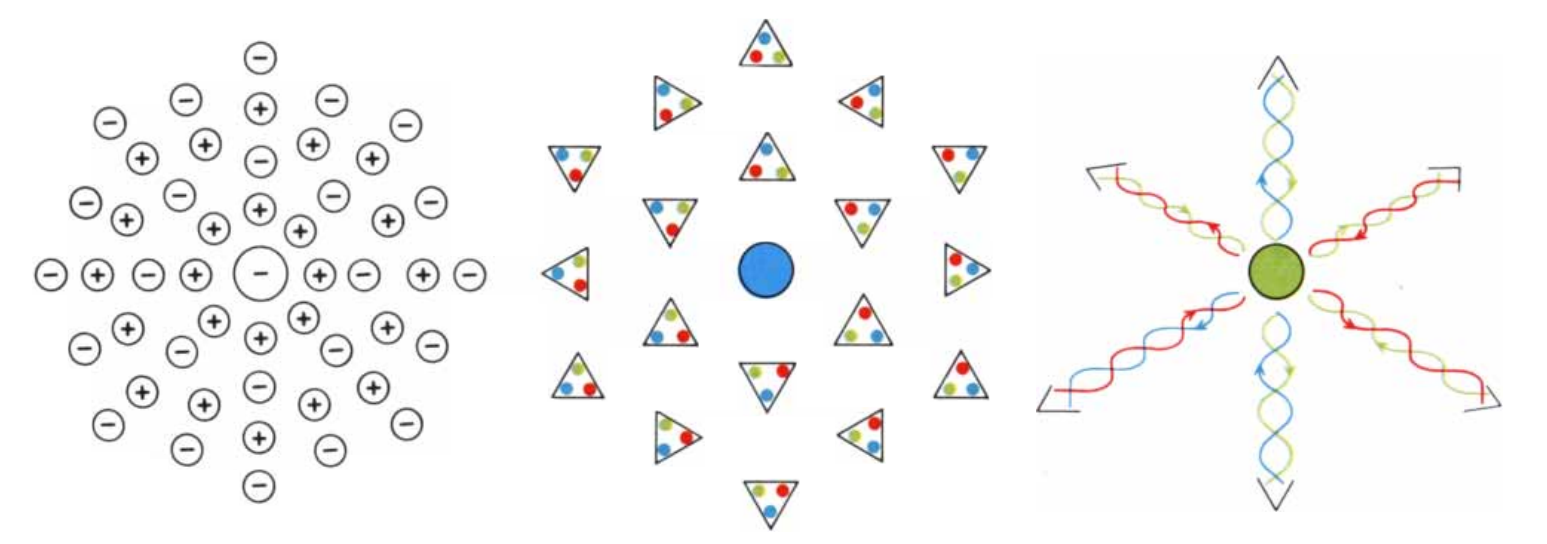
\includegraphics[width=\textwidth]{figures/background/screening-camo.png}
	\caption{(Left) classic electromagnetic screening of a free charge in a dielectric or even a vacuum. (Center) The analogous screening in the three-charge QCD regime. (Right) The color camouflaging due to the constant absorption/emission of colored gluons~\cite{Quigg:1985ai}.}
	\label{fig:screening-camo}
\end{figure}

\subsection{Drell-Yan Kinematics}

In the center-of-mass frame, the Drell-Yan process can be broken down into three stages with three sets of kinematics (refer to Fig.~\ref{fig:dy-diagram}). Beginning with the quarks, \emph{x} is defined as the fraction of the hadron's momentum carried by the interacting quark or antiquark. Conventionally in fixed-target experiments, subscripts are assigned as $x_1$ and $x_2$, which refer to the quark/antiquark from the beam and the antiquark/quark from the target, respectively. This \emph{x} is called the Bjorken \emph{x}, and is well-known in DIS processes to have a value of
\begin{equation}
x = -q^2/2 p \cdot q
\end{equation} where \emph{p} and \emph{q} are the 4-momenta of the hadron and the photon. In DY, the same momentum fraction $x$ is used to describe part of the fundamental basis of the interaction. In this case, $q$ is the 4-momentum of the virtual photon and $p$ is the 4-momentum of the hadron that contains the quark in question.

The next stage of the process is the virtual photon. This photon' properties are effectively equivalent to the `dimuon' or `dilepton', which are the terms more commonly used in referring to kinematics. The first of its relevant kinematics is its mass $M_{\gamma^*}$, which represents its energy and virtuality. The value $x_F$, or Feynman-x, is the fraction of the maximum possible longitudinal momentum carried by the virtual photon in the beam direction. The transverse momentum, $p_T$, and the azimuthal production angle, $\phi_{\gamma^*}$ are the remaining kinematics associated with the virtual photon.

The third stage regards the pair of leptons produced. In the frame of the virtual photon, there is a polar and azimuthal decay angle, $\theta_\mu$ and $\phi_\mu$, respectively, for each of the decay muons. It becomes impossible, however, to reconstruct these variables, as the individual transverse momenta of the quarks are unknown, and the thus the quark-antiquark annihilation axis is unknown. This is remedied by shifting the process into the Collins-Soper (CS) reference frame~\cite{PhysRevD.16.2219} which orients the reference axis to be parallel to the bisector of the angle between the interacting hadrons in the rest frame of the muon pair. A depiction of the Collins-Soper frame can be found in Fig.~\ref{fig:collins-soper}. In total, this brings a total of eight kinematic variables, summarized in Table~\ref{tab:var}.
\begin{figure}
	\centering
	\includegraphics[width=4.50in]{figures/background/three_plane.eps}
	\caption{A depiction of the Collins-Soper reference frame by Evan McClellan (UIUC). The CS variables are best understood by identifying the three defined planes and then referring to the specific angles between them.}
	\label{fig:collins-soper}
\end{figure}

Experimentally, six independent variables are measured, which form a basis by which all eight can be known. This is due to the fact that two pairs of variables, ($M_{\gamma^*}$, $x_F$) and ($x_1$, $x_2$) are correlated by the following, ignoring quark masses and considering $p_\perp << p_{\ell}$:
\begin{eqnarray}
x_F & \equiv & \frac{p_{\ell}}{\sqrt{s}/2} \approx x_1 - x_2 \label{eq:xf=x1-x2} \\
M_{\gamma^*}^2 & \equiv & E^2 - p_{\ell}^2  = s x_1 x_2 \label{eq:m=sx1x2} \\
E & = & \frac{1}{2}(x_1 + x_2) \sqrt{s} \\
p_{\ell} & = & \frac{1}{2}(x_1 - x_2)\sqrt{s}
\end{eqnarray}
In this frame, the longitudinal momenta of the quarks are $x_1 \sqrt{s}/2$ and $- x_2 \sqrt{s}/2$, with $\sqrt{s}$ being the center of mass energy of the hadronic collision. So, by measuring the 3-momenta of the $\mu^+$ and $\mu^-$, the quantities ($M_{\gamma^*}$, $x_F$, $p_T$, $\phi_{\gamma^*}$, $\theta_\mu$, $\phi_\mu$), which is sufficient to calculate the remaining ($x_1, x_2$) in our approximation.

\begin{table}[h]
	\centering
	\begin{tabular}{c|r}
		Variable&Description\\ \hline \hline
		$x_{1/2}$ & Momentum fraction of the beam/target quark\\
		$M_{\gamma^*}$ & Mass of the virtual photon (dimuon)\\
		$x_F$ & Fraction of the max. possible $p_{\ell}$ carried by virt. photon\\
		$p_T$ & Transverse momentum carried by the virt. photon\\
		$\theta_{\mu}, \phi_{\mu}$ & Polar and azimuthal decay angle\\ & of one of the muons, in the CS ref. frame\\ \hline
		$\alpha$ & The fine structure constant \\
		$K(x_1,x_2)$ & High-order QCD correction term \\
		$\sqrt{s}$ & Center of mass energy of the hadronic collision \\
		$\sqrt{\hat{s}}$ & Center of mass energy of the $q\bar{q}$ collision \\
		$Q^{2}$ & Four-momentum of the intermediate time-like photon, squared \\ 
		$q_i^{t/b}(x)$ & The quark number density in the nucleon of the target/beam \\ \hline \hline
	\end{tabular}
	\caption{Kinematic variables relevant to the Drell-Yan process .}
	\label{tab:var}
\end{table}

\subsection{Cross-Section}

As the participating quarks are asymptotically free within each hadron, there will be no correlations between the probability distributions of the annihilating particles, and the process is independent of the distributions. As a result, the cross section of the Drell-Yan process can be reduced to a function of the electromagnetic annihilation process and the quark probability distribution functions. With these components and some QCD considerations, we can construct it piece by piece.

The first step is to begin with the known hard scattering cross section of $\epsilon + \bar{\epsilon} \rightarrow l^+ l^-$, where $\epsilon$ is an arbitrary particle. This cross section\cite{Halzen:1984mc} is given by
\begin{equation}
\sigma(\epsilon\bar{\epsilon}\rightarrow l^+l^-) = \frac{4 \pi \alpha^2}{3M_{\gamma^*}^2} e_f^2
\label{eq:annihilation-cross}
\end{equation}
where $\alpha$ is the electromagnetic fine structure constant, $e_f$ is the charge of the particle, and $M_{\gamma^*}$ is the dilepton mass. With this, we add the QCD consideration that only $q\bar{q}$ of opposite color can annihilate with each other into a colorless virtual photon. Possible combinations are $R\bar{R}$, $B\bar{B}$, and $G\bar{G}$ out of $3\times 3$ possible cases. As such, an overall factor of $\frac{1}{3}$ is added to this cross section. Finally, factoring in the conservation of flavor (there can only be $u\bar{u}$, $d\bar{d}$, etc. combinations) and the quark structure of hadrons A and B,  we use the product ($q_f^A(x_1)\bar{q}_{f}^B(x_2)$) of the quark probability distributions for finding quarks of the same flavor-antiflavor combination in the two hadrons. It must also be considered that the quark or antiquark may be found in either hadron A or hadron B. The product of these three factors leads us to the Drell-Yan cross section\cite{Drell:1970wh}
\begin{eqnarray}
\frac{d^2\sigma}{dx_1dx_2}&=&\frac{1}{3}\frac{4\pi\alpha^2}{3M_{\gamma^*}^2}
\sum_{f}e_f^2[q_f^A(x_1)\bar{q}_f^B(x_2)+
\bar{q}_f^A(x_1)q_f^B(x_2)]\\
&=&\frac{4\pi\alpha^2}{9 s x_1 x_2}
\sum_{f}e_f^2[q_f^A(x_1)\bar{q}_f^B(x_2)+
\bar{q}_f^A(x_1)q_f^B(x_2)]
\label{eq:DY-cross}
\end{eqnarray}
where the sum is summing over flavors of quarks ($f\in\{u,d,s,...\}$). This can be evaluated in terms of the measurables $M_{\gamma^*}$ and $x_F$ via Equations~\ref{eq:xf=x1-x2}~and~\ref{eq:m=sx1x2}
\begin{equation}
M_{\gamma^*}^2 \frac{d^2\sigma}{dM_{\gamma^*}^2 dx_F} = 
\frac{1}{3}\frac{4\pi\alpha^2}{3M_{\gamma^*}^2}
\frac{x_1 x_2}{x_1 + x_2}
\sum_{f}e_f^2[q_f^A(x_1)\bar{q}_f^B(x_2)+
\bar{q}_f^A(x_1)q_f^B(x_2)]
\label{eq:dy-cs-observe}
\end{equation}
where $x_1$ and $x_2$ can be expressed as
\begin{equation}
x_1 = \frac{1}{2}\left[\sqrt{x_F^2 + 4\tau} + x_F\right],\ \  
x_2 = \frac{1}{2}\left[\sqrt{x_F^2 + 4\tau} - x_F\right],\ \ 
\tau = \frac{M_{\gamma^*}^2}{s}
\end{equation}
The cross section can also be represented by dimensionless variables in its scaling form,
\begin{equation}
s \frac{d^2\sigma}{d \sqrt{\tau} dy} = 
\frac{1}{3}\frac{4\pi\alpha^2}{3}
\sum_{f}e_f^2[q_f^A(x_1)\bar{q}_f^B(x_2)+
\bar{q}_f^A(x_1)q_f^B(x_2)]
\label{eq:dy-cs-dimensionless}
\end{equation}
where we introduce the rapidity term $y$ in describing $x_1$ and $x_2$,
\begin{equation}
y  = \frac{1}{2} \ln \frac{E+ p_\ell}{E-p_\ell} = \frac{1}{2} \ln \frac{x_1}{x_2},\ \ 
x_1  = \sqrt{\tau} e^{y},\ \  
x_2  = \sqrt{\tau} e^{-y}
\end{equation}
It should be noted that with collider experiments, it is conventional to refer to the hadrons A and B in terms of the beam and target hadrons, respectively, and as such, $x_1$ refers to the the quark in the beam hadron and $x_2$ refers to the quark in the target hadron.

In each of these equations~\ref{eq:DY-cross}, \ref{eq:dy-cs-observe}, and \ref{eq:dy-cs-dimensionless}, the cross sections can be factored into two parts: one subprocess cross section and one part that has only a dependence on the parton distribution functions. They are independent of each other because one of the staples of the quark parton model is that the PDFs ($q(x)$ and $\bar{q}(x)$) are independent of the process by which they are probed. This feature is commonly referred to as the ``universality'' of the PDFs.

\section{Nucleon Structure}

There are a few distributions, functions, terminologies, sum rules, and integrals that must be established and explained in order to speak the language of nucleon structure. Here, some of these are explained so that they may be used freely later. Also included are brief sections about how nucleon structure was tested by the Drell-Yan process, and how the QCD understanding of the nucleon was used to improve the understanding of the Drell-Yan process.

\subsection{PDFs, Structure Functions, and the Quark Parton Model}\label{sec:pdf}

In the context of hadron-hadron collisions, one can interpret the PDFs as follows: consider two hadrons A and B colliding; a parton of type \emph{a} ($a\in \{u, d, s, g, ...\}$) comes from A and carries with it a fraction of A's momentum ($x_A$).  The same goes for hadron B; a parton of type \emph{b} comes from B and carries momentum fraction $x_B$. Now, the probability of finding the discussed parton from A at momentum fraction $x_A$ is given by $q_{a/A}(x_A)$. Likewise, the probability of finding the discussed parton from B at $x_B$ is $q_{b/B}(x_B)$.

In general, experimental data measuring $F_2$ is used in conjunction with some general constraints in order to arrive at the calculated PDFs. One constraint is to consider the known number of valence quarks in a nucleon. Since the function $q_f(x)$ can be interpreted to be the number density of quark flavor $f$ as a function of momentum fraction $x$, the value $q_f(x)dx$ represents the number of quarks with flavor $f$ with fractional momentum in the range of $[x,x+dx]$. Therefore, the known number of valence quarks of flavor $f$ ($N_f$) provides the following condition.
\begin{equation}
\int_0^1 dx [q_f(x) - \bar{q}_f(x)] = N_{f}
\label{eq:vsr}
\end{equation}
Another condition considers the value $x q(x) dx$, which is the total momentum fraction of the hadron of the number of quarks $q(x)dx$. This provides a logical constraint is the summation of the momentum fractions of all partons must add up to the full nucleon momentum:
\begin{equation}
\sum_{q,\bar{q},g} \int_0^1 dx [x q(x)] = 1
\end{equation}
It should also be noted that the quark PDFs can be split with respect to their spin alignment ($+$) or anti-alignment ($-$) with the nucleon's spin
\begin{equation}
q(x) = q^+(x) + q^-(x)
\end{equation}
and the polarized (or helicity) PDF can be defined as
\begin{equation}
\Delta q(x) = q^+(x) - q^-(x)
\end{equation}
though, due to the fact that SeaQuest uses neither a polarized $\Delta q(x)$. There are two standing proposals, however, to extend the SeaQuest spectrometer for an additional period of data taking, augmenting it with a polarized proton beam (FNAL E-1027) and/or a polarized target (FNAL E-1039). The polarized beam proposal adds two beam-polarizing apparatuses named \emph{Siberian Snakes} to provide sufficiently polarized protons. The polarized target modification calls for the construction and installation of a new cryogenic liquid target system. Both proposals have been approved by the FNAL review committee and are likely to be acted upon near the end of the SeaQuest contract.

The structure functions $F_1, F_2,$ and $g_1$ of the nucleon are interpreted in the QPM as the charge-weighted sums over the quark flavors of the corresponding PDFs:
\begin{eqnarray}
F_1(x) = \frac{1}{2} \sum\limits_f e_f^2 q_f(x) \label{eq:f1} \\
F_2(x) = \sum\limits_f e_f^2 x q_f(x) \label{eq:callan-gross} \label{eq:f2} \\
g_1(x) = \frac{1}{2} \sum\limits_f e_f^2 \Delta q_f(x) \label{eq:g1}
\end{eqnarray}
where here $f$ represents all flavors of of quarks and anti-quarks. We see above the relation between $F_1(x)$ and $F_2(x)$ known as the Callan-Gross relation ($F_2 = 2xF_1$). This relation relies on the partons having spin-$\frac{1}{2}$ and no transverse momentum in the infinite momentum frame. The full expression is
\begin{equation}
F_2 = 2xF_1 \frac{1 + R}{1 + 2 M_N x/\nu}
\end{equation}
where $M_N$ is the nucleon mass and $R=\sigma_L/\sigma_T$ is the ratio of cross sections for absorbing a longitudinal to that for a transverse photon. Experimentally, R is small\cite{PhysRevLett.61.1061} ($\lesssim0.1$) for $x\gtrsim0.1$ and for $Q^2\gtrsim$\unit[5]{GeV$^2$}. Also, when assuming the infinite momentum frame, $\nu$, the energy transferred by the photon is assumed to trend towards infinity. As a result, this relation reduces to the commonly-used Callan-Gross relation.

Due to the complex nature of lattice QCD\footnote{An approach to solving quantum chromodynamics situations by simulating quarks and gluons on a set of lattice points in spacetime and modeling their well-defined interactions.} simulations, the parton distributions $q_f(x)$ and $\bar{q}_f(x)$ within the nucleus are determined empirically, with only a few rules based on theory. The primary probe used to measure them has been deep inelastic scattering (DIS), examining the inclusive jet production in order to get a clearer picture of nucleon structure. Data from many different experiments are combined  to extract the unpolarized PDFs. The earlier parametrizations of the PDFs first relied on fits to the measured structure functions solely from DIS experiments which are primarily sensitive to the light quark distributions and are unable to distinguish between quarks and antiquarks of the same flavor. More modern parametrizations use many different processes to extract supplementary and complementary information that can be incorporated. Lepton-charge asymmetry observed in $W^\pm$ production provides additional light quark distribution information. Jet production and photon measurements are also used to set constraints on gluon distributions. It should be noted that Drell-Yan dilepton production from such experiments as E605 and E866 that have contributed constraints on the light anti-quark distributions from the nucleon sea.

Current experimental determinations of these PDFs compiled by CTEQ (Coordinated Theoretical-Experimental Project on QCD) and TEA and are illustrated in Figures~\ref{fig:pdf-q2}~and~\ref{fig:pdf-q100}. The CTEQ-TEA calculated these PDFs from data on inclusive, high-momentum transfer processes, for which perturbative QCD is expected to be reliable. In the case of deep inelastic lepton scattering, only data with $Q > 2$ GeV is used. Data in this region are expected to be relatively free of non-perturbative effects, such as higher twists or nuclear corrections. Thus, there is no need to introduce phenomenological models for nonperturbative corrections beyond the leading-twist perturbative contributions\cite{Dulat:2015mca}.

\begin{figure}
	\centering
	\subfloat[][PDFs $x f_q(x, Q)$ for Q=2 GeV.]{%
		\label{fig:pdf-q2}%
		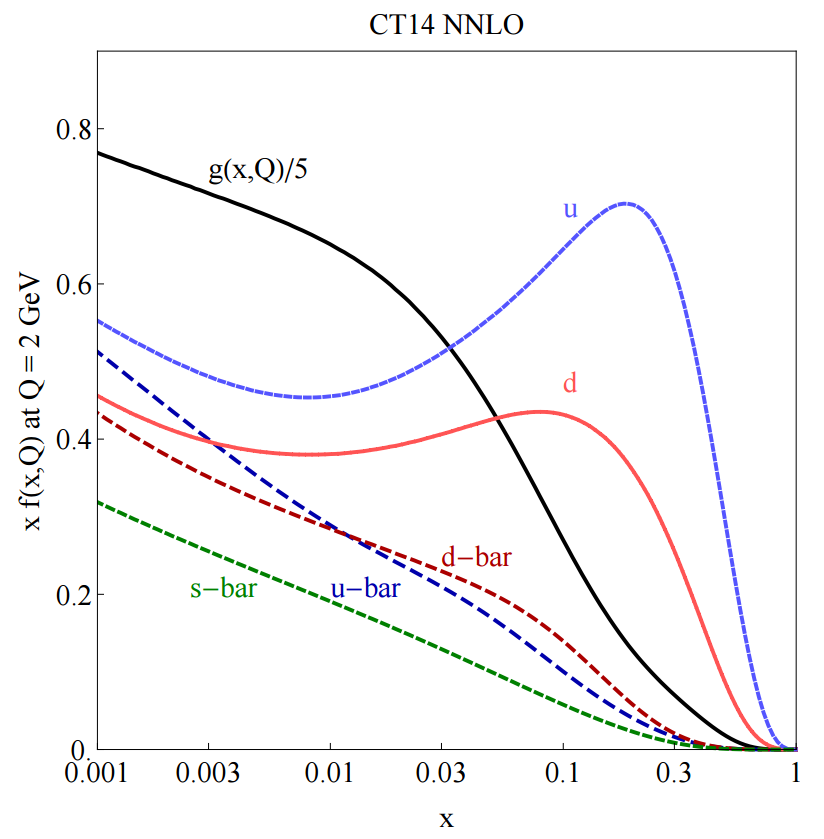
\includegraphics[width=0.45\linewidth]{figures/background/parton-dist-q2.png}}
	\hspace{8pt}%
	\subfloat[][PDFs of $x f_q(x, Q)$ for Q=100 GeV.]{%
		\label{fig:pdf-q100}%
		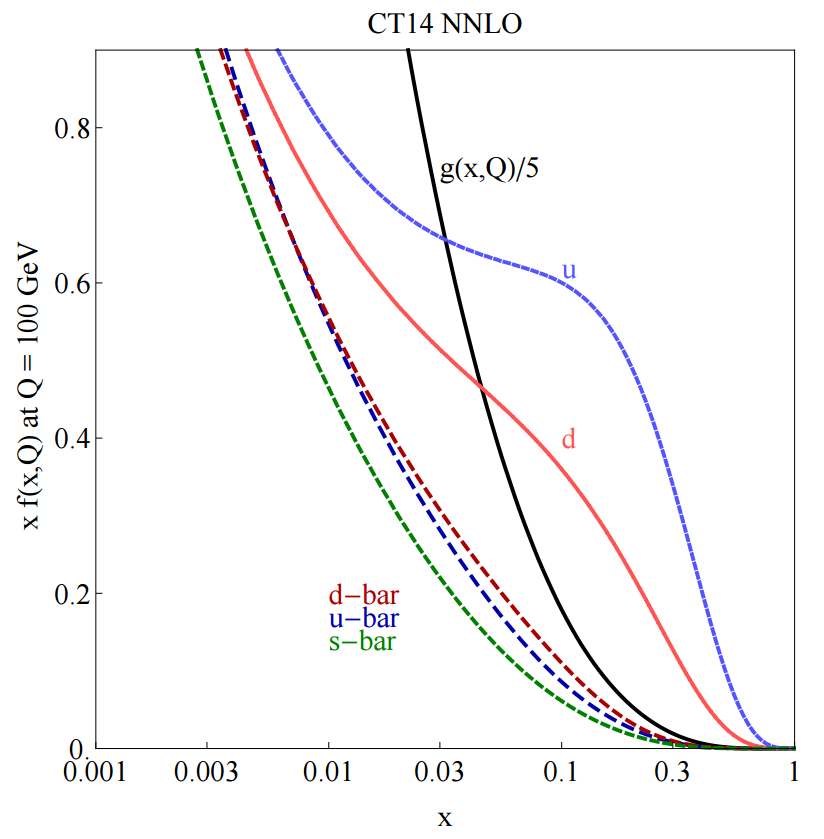
\includegraphics[width=0.45\linewidth]{figures/background/parton-dist-q100.png}}
	\caption{Parton distribution functions for quarks and gluons and their \emph{x} and \emph{Q} dependence as calculated to NNLO by the CTEQ-TEA (CT) global analysis group\cite{Dulat:2015mca}.}
	\label{fig:pdf-q2-q100}
\end{figure}

Looking to Figure~\ref{fig:pdf-q2-q100} we see that at $x>0.1$, $u$ and $d$ quarks dominate $\bar{u}$ and $\bar{d}$ quarks. The SeaQuest spectrometer (described in detail in the next chapter) is a ``forward spectrometer'', which means that, for PDF-relevant purposes, the high-$x_F$ ($x_F>0$) kinematic phase space is explored, which translates to high $x_1$ and low $x_2$. With this consideration, the Drell-Yan process measured at SeaQuest is probabilistically dominated by a quark from the beam annihilating with an anti-quark from the target. Further, all anti-quarks that exist in the target nucleons must come from what are called the \emph{sea quarks}, or the virtual $q\bar{q}$ pairs 
that arise from gluons splitting. 

Other interesting observations and measurements that have gone into these distributions are the observations of momentum contributions from all quarks and antiquarks and the momentum fraction from just antiquarks. The momentum sum
\begin{equation}
x_{tot} = \int_0^1 dx [F_2(x)] \simeq \int_0^1 dx [x(q(x) + \bar{q}(x))] \label{eq:mom-sum}
\end{equation}
showed that $x_{tot}$ for quarks is $0.512 \pm 0.018$~\cite{griffiths2008introduction}. The rest was found to be attributed to the gluons, though they could not be detected directly by an electron beam in DIS since they carry no electric charge. The momentum fraction from just anti-quarks comes from clever use of another structure function, $F_3$.
\begin{eqnarray}
F_3^{\nu N}(x) & = & q(x) - \bar{q}(x) - 2s(x) + 2c(x) \\
F_3^{\bar{\nu} N}(x) & = & q(x) - \bar{q}(x) + 2s(x) - 2c(x) \\
F_3(x) & = & \frac{1}{2} [F_3^{\nu N}(x) + F_3^{\bar{\nu} N}(x)] = q(x) - \bar{q}(x) = u_v(x) + d_v(x)
\end{eqnarray}
Here, the $v$ subscript denotes valence quark distributions, $q/\bar{q}(x)$ are
\begin{eqnarray}
q(x) & = & u(x) + d(x) + s(x) + c(x) \\
\bar{q}(x) & = & \bar{u}(x) + \bar{d}(x) + \bar{s}(x) + \bar{c}(x)
\end{eqnarray}
and the individual $F_3^{\nu/\bar{\nu}N}$ structure functions are measured from $\nu N$ and $\bar{\nu} N$ scattering and then combined With $F_3$, there is the Gross-Llewellyn Smith (GSL) sum rule\cite{Gross:1969jf}
\begin{equation}
\int_0^1 F_3(x) = 3
\end{equation}
which is to say that there are three valence quarks. The new information gained here with $F_3$ though is the measurement of $\int dx [xF_3(x)] = 0.341 \pm 0.036$, which gives the momentum fraction carried by the valence quarks. Put this together with the results of Eq.~\ref{eq:mom-sum} and one can derive the conclusion that the anti-quarks in the nucleon possess between 13\% and 17\% of the nucleon's momentum\cite{Fisk:1982pn}.

The last interesting sum rule to discuss is the Gottfried sum rule which is focused on flavor asymmetries between the proton and its isospin partner, the neutron.
\begin{eqnarray}
S_G & = & \int_0^1 dx \left[\frac{F_2^p - F_2^n}{x}\right] \\
& = & \int_0^1 dx \left[ \sum\limits_f e_f^2 [q_f^p(x) + \bar{q}_f^p(x) - q_f^n(x) - \bar{q}_f^n(x)] \right]
\end{eqnarray}
We assume charge symmetry insofar as $u^p(x) = d^n(x)$ and $\bar{u}^n (x) = \bar{d}^p(x)$, yielding
\begin{equation}
S_G = \int_0^1 dx \left[ \frac{1}{3} (u(x) + \bar{u}(x) - d(x) - \bar{d}(x)) \right]
\end{equation}
where these PDFs refer to the distributions in the proton. By some reorganization and grouping, this can be re-expressed in a more familiar way.
\begin{equation}
S_G = \int_0^1 dx \left[\frac{1}{3} [u(x) - \bar{u}(x)] \right] - 
\int_0^1 dx \left[\frac{1}{3} [d(x) - \bar{d}(x)] \right] -
\int_0^1 dx \left[\frac{2}{3} [\bar{d}(x) - \bar{u}(x)] \right]
\end{equation}
The first two integrals here are the definitions of the valence quark sum rule mentioned in Eq.~\ref{eq:vsr}, and this is known to be 2 and 1 for the $u$ and $d$ valence quarks of the proton, respectively. As a result, we arrive at the common representation of the Gottfried Sum Rule (GSR)~\cite{Gottfried:1967kk}.
\begin{equation}
S_G = \frac{1}{3} - \int_0^1 dx \left[ \frac{2}{3} [\bar{d}(x) - \bar{u}(x)] \right]
\label{eq:gsr}
\end{equation}
If one were to assume that, within a proton, $\int dx [\bar{u}(x)] = \int dx[\bar{d}(x)]$, then this sum reduces to $\frac{1}{3}$. More on this sum and its measured violation in Section~\ref{sec:dbar-ubar}.

\subsection{Drell-Yan Tests of the QPM}

The Drell-Yan process can be described within the frameworks of QPM and QCD, so it provides a good testing ground for these models. Even further, the very clean leptonic DY signature offers a good vantage point by which to confirm the parton picture experimentally. The testing process began with establishing the validity of the quark parton model via Drell-Yan. Once this is done, the following step would be to study the deviation between measurements and what is expected. Here we step through some tests of the QPM that Drell-Yan was applied to in order to validate.

\subsubsection{Point-like quarks}

If the quarks in the QPM are point-like and without any substructure, then the DY cross section (expressed in Eq.~\ref{eq:dy-cs-dimensionless}) across $Q^2$ should exhibit scaling behavior, i.e. the parton distributions measured should be $Q^2$-invariant. The experiments E-288 and E-605 at Fermilab compared the cross section yields across four different beam energies corresponding to $\sqrt{s}$ values between 19.4 and \unit[38.8]{GeV}. For each setting, the cross section was binned in $x_1$ and $x_2$ and compared across different beam settings (this is the same as binning in $Q^2=M_{\gamma^*}=sx_1x_2$).

If the what was being seen was a quark, and the quark was point-like, then the cross section would be $Q^2$-independent. If there was substructure to the quark, then at higher $Q^2$, sub-quarks would strike or annihilate with other sub-quarks, and one would observe the cross section increasing with $Q^2$ as new interaction phase space becomes available. The measurements of the experiments exhibited no $Q^2$-dependence~\cite{PhysRevD.23.604, Brown:1989fj} and lent support to the notion that what was being struck was indeed a point-like particle with no sub-structure.

\subsubsection{Quark charge}

One of the predictions of QPM was that the up (down) quarks possessed $e_u=+2/3$ ($e_d=-1/3$) times the elementary charge. The use of $\pi^+$ and $\pi^-$ beams to induce Drell-Yan interactions was used in the Fermilab E-444 and the OMEGA experiments to measure the Drell-Yan cross section ratios of $\pi^+$ to $\pi^-$, which should approach a value of $\frac{e^2_d}{e^2_u}$. The results indicated a value of $\frac{1}{4}$~\cite{GrossoPilcher:1986nk, Hogan:1979tu}, which is consistent with at least the magnitudes of the charges of the quarks.

\subsubsection{Spin-1/2 quarks}

If the quarks that annihilate are in fact spin$-\frac{1}{2}$ particles, then the virtual photon that the quarks annihilate to must be predominantly transversely polarized. This, in turn, should define the angular distribution of the leptons that are produced. As such, a transversely polarized photon should result in a dilepton distribution that goes as $dN/d\theta = 1+\cos^2\theta$ in the rest frame~\cite{Kenyon:1982tg}.

Several experiments sought to test this prediction, but the values of the measurement where $\cos\theta \approx \pm 1$ had a lack of data, allowing for a sizable amount of variation. Regardless, the data collected by CIP, NA3, ABCS, CHFMNP, Omega, and Goliath all fit the angular distribution to the function $f(\theta)=1+\lambda\cos^2\theta$ and arrived at results for $\lambda$ consistent with $\lambda=1$, though each had relatively sizable uncertainties~\cite{Kenyon:1982tg}. This is in agreement with what the simple Drell-Yan model predicts.

\subsection{QCD-Improved Drell-Yan}

According to the quark-parton picture, the simple Drell-Yan model predicts a certain magnitude of the cross-section and a certain measurement of $p_T$. Deviations from these predictions indicated a need to accommodate for higher-order effects that arise due to QCD effects. 

It was determined over the course of many experiments that the shape of the cross section was predicted very well while the scale of the measurement was off by a non-negligible amount. The discrepancy was studied thoroughly in the form of an arbitrary correction constant, $K$, known as the $K$-factor:
\begin{equation}
\frac{d\sigma^{DY}}{dQ^2}\bigr|_{exp} = K\cdot \frac{d\sigma^{DY}}{dQ^2}\bigr|_{LO}
\end{equation}
where LO stands for leading order (NLO, NNLO stand for next-to- and next-to-next-to-leading order). Relatively wide ranges of values of $K$ were measured~\cite{GrossoPilcher:1986nk}, from 1.6 to 3.1, with the combined value converging to around 2.

The expected measurement of $p_T$ was also surprising, as the simple Drell-Yan predicted a simple, clean annihilation that carried no other $p_T$ than the intrinsic $p_T$ caused by nucleon confinement and Fermi motion, which should be on the order of \unit[400]{MeV} (this value depends on the proton dimensions only). It turned out that not only did the measurement of $p_T$ not match this constant value, but the Omega collaboration showed that the value had a dependence on the $\sqrt{s}$ in the form of 
\begin{equation}
\hat{p}_T^p = 0.45 + 0.025 \sqrt{s}\ \ \ ; \ \ \ \hat{p}^\pi_T = 0.54 + 0.029 \sqrt{s}
\end{equation} for proton-induced pion-induced DY, respectively~\cite{Kenyon:1982tg}.

\begin{wrapfigure}{L}{0pt}
	\centering
	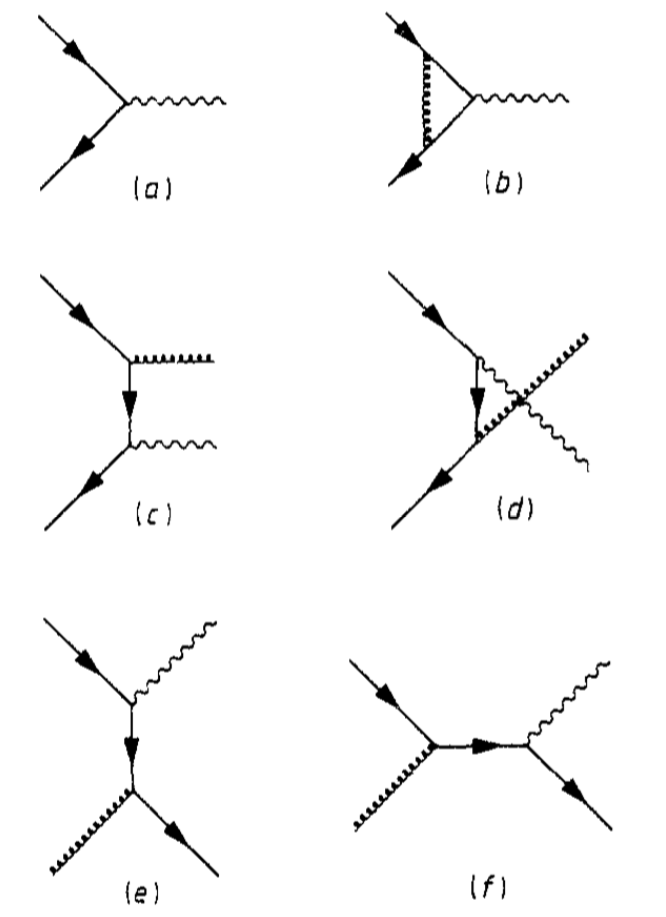
\includegraphics[width=0.45\textwidth]{figures/background/DY-NLO.png}
	\caption{Diagrams of (a) LO Drell-Yan, (b) vertex correction, (c-d) gluon emission, (e-f) ``Compton'' scattering~\cite{Kenyon:1982tg}.}
	\vspace{-20pt}
	\label{fig:DY-NLO}
\end{wrapfigure}
These discrepancies can be understood when one considers gluon interactions that happen on very short time scales. When a quark participates in a DY interaction, it may emit a gluon before encountering the other quark. The effects of time dilation in the moving nucleon essentially result in this (\emph{soft}) gluon happening ``long before'' the hard interaction occurs. This will not alter the factorized structure of the Drell-Yan cross section. It is, however, the case that gluon emission and absorption can occur at timescales on the order $\Delta t \sim 1/Q$ before the actual annihilation (i.e. \emph{hard} gluons). 

Several different hard gluon interactions that do affect the Drell-Yan cross section can be seen in Figure~\ref{fig:DY-NLO}.  In part (a), the LO DY vertex is shown, and the rest are the correction graphs that must be accounted for. Diagram (b) shows a vertex correction term, (c) and (d) show gluon emission in the final state, and (e) and (f) show QCD ``Compton'' scattering~\cite{Kenyon:1982tg}. Of these processes, diagrams (c-f) show a virtual photon recoiling off of an outgoing gluon, and these together easily account for the additional $p_T$ that is produced. 

The $K$ factor has been found to be generally of the form $K = \exp[(\alpha_s/2\pi)(4\pi^2/3)]$, and has been calculated in considerable detail~\cite{Matsuura:1988sm} to order $\bigoh(\alpha_s^2)$ and are considered to be under control. Most importantly, it was found at the E-866 experiment that the differential cross section ratios in the next-to-leading order are almost identical to those in the leading order nuclear dependence (at \unit[800]{GeV})~\cite{Duan:2004cw}. Further, similar results are given for the lower energy proton bombarding deuterium and tungsten at the Fermilab Main Injector (FMI, \unit[120]{GeV} proton beam)~\cite{Geesaman:906prop} which is used at SeaQuest. Therefore, QCD corrections for nuclear targets (compared to free nucleons) can be considered negligible. As such, when taking ratios of cross sections of different nuclear materials, the $K$-factors are considered to cancel each other out.

\section{Drell-Yan and Sea Quark Phenomenology}

Interestingly enough, the nucleon is not simply a particle composed of three quarks held together by intermediating gluons. Instead, due to the coupling strength of the strong force and the ability of gluons to couple to gluons, the proton is an impressively complex structure with evanescent virtual quark pairs (and even virtual mesons). Unfortunately, there is difficulty in isolating the specific features of this \emph{nucleon sea} using the tried and true DIS that had so thoroughly investigated nucleon structure. In this regard, the Drell-Yan process has proven to be crucial in the exploration of the nucleon sea, despite its small cross section. In this section, I discuss the discovery of sea quark asymmetry the meson cloud model (one of many) that attempts to describe it.

\subsection{$\bar{d}/\bar{u}$ Asymmetry}\label{sec:dbar-ubar}

Even though the quark sea flavor asymmetry is not the main focus of this paper, it is the flagship measurement of the SeaQuest experiment. As such, much of the work that will be explained in later chapters is common to the $\dbar/\ubar$ analysis, and so it is worth touching on its importance here.

The Gottfried Sum Rule (Eq.~\ref{eq:gsr}) can be seen as a measure of flavor symmetry (or asymmetry) in the nucleon. If flavor symmetry were to be upheld, then the sum would strictly be $S_G = \frac{1}{3}$. The New Muon Collaboration (NMC) at CERN sought to test this by measuring the cross section ratio for DIS of muons on hydrogen to muons on deuterium~\cite{Amaudruz:1991nw,Arneodo:1994sh}. This cross section ratio allowed for the measurement of $F_2^n/F_2^p$ over a Bjorken-$x$ range of $0.004 < x < 0.8$.  Incident muon energies of \unit[90]{Gev} and \unit[280]{GeV} were used to measure the $F_2$ ratio at $Q^2$ of \unit[4]{GeV$^2$}. The full results of the NMC experiment can be seen to be in clear disagreement with flavor symmetry in Figure~\ref{fig:nmc}. The extrapolated result of the NMC measurements over all $x$ yielded
\begin{equation}
S_G = \int_0^1 dx \left[ \frac{F_2^p - F_2^n}{x} \right] = 0.235 \pm 0.026.
\end{equation}

\begin{figure}
	\centering
	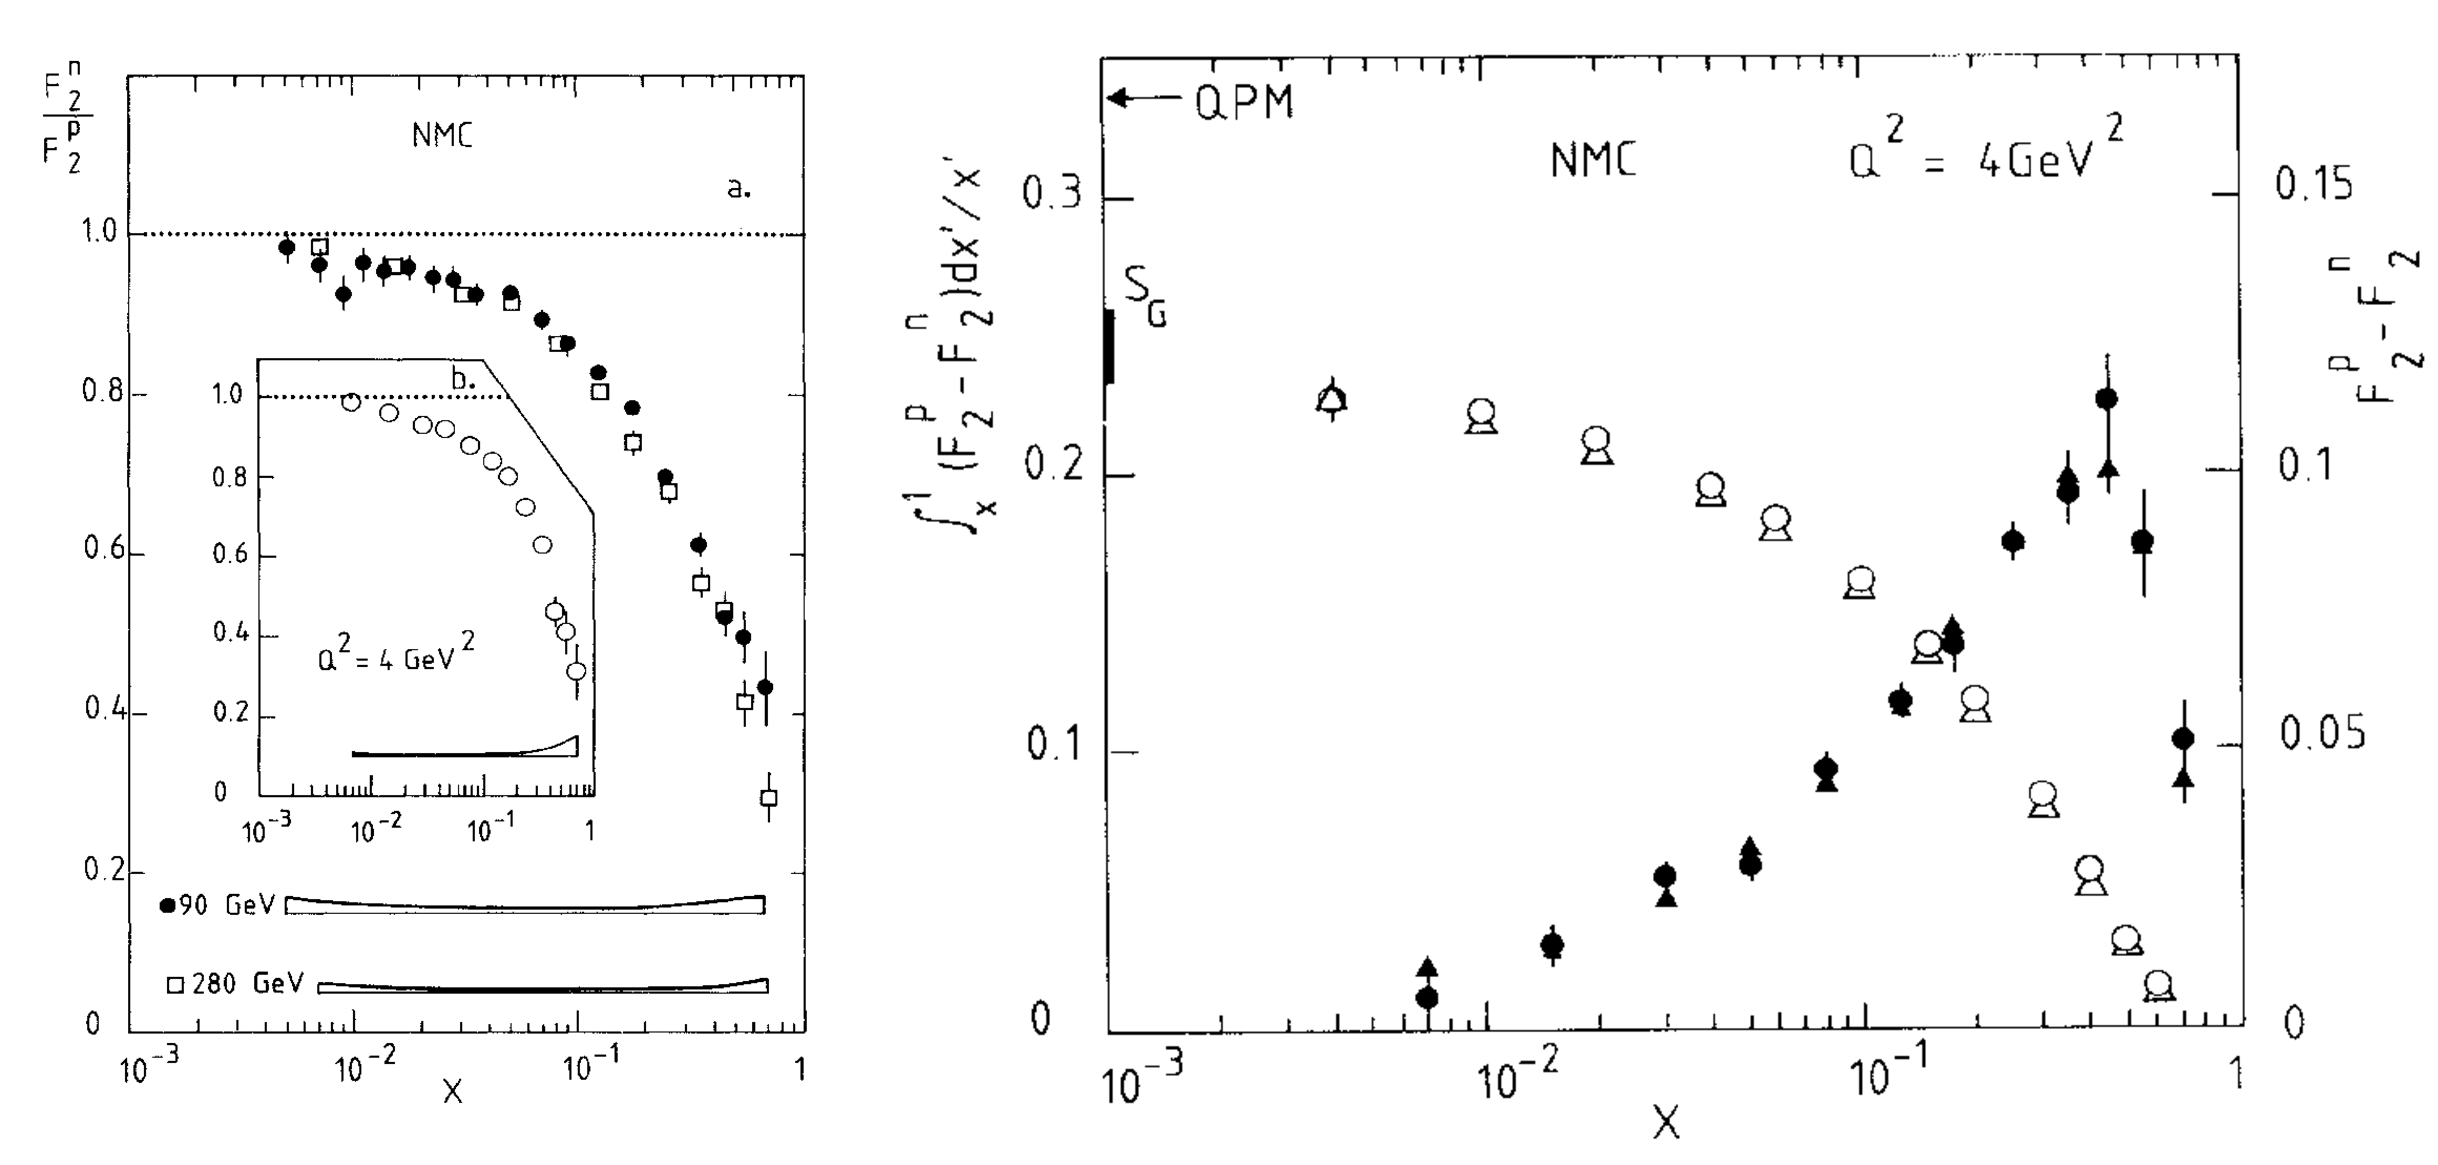
\includegraphics[width=\textwidth]{figures/background/NMC-All.pdf}
	\caption{The NMC experimental measurements of (left) $F_2^n/F_2^p$ and (right) the Gottfried Sum ($S_G$) with $\frac{1}{3}$ denoted by ``QPM''.}
	\label{fig:nmc}
\end{figure}

To reconcile this result with the QPM expectation, certain assumptions need to be reevaluated. The first assumption is that the extrapolation of the NMC result to low $x$ is correct. The second is that charge symmetry is valid. The final assumption is the flavor symmetry of the quark sea, or, $\int dx [\bar{d}(x)] = \int dx [\bar{u}(x)]$. The E-665 experiment at FNAL sought to extend the NMC low-$x$ coverage ($10^-6 < x < 0.3$) despite the difficulties of DIS in the extremely low-$x$ range. The results were consistent with NMC's extrapolation~\cite{Adams:1995sh}, and so the faulty assumption must lie elsewhere. Charge symmetry violation would lead to such a discrepancy, but to date, charge symmetry has been upheld in the relevant energy regime~\cite{Abegg:1998sg}. This leaves only $\int dx [\bar{d}(x)] = \int dx [\bar{u}(x)]$ being violated to account for the difference, and if it were to be the root cause, the contribution to the violation would be
\begin{equation}
\int_0^1 dx[\bar{d}(x) - \bar{u}(x)] = 0.148 \pm 0.039.
\end{equation}
As such, this conclusion was the first indicator pointing to the existence of more anti-down than anti-up quarks in the quark sea. This prompted further investigation of nucleon sea anti-quark asymmetry.

Following the NMC results, it was suggested~\cite{Ellis:1990ti} to exploit features of the Drell-Yan process as a direct probe of nucleon sea distributions. The most direct method of doing so is to measure the Drell-Yan cross-sections for both hydrogen and deuterium and take the ratio of the two. The proton-deuterium cross section can be seen as a convolution of cross sections of proton-proton and a proton-neutron
\begin{equation}
\sigma^{pd} \approx \sigma^{pp} + \sigma^{pn}
\end{equation}
ignoring any small nuclear effects or phenomenon that may exist in the deuteron. In this picture, the deuterium-to-hydrogen DY ratio yields can be used to determine $\dbar/\ubar$.

The NA51 experiment at CERN~\cite{Baldit:1994jk} used a \unit[450]{GeV/c} primary proton beam ($\sqrt{s}=$\unit[29]{GeV}) from CERN-SPS on deuterium and hydrogen targets to measure $\sim$6000 Drell-Yan dimuon events, cutting on $M_{\gamma^*}>$\unit[4.3]{GeV}. The reason for the mass cut is to investigate the Drell-Yan continuum as depicted in Figure~\ref{fig:DY-spectrum} and exclude any possible signal contamination from heavy quarkonia. The NA51 experiment looked to measure what it called the ``p$-$n cross section asymmetry'' of the Drell-Yan process:
\begin{eqnarray}
A_{DY} & = & \frac{\sigma_{pd}-\sigma_{pp}}{\sigma_{pd}+\sigma_{pp}} = 2\frac{\sigma_{pp}}{\sigma_{pd}} - 1 \\
A_{DY} & = &  -0.09 \pm 0.02 (\text{stat}) \pm 0.025 (\text{sys})
\end{eqnarray}
which was used to obtain a value for $\dbar/\ubar$. However, due to the NA51 spectrometer being designed to select rapidity about $y=0$ along with having low statistics, NA51 only provided a single value for this measurement centered at $x_F=0$ and $x=0.18$.
\begin{equation}
\frac{\dbar}{\ubar} \Bigr|_{\langle x \rangle = 0.18} = 1.96 \pm 0.15\text{(stat)} \pm 0.19\text{(sys)}
\end{equation}
This provided strong evidence in confirmation that there was indeed a $\dbar$ excess in the nucleon. Unfortunately, without more statistics, no $x$-dependent behavior of this asymmetry could be determined. This NA51 result coupled with that of NMC prompted several groups to perform global fits from DIS and DY data with the consideration that $\dbar\neq\ubar$, though no $x$-dependent constraints could be imposed on the $\dbar(x)/\ubar(x)$.

An improved experimental design of a ``forward'' muon spectrometer ($x_F>0$) was devised and implemented by the E-866/NuSea experiment to make a more effective measurement of $\dbar/\ubar$. In this kinematic phase space, one can factor in what we know about the PDFs and the DY cross section to consider the measurement as being dominated by the beam quark annihilating with the target's sea anti-quark. If we consider only the regime of $x_1 \gg x_2$,
\begin{eqnarray}
\sigma^{pp} & \propto & \frac{4}{9} u(x_1)\bar{u}(x_2) + \frac{1}{9}d(x_1)\bar{d}(x_2) \\
\sigma^{pn} & \propto & \frac{4}{9} u(x_1)\bar{d}(x_2) + \frac{1}{9}d(x_1)\bar{u}(x_2) \\
\frac{\sigma^{pd}}{2\sigma^{pp}} & \approx & \frac{1}{2} \frac{\left[1 + \frac{1}{4} \frac{d(x_1)}{u(x_1)}\right]}{\left[1 + \frac{1}{4} \frac{d(x_1)}{u(x_1)}\frac{\bar{d}(x_2)}{\bar{u}(x_2)}\right]} \left[1 + \frac{\bar{d}(x_2)}{\bar{u}(x_2)}\right]
\end{eqnarray}
One can approximate even further that since $d(x) \ll 4 u(x)$, then the relation simplifies to
\begin{equation}
\frac{\sigma^{pd}}{2\sigma^{pp}}\Bigr|_{x_1\gg x_2} \approx
\frac{1}{2} \left[1 + \frac{\bar{d}(x_2)}{\bar{u}(x_2)}\right]
\label{eq:866-dbar-ubar}
\end{equation}

The results of the E-866/NuSea measurement~\cite{PhysRevLett.80.3715}, along with the NA51 data, can be seen on Figure~\ref{fig:dbar-ubar}. A clear $x$-dependence can be seen as the $\dbar/\ubar$ ratio significantly exceeds unity up to $x_2=0.25$, after which the ratio drops below unity, though not at the same statistical significance. This complex $x$-dependent behavior was not expected by global fits, and many models have been proposed to address it: meson-cloud model, chiral-quark model, Pauli-blocking model, instanton model, chiral-quark soliton model, and more. These are not discussed here, but an in-depth look into each of these can be found in some review articles by Kumano~\cite{Kumano:1997cy} and Garvey~\cite{Garvey:2001yq}.

\begin{sidewaysfigure}
	\centering
	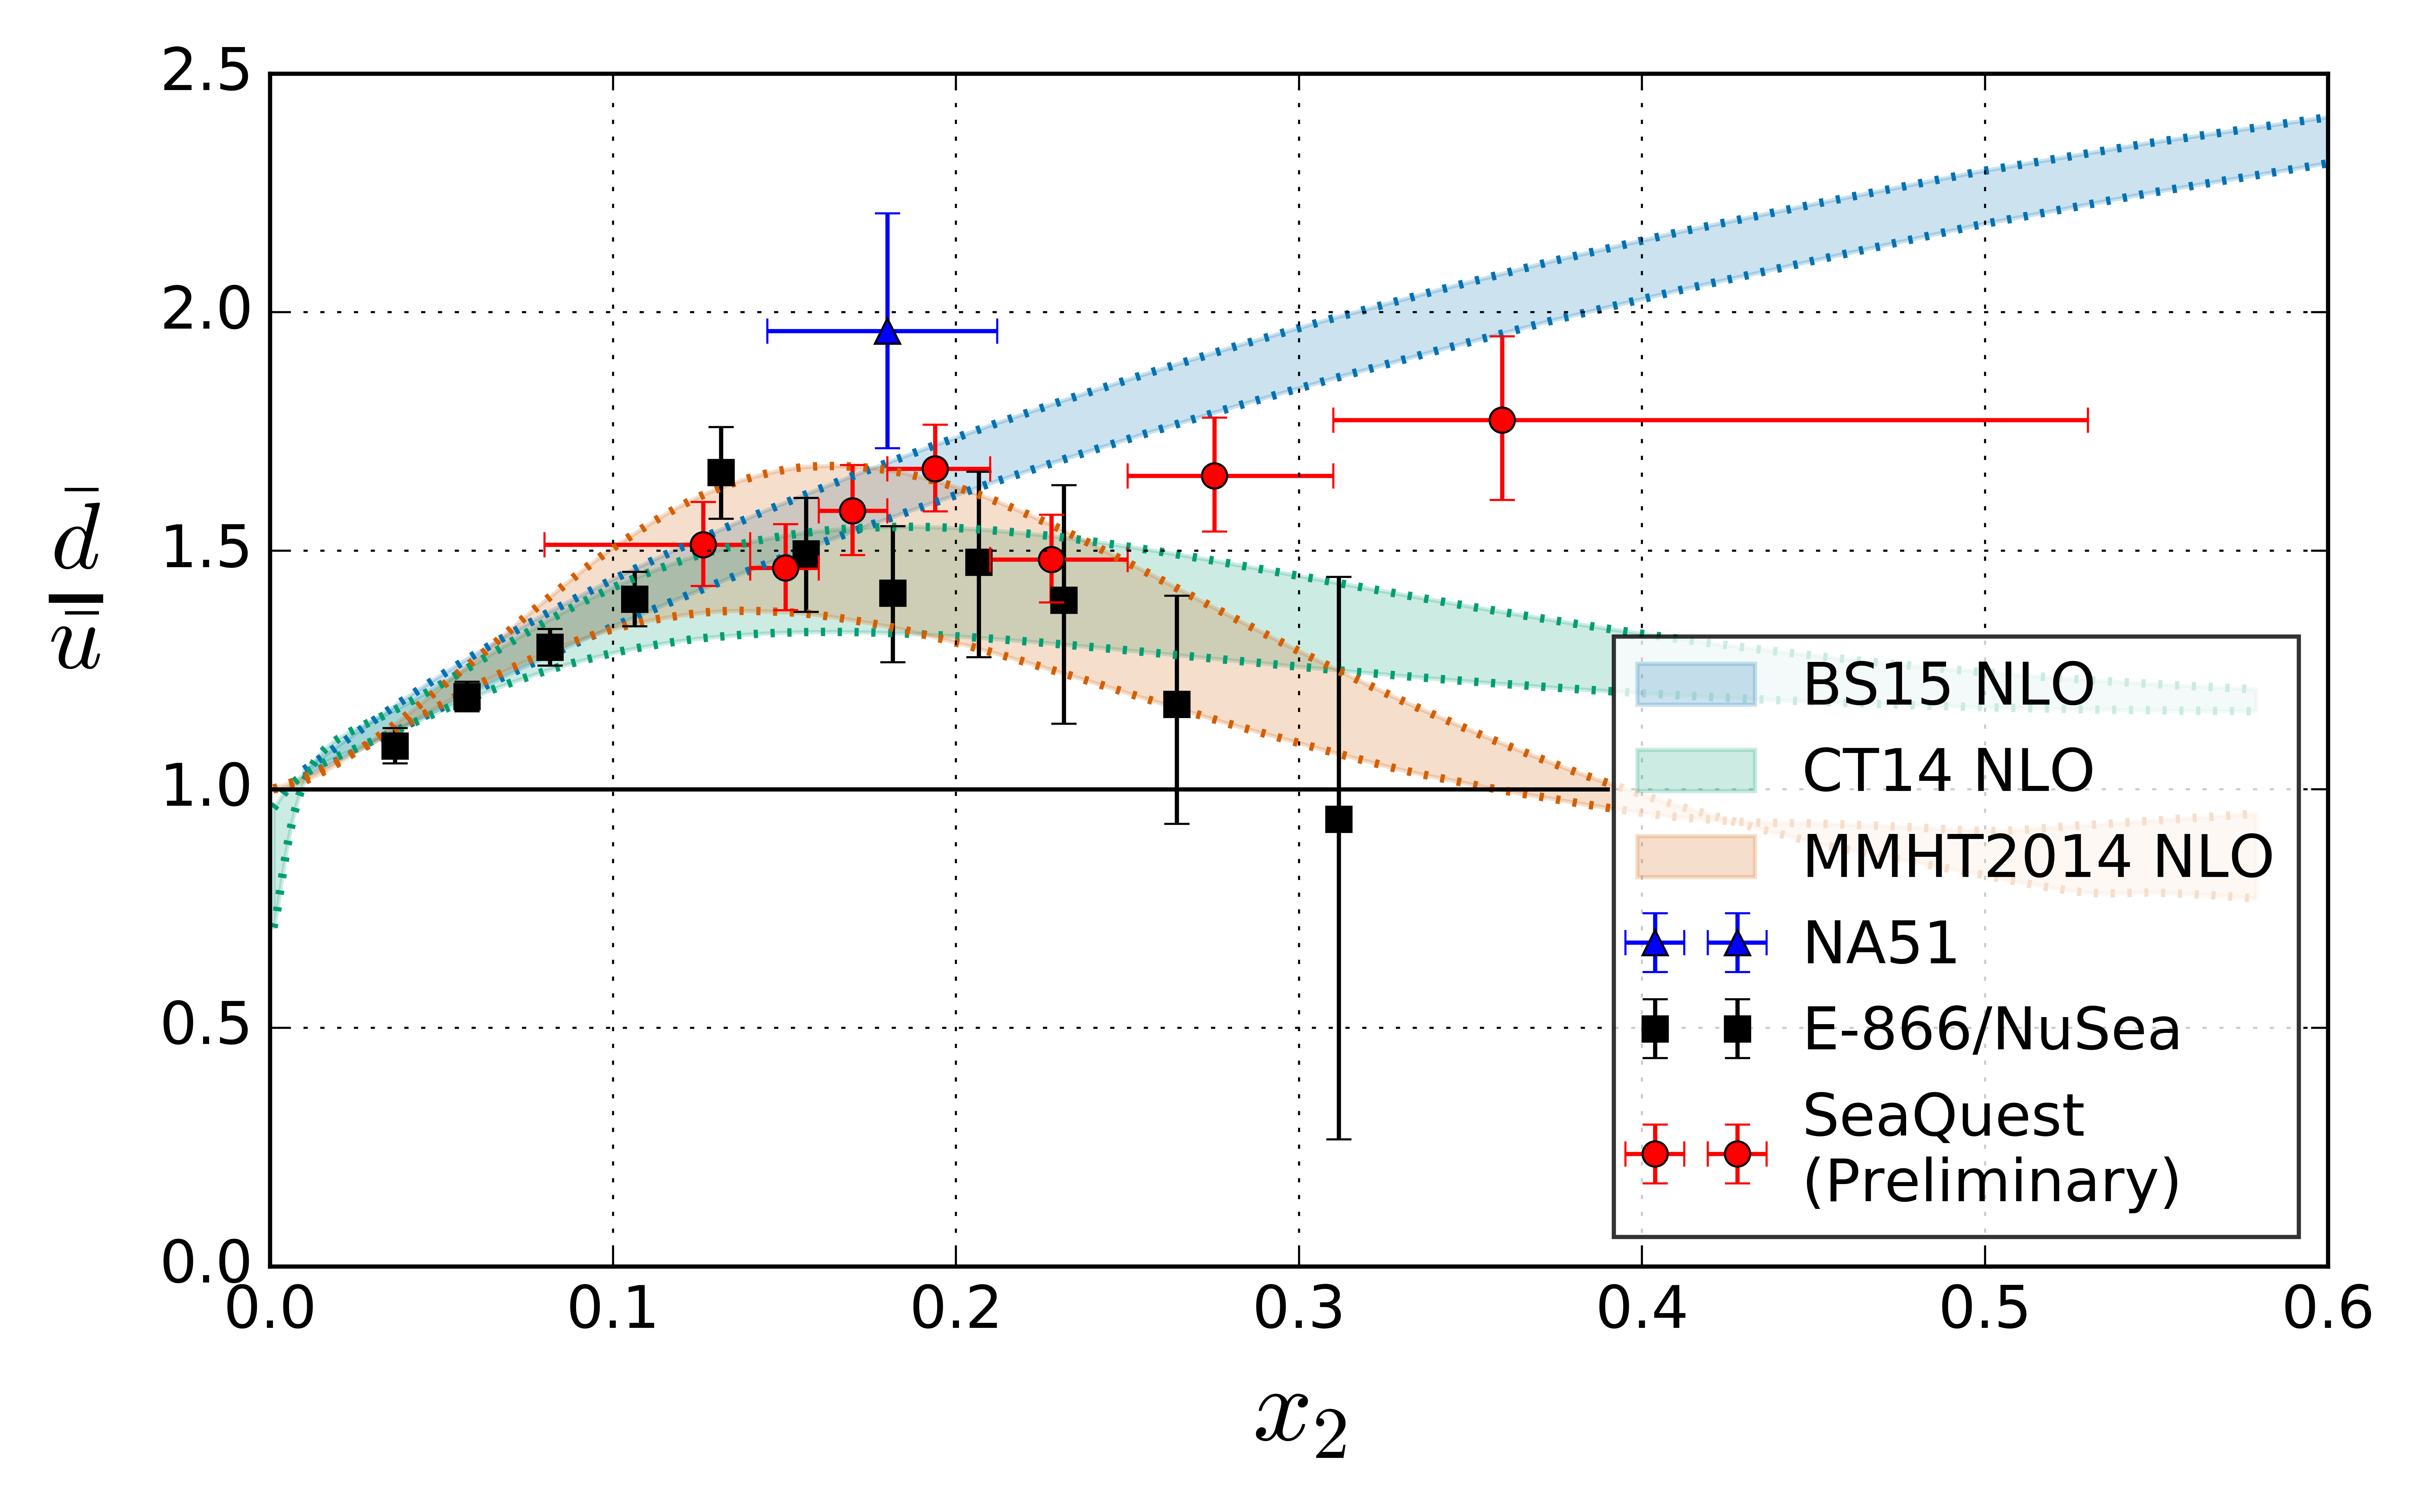
\includegraphics[width=\textwidth]{figures/background/dbar_ubar.png}
	\caption{The measurements and models for the $\dbar/\ubar$ measurement, including the NA51~\cite{Baldit:1994jk}, E-866/NuSea~\cite{PhysRevLett.80.3715}, and (preliminary) SeaQuest experiments, along with the BS15, CT14, and MMHT models.}
	\label{fig:dbar-ubar}
\end{sidewaysfigure}

In the SeaQuest experiment, $\dbar(x)/\ubar(x)$ is to be extracted for the range of approximately $0.1<x_2<0.45$. In the run time since commissioning in 2012, enough data has been analyzed to assemble a preliminary $\dbar(x)/\ubar(x)$ result, which can be seen in Figure~\ref{fig:dbar-ubar}. This measurement and its analysis are being led by Bryan Kerns from the University of Illinois at Urbana-Champaign. Further details regarding this topic can be found in his dissertation and forthcoming publication(s).

\subsection{Meson Cloud Model}

This asymmetry in the nucleon sea was unexpected, though there exists no physical symmetry that does require that $\dbar=\ubar$. The assumption stands that if one were to consider only the primary process of gluons splitting and producing $q\bar{q}$ pairs, then there would be no reason for $d\dbar$ pairs to be preferred to $u\ubar$ pairs. The masses of the $d$ and the $u$ quark are similar enough and are small when compared to the nucleon confinement scale, so they should be produced in equal numbers. Even with perturbative considerations, there does not seem to be an asymmetry in the up/down sea in excess of 1\%~\cite{Ross:1978xk}. There is an excellent discussion by Peng \emph{et al.}~\cite{Peng:1998pa} regarding the possibility of the origin of the $\dbar/\ubar$ asymmetry in the nucleon sea being attributed to virtual mesons.

\begin{wrapfigure}{l}{0pt}
	\centering
	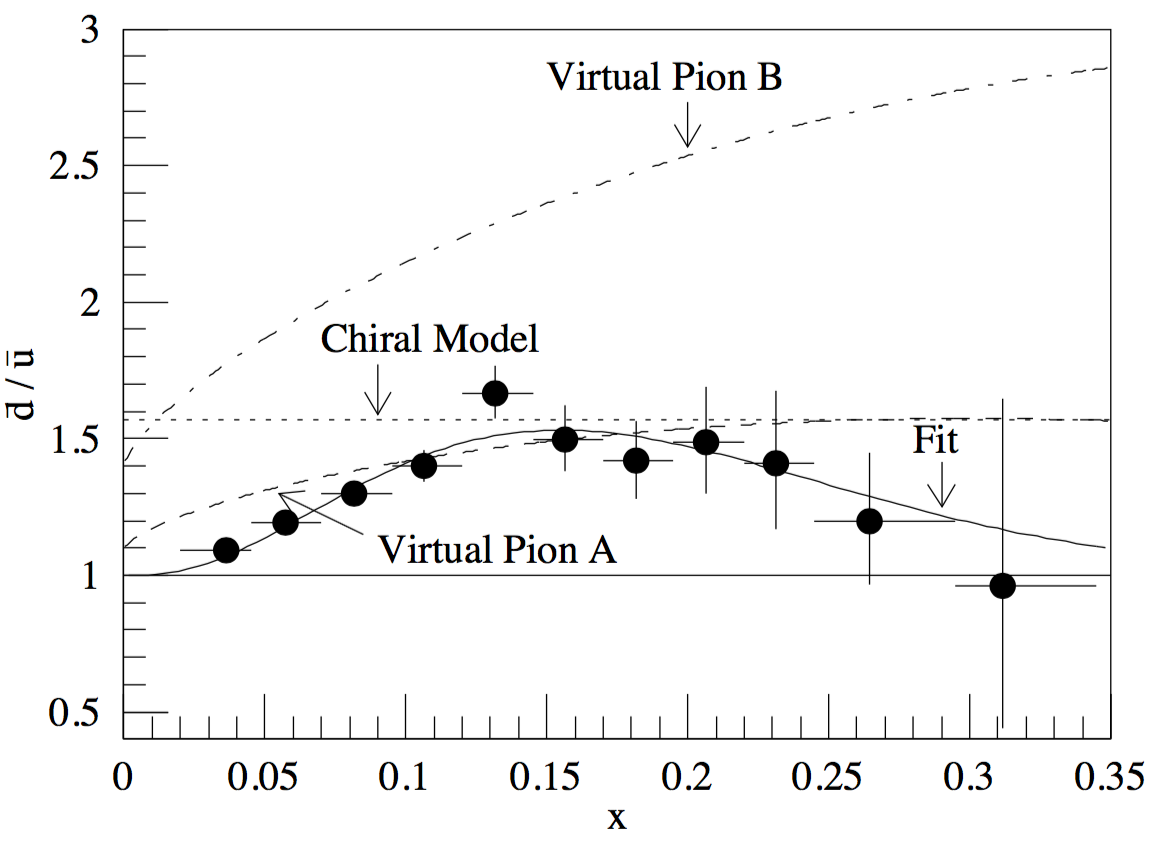
\includegraphics[width=0.4\textwidth]{figures/background/meson-cloud-dbar-ubar.png}
	\caption{The E-866 $\dbar/\ubar$ results compared to three different models~\cite{Peng:1998pa}: a virtual pion model with two different $\pi NN , \pi N\Delta$ dipole form factors~\cite{Kumano:1990mm, Koepf:1995yh} and the chiral model~\cite{Szczurek:1996tp}.}
	\label{fig:pion-model-dbar-ubar}
\end{wrapfigure}
As early as 1983, before a hint of a sea quark flavor asymmetry at NA51, Thomas~\cite{Thomas:1983fh} posited that the non-perturbative interpretation of the measured proton state in terms of its principle meson-baryon Fock components results in a preference for $\dbar>\ubar$. Here, the degrees of freedom being several possible meson-baryon states:
\begin{equation}
|p\rangle_{\text{dressed}} = |p\rangle_{\text{bare}} + a|\pi N\rangle + b|\pi \Delta\rangle + ... .
\end{equation} 
Here, $\pi N$ can be broken into isospin component states $\pi^+ n$ and $\pi^0 p$, with the Clebsch-Gordon coefficients of the states preferring the $\pi^+ n$ state by a factor of two. The $\pi \Delta$ state can be broken down into $\pi^- \Delta^{++}, \pi^0 \Delta^+,$ and $\pi^+ \Delta^0$ states, with their coefficients being 1/2, 1/3, and 1/6, respectively.

These can account for the flavor asymmetry when considering the following: in the $\pi^+ n$ state there exists a $\dbar$ in the ``sea'', in the $\pi^0 p$ state there exist equal number of $\dbar$ and $\ubar$ ($\pi^0=\sqrt{u\ubar+d\dbar}/2$), and in the $\pi^- \Delta^{++}$ case, there exists a $\ubar$ in the ``sea''. The key here is that the $\Delta$ baryon is \unit[294]{MeV} heavier than the $n$ and $p$, making it highly suppressed as compared to the $\pi^+ n$ and $\pi^0 p$ states. This suppression is the basic concept that can account for the $\dbar/\ubar$ asymmetry, as the states in which the $\dbar$ is produced are more likely than the ones in which a $\ubar$ is produced. Formally, one can show~\cite{Szczurek:1993sc} that
\begin{equation}
\int_0^1 dx [\dbar(x)-\ubar(x)] = (2a-b)/3
\end{equation}
and calculations show that the relative probabilities of these configurations $a \approx 2b$~\cite{Koepf:1995yh}. In Figure~\ref{fig:pion-model-dbar-ubar}, the E-866 data for $\dbar/\ubar$ are shown along with three models: two for the virtual pion model with different dipole form factor settings~\cite{Kumano:1990mm, Koepf:1995yh} and one for the the chiral model~\cite{Szczurek:1996tp}. The increased precision and extended $x$-range of $\dbar/\ubar$ as measured by SeaQuest is expected to contribute to the evaluation of these models.

\section{The Nuclear EMC Effect}

Approximately ten years before the NMC experiment's discovery of the $\dbar(x)\neq\ubar(x)$ discovery, the European Muon Collaboration (EMC) at CERN, in 1983, measured the ratios of the structure functions of iron and deuterium over a large kinematic range using the DIS of muons~\cite{Aubert:1983xm}. The result has been repeatedly scrutinized, studied, and confirmed. It was discovered that the structure function of a nucleon bound in a nucleus is fundamentally modified from that of a free nucleon. The nucleus was na\:{i}vely understood as a simple convolution of many nucleons, and that the partonic structure functions of bound and free nucleons should be identical. This assumption was found to not hold against actual measurements, and the observed behavior holds true across all heavy nuclei. This effect can be interpreted as a \emph{modification of quark and gluon distributions in bound nucleons by the nuclear environment}. In this section, the history and collective behavior known as ``The EMC Effect'' will be reviewed, a quantitative A-dependent measure of the effect will be defined, and models that attempt to explain the phenomenon will be discussed. Lastly, the contributions of SeaQuest and previous Drell-Yan experiments to the study of the EMC Effect will be explored.

\subsection{Historical Overview} \label{ssec:emc-history}

\begin{figure}
	\centering
	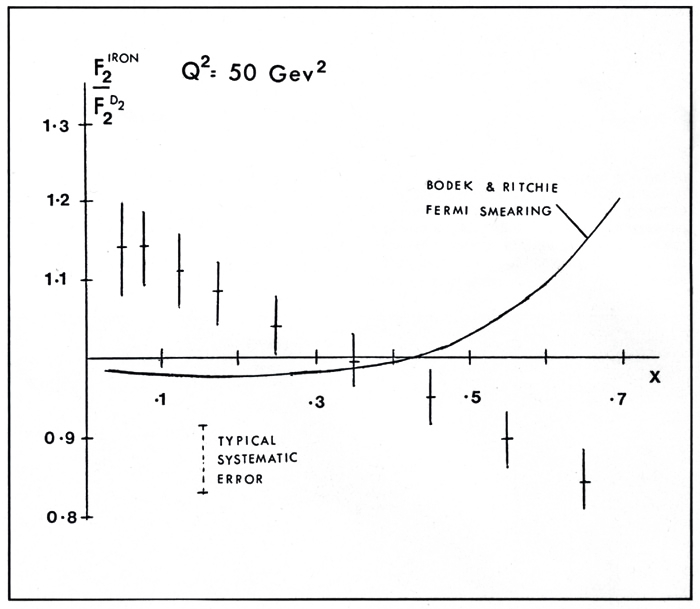
\includegraphics[height=0.35\textheight]{figures/background/emc_effect_original-v2.jpg}
	\caption{The original EMC ratio measurement by the EMC collaboration~\cite{Aubert:1983xm}. Overlaid is the na\:{i}ve, expected ratio taking into account only the Fermi motion of the nucleons in the heavy nucleus.}
	\label{fig:emc-one-naive}
\end{figure}

Unpolarized inclusive lepton scattering is a process that uses an energized lepton to investigate nucleon structure, and it specifically depends on two independent variables: $Q^2$ and Bjorken-$x$ (sometimes referred to as $x_B$, but here left as $x$).
\begin{equation}
Q^2 = -q^2\ \ ;\ \ x = \frac{Q^2}{2 m_p \omega}
\end{equation}
where $q$ is the transferred four-momentum, $x_B$ is the same Bjorken-x scaling variable as is in the PDFs in Section~\ref{sec:pdf} above, $m_p$ is the proton mass, and $\omega$ is the transferred energy in the proton rest frame. At energies of $Q^2>$\unit[2]{(GeV/c)$^2$}, the parton substructure is revealed and the inelastic structure function, $F_2$ is able to be measured. The EMC group extracted the ratio $F_2^{Fe}(x,Q^2)/F_2^{d}(x,Q^2)$, where these are the average bound nucleon structure functions in iron and deuterium. This was done by measuring the DIS \emph{per nucleon cross section ratio}, which can be expressed as~\cite{Halzen:1984mc}:
\begin{equation}
\frac{\sigma^{A_1}/A_1}{\sigma^{A_2}/A_2} = \frac{F_2^{A_1}(x, Q^2)}{F_2^{A_2}(x, Q^2)} \cdot \frac{\left[ 1 + 2\frac{1+\omega^2/Q^2}{R_{A_1}-1}\tan^2\frac{\theta}{2} \right]}{\left[ 1 + 2\frac{1+\omega^2/Q^2}{R_{A_2}-1}\tan^2\frac{\theta}{2} \right]} \approx \frac{F_2^{A_1}(x, Q^2)}{F_2^{A_2}(x, Q^2)}
\end{equation}
where $\theta$ is the lepton scattering angle and $R_A=\sigma^A_L/\sigma^A_T$ is the ratio of the longitudinal to transverse cross section for nucleus A. The A-dependence of $R_A$ will be discussed later, but for now, let us assume that $R$ does not exhibit a nuclear dependence, and the per nucleon cross section ratio therefore approximates nicely to the ratio of the structure functions. For $0.4\gtrsim x\lesssim0.6$ where nucleon Fermi motion effects can be neglected, the expectation was to measure unity, which would indicate that the structure function of a deeply bound nucleon and loosely bound nucleons are identical. With this goal in mind, they chose $^{56}Fe$ and deuterium, as iron is the most tightly bound nucleus at $E^{Fe}_{\text{bind}}=$\unit[8.8]{MeV/nucleon} and deuterium is as close to being a free nucleon as possible while still being a symmetric nuclei ($N=Z=A/2$) with a binding energy of only $E^{d}_{\text{bind}}=$\unit[2.2]{MeV/nucleon}. The reason to perform this experiment is that, if this mearuement showed unity in the regions not affected by Fermi motion, then heavy nuclei could be used to gain a luminosity boost when studying the free nucleon structure functions. Instead, they observed the measured cross-section ration being 1 at $x\approx 0.3$ and then steadily declining to a value of about 0.8 at $x\approx0.7$ (Figure~\ref{fig:emc-one-naive})    

At the time of the measurement was presented, the result astounded the physics community. They could hardly believe that high momentum transfers that were many times larger than the nuclear binding energies that the quark distributions should be altered by the nuclear mean field. This result was confirmed only three months later by the SLAC-MIT-Rochester group that re-examined its data for DIS on steel~\cite{PhysRevLett.50.1431} and found the same behavior, as can be seen in Figure~\ref{fig:emc-e87}. This opened the gates to an enormous amount of activity in both experiment and theory to fully characterize the phenomenon, resulting at present more than 1100 citations of the original EMC publication~\cite{Aubert:1983xm}. \setlength{\columnsep}{28pt} \begin{wrapfigure}{r}{0pt}
	\centering
	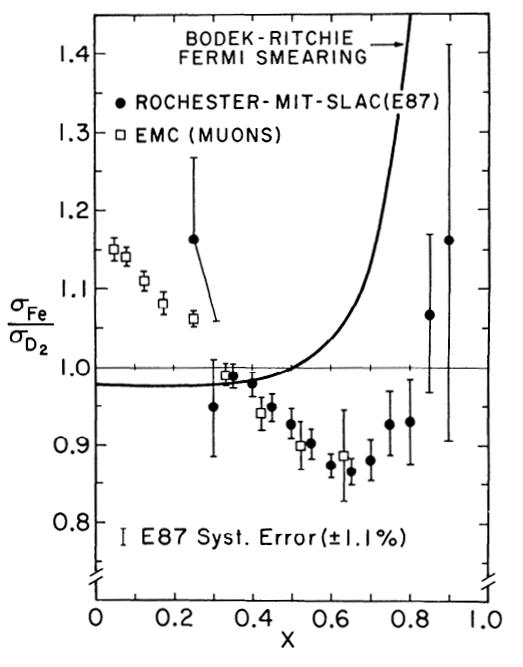
\includegraphics[height=0.35\textheight]{figures/background/SLAC-E87.png}
	\caption{SLAC E-87 was quick to report its own finding months later confirming EMC's observation~\cite{PhysRevLett.50.1431}.}
	\vspace{-20pt}
	\label{fig:emc-e87}
\end{wrapfigure} The compendium of experimental data and theory papers have been discussed in great detail in the excellent review papers by Geesaman~\cite{Geesaman:1995yd} in 1995 and Norton~\cite{norton:emc-review} in 2003. As such, I will only summarize the main theoretical ideas and the most prominent interpretation of the effect. A visual summary of EMC data can be found in Figure~\ref{fig:emc-all-targ} where data from EMC~\cite{Aubert:1983xm}, SLAC~\cite{Arnold:1983mw, Gomez:1993ri}, BCDMS~\cite{Benvenuti:1987az}, NMC~\cite{Amaudruz:1991nw}, and HERMES~\cite{Ackerstaff:1999ac} is plotted for nine different targets.

\begin{figure}
	\centering
	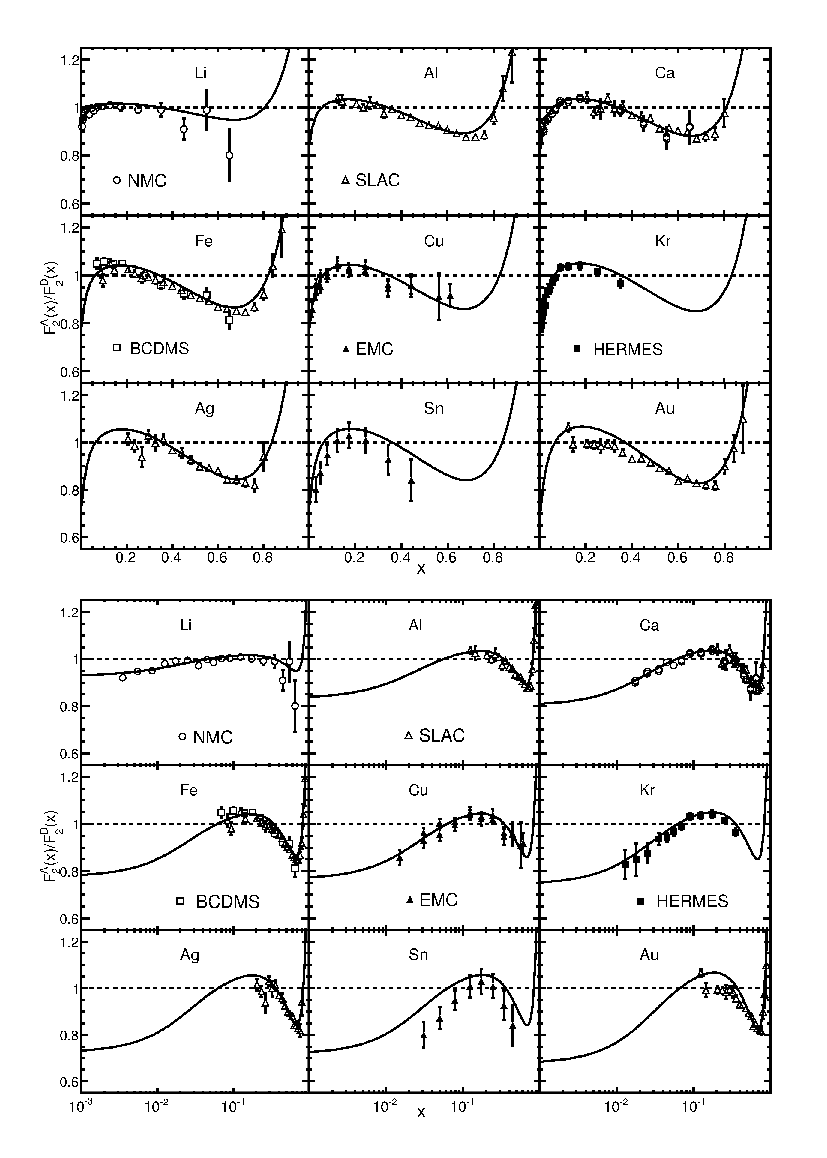
\includegraphics[height=0.9\textheight]{figures/background/emc-all-targ.eps}
	\caption{A compilation of data regarding the measurement of $F^A_2/F_2^D$ for nine different heavy targets with an overlaid fit by Chen et al.~\cite{Chen:2013oga}.}
	\label{fig:emc-all-targ}
\end{figure}

\subsection{\texorpdfstring{Universal $x$-dependence}{Universal x-dependence}}

The SLAC E139 experiment provides very precise information for the high-$x$ range ($x>0.2$) for many nuclei. The high-energy electron DIS data from SLAC E61~\cite{Stein:1975yy} and HERMES~\cite{Ackerstaff:1999ac} experiments along with the muon DIS data from NMC~\cite{Amaudruz:1991nw} supplements this with the very low-$x$ range. Finally, the more recent data from JLAB-E03103~\cite{Seely:2009gt} that uses a relatively low energy beam (\unit[5.8]{GeV}) provides data for the high-$x$ Fermi motion area ($0.85<x<0.95$). These together help to paint a full characteristic picture of the $x-$dependence of this $\sigma^A/\sigma^d$ ratio, which has been found to be universal for all $A>2$. A visualization of some of this data for carbon and nitrogen  the measurement up into four qualitative regions of this ratio can be seen in Figure~\ref{fig:emc-regions}.
\begin{figure}
	\centering
	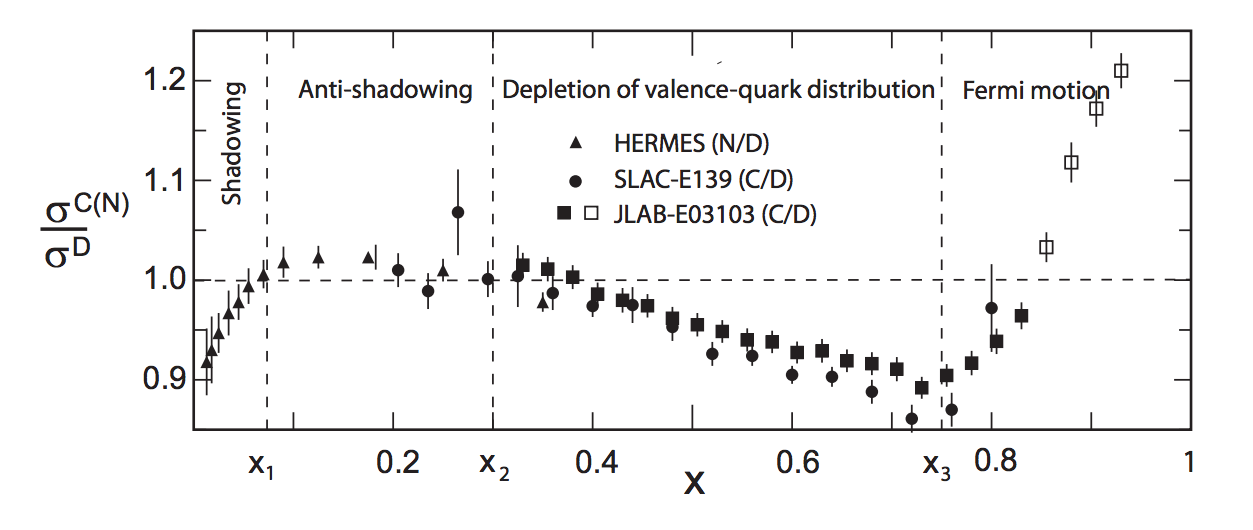
\includegraphics[width=\textwidth]{figures/background/emc-regions.png}
	\caption{The ratio of $\sigma^{C(N)}/\sigma^d$ covering nearly the entire $x\in[0,1]$ interval~\cite{Rith:2014tma}. The four qualitative regions are denoted by roughly chosen boundaries $x_1, x_2, x_3$ (not to be confused with the beam and target $x_1$ and $x_2$ used in the rest of this paper).}
	\label{fig:emc-regions}
\end{figure}
\begin{itemize}
	\item $\mathbf{0<x\lesssim0.06:}$ The ``shadowing'' region where the ratio is less than unity and decreasing as $x\rightarrow0$. The dominant contribution to the cross section in this kinematic regime is from sea quarks.
	\item $\mathbf{0.06\lesssim x \lesssim 0.3:}$ The (perhaps poorly named) ``anti-shadowing'' region exhibits a very slight rise of the ratio above unity. In general, this range of values represents only a transition region between its two bookending effects.
	\item $\mathbf{0.3\lesssim x \lesssim 0.8:}$ The ratio becomes significantly smaller than unity, decreasing with increasing $x$. This is of key focus for this paper, and this region is what is generally referred to as the \emph{``EMC Effect''}~\cite{Geesaman:1995yd} as it is the only part of the phenomenon that is not fully understood.  As far as DIS goes, the sea quark contribution is essentially negligible, given the current understanding of quark PDF's, and the behavior is dominated by valence quark distributions.
	\item $\mathbf{0.8\lesssim x < 1:}$ The ratio increases rapidly with increasing $x$. This is dominated by a kinematic effect of the free nucleon cross section vanishing as $x\rightarrow1$. It is also due to the effect of Fermi motion of the bound nucleons in the nucleus.
\end{itemize}

\subsection{Nuclear Dependence of R}

It was stated in section~\ref{ssec:emc-history} that the per nucleon cross section ratio only reduces to the ratio of structure functions in the case that $R=\sigma_L/\sigma_T$ is A-independent. This particular measurement was the focus of experiments SLAC-E140~\cite{PhysRevLett.61.1061, Dasu:1993vk}, NMC~\cite{Arneodo:1996qe}, and HERMES~\cite{Ackerstaff:1999ac}. A re-analysis of all SLAC data with improved corrections~\cite{Dasu:1993vk} showed that the difference in $R$ between iron and deuterium is consistent with zero ($R_{Fe}-R_d = 0.001 \pm 0.018 (\text{stat}) \pm 0.016 (\text{sys.})$), and that there are no significantly different spin-0 constituents or higher twist effects in nuclei as compared to free nucleons. Later on, results from HERMES corroborated these findings. The ratio of $R_A/R_d$ were derived from the NMC and SLAC results for $\Delta R = R_A - R_d$ and reported an averaged value of $R_A/R_d = 0.99 \pm 0.03$, providing further agreement on the A-independence of $R$.

A recent study by Guzey et al.~\cite{Guzey:2012yk} looked to data from SLAC E139, BCDMS, and EMC to examine the impact of $R$ on the extraction of $F_2^A/F_2^d$ and $F_1^A/F_1^d$ from $\sigma^A/\sigma^d$ data. They demonstrate the presence of a small but non-zero difference between $R$ for nuclei and free nucleons. While this does appear to effect the extraction of the nuclear enhancement in the ratio of the $F_1^A/F_1^d$, the extraction of $F_2^A/F_2^d$ appears to remain unaffected. As such, this thesis assumes that it is safe to assume that $\sigma^A/\sigma^d \approx F_2^A/F_2^d$.

\subsection{$Q^2$ Dependence of EMC Effect}

\begin{figure}[!b]
	\centering
	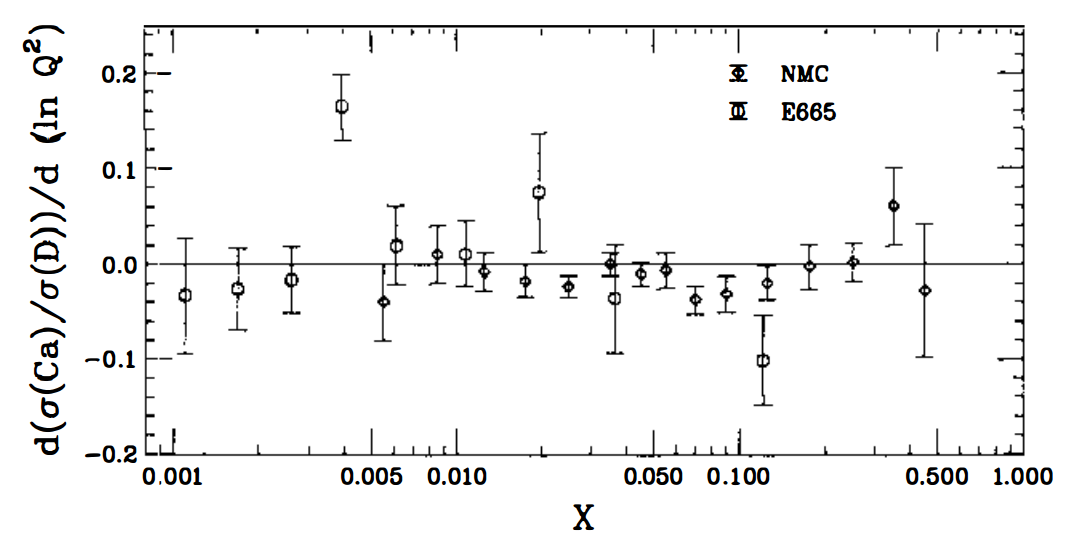
\includegraphics[width=0.8\textwidth]{figures/background/emc-q2-dep.png}
	\parbox{4.5in}{\caption{Measurements of the change in the $\sigma^{Ca}/\sigma^d$ ratio with respect to $\ln Q^2$  over a broad range of $x$~\cite{Geesaman:1995yd}.}
		\label{fig:emc-q2-dep}}
\end{figure}
It is important when investigating structure functions and quark/gluon distributions to pay attention to the $Q^2$ sensitivity of the measurements. Nuclear structure functions can be directly interpreted as parton distributions only if $Q^2$ is large enough to precisely define the light-cone direction and reduce higher-twist contributions. The first condition places a restriction on $x^2/Q^2$ and is usually well satisfied, even at relatively low values of $x$ and $Q^2$. However, the value of the higher-twist terms is under little theoretical control, and these terms can have specific nuclear dependences. 

Experimentally, the verdict was very clear from the agreement between muon and electron DIS data that any $Q^2$ dependence must be very small since, at the same value of $x$, their average $Q^2$ differs by more than an order of magnitude. The lack of $Q^2$ dependence can be seen in Figure~\ref{fig:emc-q2-dep} which shows the derivative of DIS cross section with respect to $\ln Q^2$ over a broad range of $x$, combining NMC and E665 data for calcium~\cite{Geesaman:1995yd}.  \emph{This absence of any observable dependence of the ratio on $Q^2$ justifies the usual practice of combining all the $Q^2$ data at a fixed $x$-value to display the $x$-dependence of the ratio}. The only measurement that seems to refute this conclusion is a measurement of $\sigma^{Sn}/\sigma^C$ by NMC which observes a statistically significant, yet small $Q^2$ dependence at small values of $x$ ($x\lesssim 0.06$)~\cite{Arneodo:1996qe}. Due to a large amount of evidence to the contrary along with the fact that SeaQuest is only sensitive to $x\gtrsim0.08$, this paper will move forward with the understanding that there is no $Q^2$ dependence in this ratio measurement. As such, this paper will frequently abbreviate such expressions:
\begin{equation}
\frac{F_2^A(x, Q^2)}{F_2^d(x, Q^2)} \rightarrow \frac{F_2^A(x)}{F_2^d(x)}\ \ \ ;\ \ \ \frac{2}{A}\frac{\sigma^A(x, Q^2)}{\sigma^d(x, Q^2)} \rightarrow \frac{2}{A} \frac{\sigma^A(x)}{\sigma^d(x)}
\end{equation}
when in reality it is only the ratio that is $Q^2$-independent.

\subsection{Shadowing}\label{sec:shadowing}

Even though the ``shadowing'' region of the EMC effect ($x\lesssim 0.06$) is outside of the kinematic acceptance of the SeaQuest experiment ($x\gtrsim0.08$), it is certainly worth briefly discussing this interpretation. This term ``shadowing'' has been introduced to explain the reduction of the nuclear cross sections in photoproduction, but in this particular case, has also been used in discussing very low-$x$ modifications to the nuclear cross section in DIS. 

The generally accepted explanation for this modification is that the parton distributions in bound nucleons actually \emph{remain unchanged} compared to those in free nucleons. In the rest frame of the \emph{nucleus}, the nuclear effect is attributed to the modification of the interaction of the virtual photon with the atomic nucleus by fluctuations of the virtual photon into quark-antiquark pairs. This pair then interacts with the nucleus via the strong interaction instead of electromagnetically. As a result of this increase in strength, the interaction no longer proceeds incoherently with all the rest of the nucleons, but \emph{preferentially with those at the front surface}. The other nucleons in the ``shadow'' of the nucleons in front are much less likely to interact, and thereby do not (or much less) contribute to the cross section. As a result, when calculating the per nucleon cross section ratio $\frac{\sigma^A/A}{\sigma^d/2}$ and the deuteron essentially has the same cross section as the heavy nucleus (in this specific regard), then the ratio value will be suppressed.  

Quantitatively, this behavior will occur when the $q\bar{q}$ pair fluctuation exists for longer than the mean free path of the pair in a nucleus (distance between nucleons). The fluctuation length behaves as $\Delta d \approx 1/Mx$ where $M$, the effective mass of the $q\bar{q}$ pair is approximately \unit[1.1]{GeV}~\cite{Kopeliovich:2012kw}, yielding a fluctuation distance of $\Delta d \approx \unit[0.2]{fm}/x$. This becomes larger than the mean free path $L\simeq\unit[2.5]{fm}$ when $x\lesssim 0.08$.

\subsection{Fermi Motion}

\begin{wrapfigure}{r}{0pt}
	\centering
	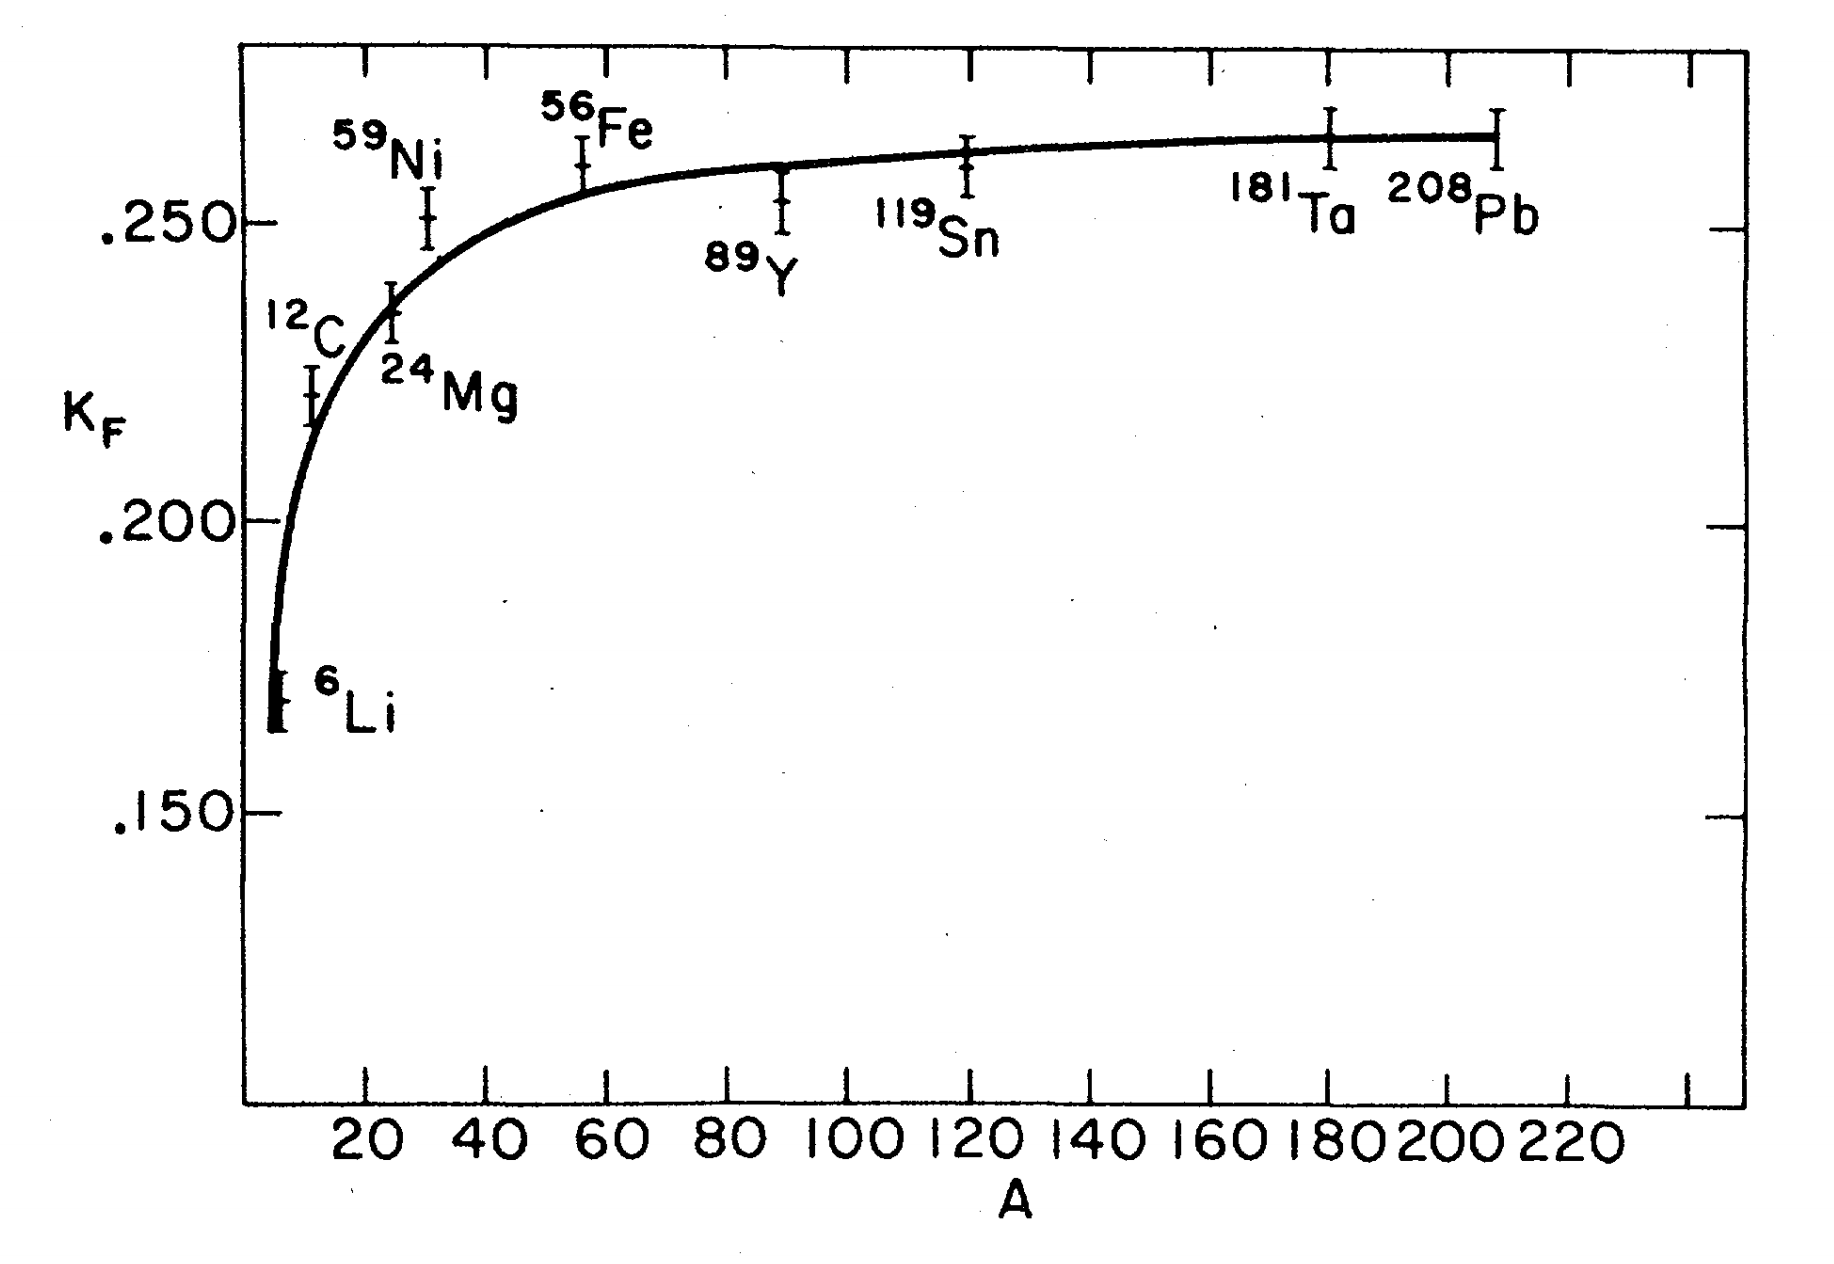
\includegraphics[width=0.45\textwidth]{figures/background/fermi-momentum.png}
	\caption{The Fermi momenta $K_F$ (in GeV) for various nuclei of atomic weight A~\cite{PhysRevD.23.1070}.}
	\vspace{-20pt}
	\label{fig:fermi-momentum}
\end{wrapfigure}
One of the more striking features of the $F_2^A(x)/F_2^d(x)$ is the sharp rise in the ratio value at high-$x$ ($0.8\nobreak\lesssim\nobreak x\nobreak\lesssim\nobreak1$). This feature arises as a result of the quantum mechanical principle of Fermi motion, which arises from the confinement of nucleons within the nucleus. If one considers the uncertainty principle inherent in all wave-like systems, $\sigma_x \sigma_p \geq \frac{\hbar}{2}$, there is a direct effect on the momentum distribution of nucleons when one considers the spatial localization of bound nucleons in a nucleus. For example, the nucleons in a tightly bound nucleus (like iron) must have a more precise spatial localization (smaller $\sigma_x$) than a nucleon in a more loosely bound nucleus (such as the deuteron). As a result, the magnitude of momentum variations will be greater in the case of iron than in the deuteron (an effect sometimes called ``Fermi smearing''). The magnitude of the Fermi momenta of several nuclei can be found in Figure~\ref{fig:fermi-momentum}.

In the extreme case of a free nucleon (which deuterium is chosen to approximate as best as possible), there exists no Fermi motion, as the nucleon is unbound. As a result, the $F_2$ structure function must vanish as $x\rightarrow1$ as it becomes very unlikely that a single quark will possess a large fraction of the momentum of the free nucleon without the help of quantum mechanical fluctuations and Fermi smearing. In the case of the deuteron, though, there is still some Fermi motion, as it still consists of two bound nucleons. Bodek and Ritchie were among the first to lay out a model for comparing this effect and how it would differ between different nuclei~\cite{PhysRevD.23.1070}.  The model of how this would affect the structure function ratio is seen on the original EMC plot in Figure~\ref{fig:emc-one-naive}, given no other nuclear effects (such as the EMC Effect).

As is the case with shadowing, this regime is far beyond the kinematic acceptance of SeaQuest to measure. There is still good reason to believe that, whatever the cause of the EMC effect, it likely overlays the effect of Fermi motion, which, depending on the model, can affect the ratio measurement above $x\approx0.5$. Even with this estimate, there are very few SeaQuest statistics at this $x$-range.

\subsection{A-dependence of EMC Effect Slope}

\begin{table}
	\centering
	\ra{1.2}
	\setlength{\tabcolsep}{2em}
	\begin{tabular}{@{}lllll@{}}\toprule
		Nucleon & & $dR_{EMC}/dx$~\cite{Seely:2009gt} & $dR_{EMC}/dx$~\cite{Gomez:1993ri} & $dR_{EMC}/dx$ (comb.) \\ \midrule    
		$^2H$ & &                                      &                                   & -0.10$\pm$0.05~\cite{Griffioen:2015hxa} \\
		$^3He$ & & -0.070$\pm$0.029     &                                 & -0.070$\pm$0.029 \\
		$^4He$ & & -0.199$\pm$0.029        & -0.191$\pm$0.061   & -0.191$\pm$0.026 \\
		$^9Be$ & & -0.271$\pm$0.029         & -0.207$\pm$0.037  & -0.243$\pm$0.023 \\
		$^{12}C$ & & -0.280$\pm$0.029    & -0.318$\pm$0.040  & -0.292$\pm$0.023 \\
		$^{27}Al$ & &                                 & -0.325$\pm$0.034  & -0.325$\pm$0.034 \\
		$^{40}Ca$ & &                                 & -0.350$\pm$0.047 & -0.350$\pm$0.047 \\
		$^{56}Fe$ & &                                 & -0.388$\pm$0.032 & -0.388$\pm$0.032 \\
		$^{108}Ag$ & &                                 & -0.496$\pm$0.051 & -0.496$\pm$0.051 \\
		$^{197}Au$ & &                                 & -0.409$\pm$0.039 & -0.409$\pm$0.039 \\ \bottomrule        
	\end{tabular}
	\caption{Measured EMC slopes $dR_{EMC}/dx$ for $0.35\leq x \leq 0.7$~\cite{Piasetzky:2011zz}.}
	\label{tab:emc-slopes}
\end{table}

Precise measurements of $R_{EMC}=(F_2^A/A)/(F_2^d/2)$ for various nuclei, from $^3He$ to $^{197}Au$ have been analyzed, and the intermediate-to-high $x$ region ($0.35<x<0.7$) shows a declining behavior that can be fit with a line. The slope of this line has become the focus of study when attempting to interpret the EMC effect, as this slope ($dR_{EMC}/dx$) exhibits a significant A-dependence. The magnitudes of the slopes appear to increase with increasing $A$. The table of values of $dR_{EMC}/dx$ for various nuclei can be found in Table~\ref{tab:emc-slopes}.

\begin{wrapfigure}{l}{0pt}
	\centering
	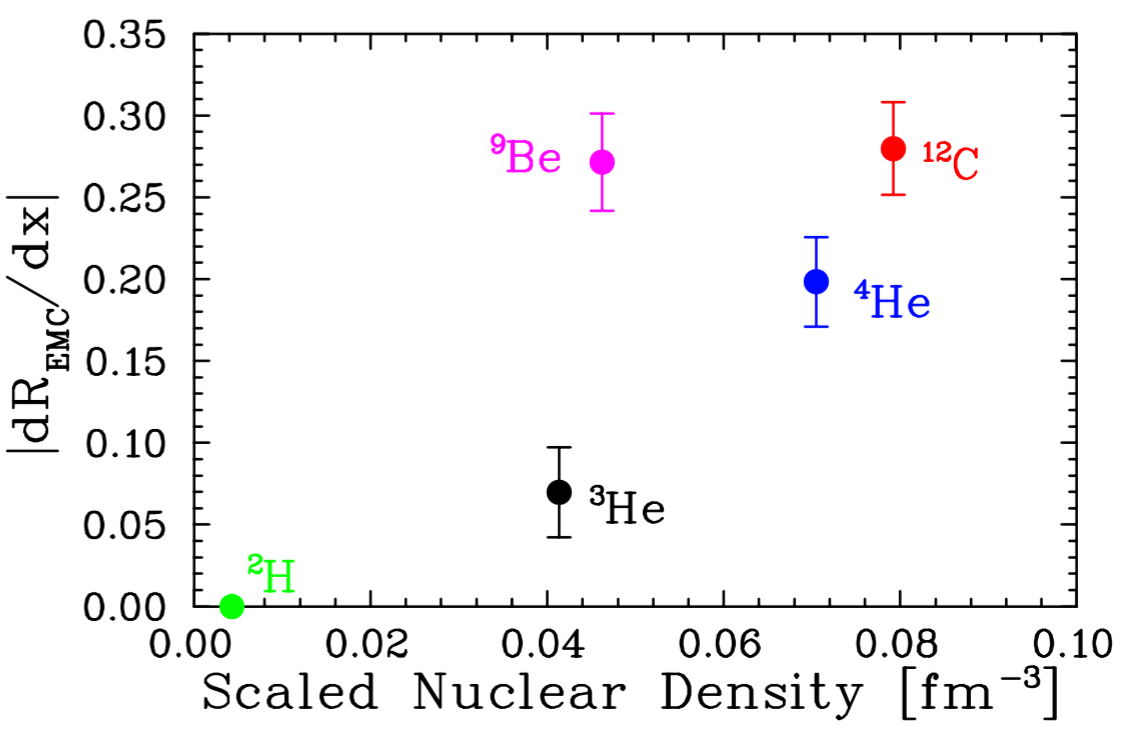
\includegraphics[width=0.4\textwidth]{figures/background/emc-vs-density.png}
	\caption{The slopes of the EMC ratio for $0.35<x<0.7$ vs the average nuclear density scaled by $(A-1)/A$~\cite{Seely:2009gt}.}
	\label{fig:emc-slope-vs-density}
\end{wrapfigure}
The initial attempt at understanding this was to interpret it as some effect of nuclear density. Since the effect of nuclear density on a given nucleus is due to the presence of the other ($A-1$) nucleons, the slope $|dR_{EMC}/dx|$ was plotted against the average nuclear density scaled down by a factor of $(A-1)/A$ in order to remove the struck nucleon’s contribution to the average nuclear density. The result for light nuclei was shown by Seely \emph{et al.} to have an interesting result, as is seen in Figure~\ref{fig:emc-slope-vs-density}. The most notable result was a definite overall trend with $^9Be$ representing a significant outlier. It has been theorized that $^9Be$ is an outlier due to its nuclear structure resembling two $\alpha-$particles ($^4He$ nuclei) with an extra neutron. This would mean that perhaps it is not the average nuclear density, but the \emph{local} nuclear density or density about the struck nucleon. There is still a missing piece needed to represent this density.



\subsection{$x>1$ Plateaus and Short Range Correlations}

What has recently spurred renewed interest in the EMC effect and its possible true origin is a series of measurements by JLAB of election DIS cross section ratios where $x>1$. In this kinematic space, the cross section from a free nucleon vanishes, but persists for the deuteron. It may not at first make sense that measurements can be made in this high $x$, but it is accessible. Such a behavior is interpreted as the manifestation of short-range nucleon-nucleon correlations (three-nucleon correlations for $x>2$). These short-range correlations happen when two (or three) nucleons happen to get very close to each other and experience a large repulsive Coulomb force, resulting in the nucleons moving apart from each other with high \emph{individual} momentum, but low \emph{combined} momentum.

\begin{figure}[!tbp]
	\centering
	\begin{minipage}[b]{.4\textwidth}
		\centering
		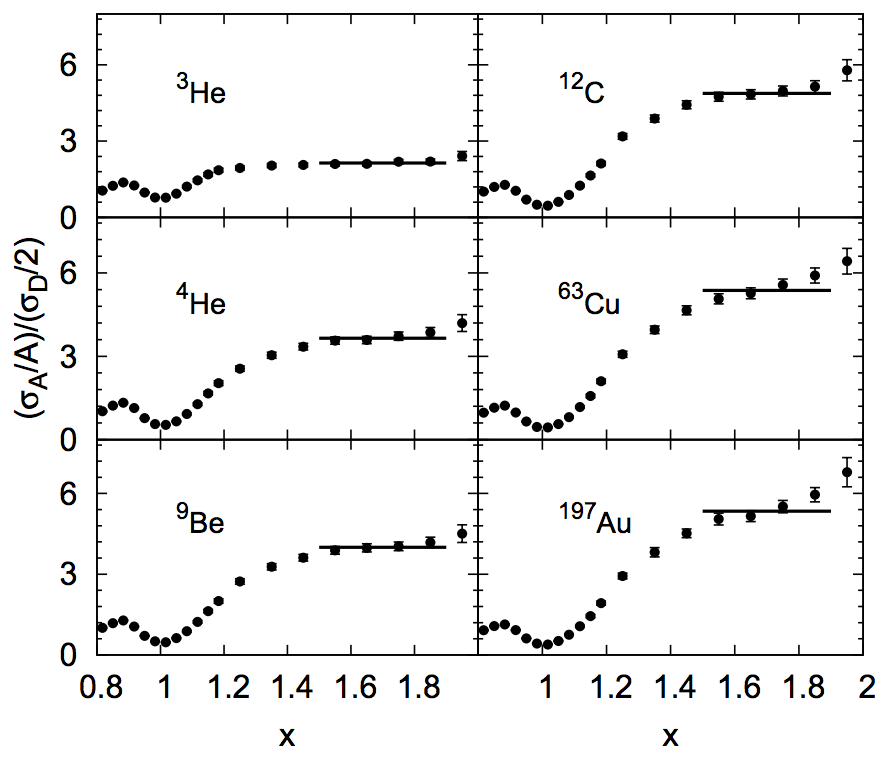
\includegraphics[height=0.3\textheight]{figures/background/nn-src-plateau.png}
		\caption{Per nucleon cross section ratios vs $x$ at $0.8<x<2$ as measured by JLAB-E02019 with a line fit to the ``plateau'' regions at $1.5<x<1.9$~\cite{Fomin:2011ng}.}
		\label{fig:nn-src-plateau}
	\end{minipage}%
	\hfill
	\begin{minipage}[b]{.4\textwidth}
		\centering
		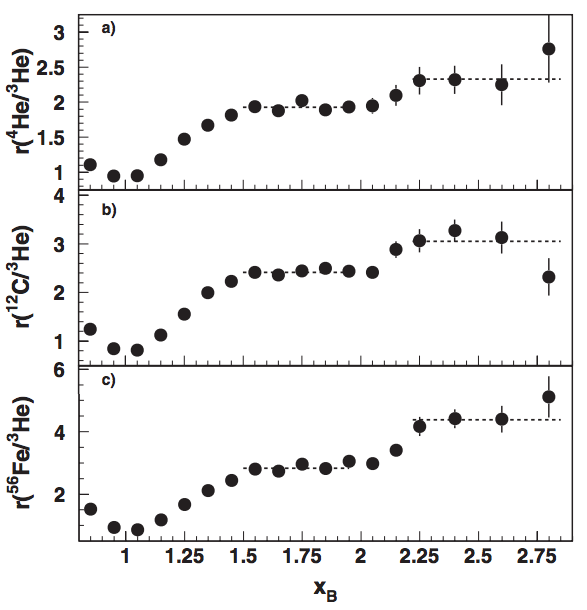
\includegraphics[height=0.3\textheight]{figures/background/CLAS-nnn-src-ratio.png}
		\caption{Per nucleon cross section ratios vs $x$ at $0.75<x<3$ as measured by CLAS with a line fit to the ``plateau'' regions  at $2.25<x<2.8$~\cite{PhysRevLett.96.082501}.}
		\label{fig:nnn-src-plateau}
	\end{minipage}
\end{figure}

The JLAB-E02019 experiment~\cite{Fomin:2011ng} measured cross section ratios for $^3He$, $^4He$, $Be$, $C$, $Cu$ and $Au$ to deuterium. One can see in the results shown in Figure~\ref{fig:nn-src-plateau} that the cross section ratios of $^4He/D$, $C/D$ and $Cu/D$ rise with $x$ until the value plateaus at $x \approx 1.4 - 1.5$. The key observation with these plateaus is that the ratio value at this plateau increases with $A$. Such behavior was already observed with less accuracy by an experiment at SLAC~\cite{Frankfurt:1993sp}, and a similar pattern can be seen in the CLAS experiment which compared nuclear cross sections to tritium ($^3He$)~\cite{PhysRevLett.96.082501}. Here the measurements extend up to $x=3$ and an indication of a second plateau is observed for $2.25<x<2.8$ (Fig.~\ref{fig:nnn-src-plateau}). 

The variable $a_2(A/d)$ is introduced here as the ratio (in the plateau range) of the per-nucleon inclusive ($e,e^\prime$) cross sections for two nuclei. This value can be interpreted as the \emph{ratio of probabilities to find high-momentum nucleons in those two nuclei}~\cite{PhysRevLett.106.052301}. High-momentum nucleons were recently shown to arise primarily from nucleon-nucleon short range correlations, which is when two nucleons' wave functions overlap briefly, causing them to have high relative momentum but low combined momentum (relative to the $\sim\unit[400]{MeV}$ Fermi motion)~\cite{PhysRevLett.100.162503}.  Thus, this $a_s(A/d)$ ratio is called the ``Short Range Correlation (SRC) Scale Factor''\footnote{More specifically, it is called the 2N-SRC scale factor, as there is a three-nucleon scale factor for cross section ratios with respect to tritium.}  The current known values for the SRC scale factors are shown in Table~\ref{tab:a2-src}. The variables $a_2(A/^3He)$ and $a_3(A/^3He)$ is also defined for first and second plateau ranges, respectively, but are not emphasized here.

\begin{table}
	\centering
	\ra{1.2}
	\setlength{\tabcolsep}{2em}
	\begin{tabular}{@{}lllll@{}}\toprule
		Nucleon & & $a_2(A/^3He)$~\cite{Egiyan:2005hs} & $a_2(A/d)$~\cite{PhysRevLett.106.052301} & $a_2(A/d)$~\cite{Fomin:2011ng} \\ \midrule    
		$^2H$ & &     0.508$\pm$0.025         & 1                                 &  1 \\
		$^3He$ & & 1                                  & 1.97$\pm$0.10        & 2.13$\pm$0.04 \\
		$^4He$ & & 1.93$\pm$0.14            & 3.80$\pm$0.34      &  3.60$\pm$0.10 \\
		$^9Be$ & &                                        &                               & 3.91$\pm$0.12 \\
		$^{12}C$ & & 2.41$\pm$0.17            & 4.75$\pm$0.41          & 4.75$\pm$0.16  \\
		$^{56}Fe$ & & 2.83$\pm$0.18           & 5.58$\pm$0.45        &  \\
		$^{63}Cu$ & &                                 &                                 & 5.21$\pm$0.20 \\
		$^{197}Au$ & &                                 &                                 & 5.16$\pm$0.22 \\ \bottomrule        
	\end{tabular}
	\caption{Measured SRC scale factors, as measured by CLAS~\cite{Egiyan:2005hs} and JLAB E02-019~\cite{PhysRevLett.106.052301, Fomin:2011ng}.}
	\label{tab:a2-src}
\end{table}

\begin{wrapfigure}{r}{0pt}
	\centering
	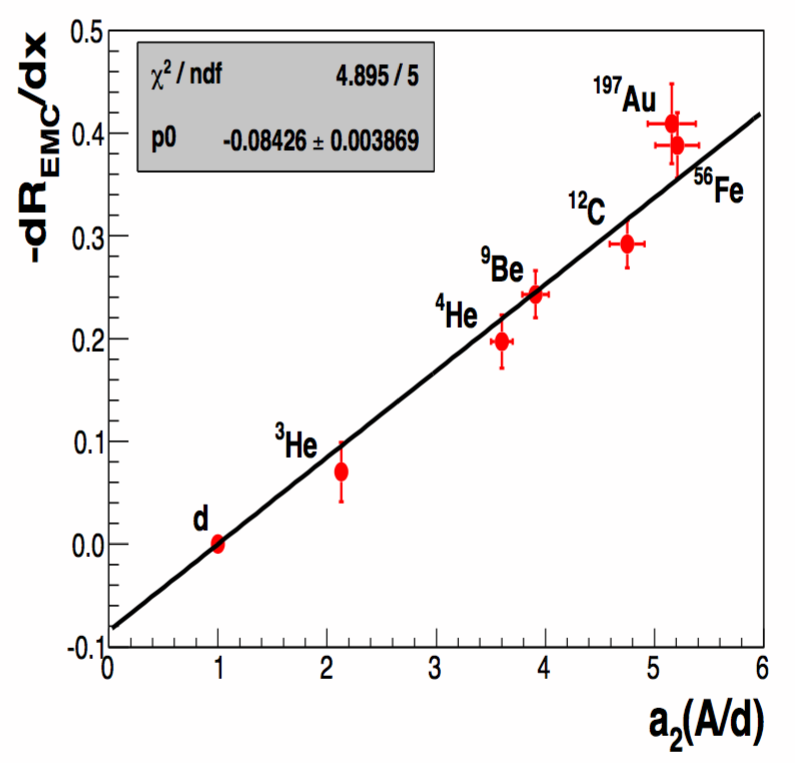
\includegraphics[width=0.5\textwidth]{figures/background/emc-a2.png}
	\caption{The EMC slopes plotted agains the 2N-SRC scale factors~\cite{Hen:2012fm}. The fit is constrained to go through deuterium at (1,0).}
	\label{fig:emc-a2}
\end{wrapfigure}
It was first posited by Higinbotham \emph{et al.}~\cite{Higinbotham:2010ye} that the magnitude of the EMC effect in a nucleus $A$ is related to the measured SRC scale factor of the same nucleus if both are taken relative to deuterium. In Figure~\ref{fig:emc-a2}, the EMC slopes from Table~\ref{tab:emc-slopes} are plotted agains the SRC scale factors from Table~\ref{tab:a2-src} to exhibit a strong correlation indicated by the straight line. It would seem unlikely that this is coincidental, and it can therefore be asserted with some confidence that the EMC effect seen in the valence quarks is largely due to these 2N-SRC~\cite{Rith:2014tma}.

There is a future study planned at JLAB to test this 2N-SRC - EMC effect connection, experiment E12−11−107, which has been approved to run as part of their \unit[12]{GeV} program. The experiment will study the structure function of high-momentum nucleons in deuterium by performing electron DIS from nucleons in deuterium and identifying nucleons that are knocked out \emph{backwards} towards the direction that the beam came from~\cite{Hen:2014vua}. Its primary goal will be to simultaneously measure the EMC effect and SRC scaling factors in a wide variety of light and heavy nuclei.

\subsection{Models For the EMC Effect}

The A-dependent modification of the nucleon has been such an intriguing phenomenon that so many models have arisen attempting to reproduce the data, leading those who study it to give it the moniker \emph{``Every Model is Cool''}~\cite{Miller:1988hj}. Two models are discussed here that have the potential to be evaluated by the SeaQuest measurements.

\subsubsection{Pion Cloud Model}

% Refer to slides at https://www.jlab.org/intralab/calendar/archive04/pn12/talks/Gaskell.pdf
A proton is not simply three quarks, and a nucleus is not simply a convolution of nucleons. The nucleons themselves are bound by the exchange of mesons at intermediate and long range. These mesons carry a certain fraction of the momentum of the nucleons, and a modification of the meson exchange field in a nuclear medium was predicted by Coester to lead to an enhancement in the DIS and DY EMC ratio~\cite{Berger:1985dr}. Later in Figure~\ref{fig:772-dy}, E-772's DY nuclear cross section ratio results show strong disagreement with this virtual meson exchange model. Jung and Miller~\cite{Jung:1990pu} have reevaluated the predictions of Berger and Coester~\cite{Berger:1985dr}, which leads to a more flat enhancement to the cross section ratios. SeaQuest will be able to provide data at higher-$x$ where models may be able to be more easily distinguished from each other.

\subsubsection{Rescaling}

In this classification of models, the EMC effect is to be explained by a change in the scale of $Q^2$ used to probe the nucleus as compared to a free nucleon. Alternatively, the momentum fraction $x$ of the probed parton can be scaled commensurately with the size of the nucleus.

In the case of $Q^2$ rescaling, it is explained that~\cite{Rith:2014tma} the strength of the strong force between quarks is ascertained not just by the $1/Q$ at which they are probed, but also by the volume in which they are confined, defined by the nucleon radius $r_A$~\cite{Close:1983tn, Nachtmann:1983py}.  It is therefore relevant to parametrize the strong coupling constant strength not by just $Q^2$, but by $(Q\cdot r_A)^2$.  If the confinement scale is changed for a nucleon inside of a nucleus for any number of reasons, then the parton distributions for nuclei $A$ and $B$ will be related by
\begin{equation}
q_A(x,Q^2) = q_B(x,\xi\cdot Q^2)
\end{equation}
where $\xi$ is the \emph{rescaling} parameter determined by the nucleus radii (confinement scales) $r_A$ and $r_B$. When considering ``dynamical rescaling'' models, $\xi$ is defined as
\begin{equation}
\xi = \left(\frac{r_A}{r_B}\right)^{\frac{2\alpha_s (\mu_A^2)}{\alpha_s(Q^2)}}
\end{equation}
where $\mu_A$ is a low-momentum cutoff for radiating gluons.

As a result of this $Q^2$ ``dynamical rescaling,'' for the case of $r_A>r_B$ then the structure function ratio $F_2^A/F_2^B>1$ for low $x$ and $F_2^A/F_2^B<1$ for large $x$. A benefit of this model is that it only requires a change in confinement scale of the nucleon, and the mechanism by which this occurs is open ended. Some possible causes could be the ``swelling'' of nucleons, multi-quark ``bags,'' short range correlations, color flow through the nucleus~\cite{Rith:2014tma}, or one of any other model that possibly changes the nucleon confinement scale within a nucleus.

\begin{wrapfigure}{r}{0pt}
	\centering
	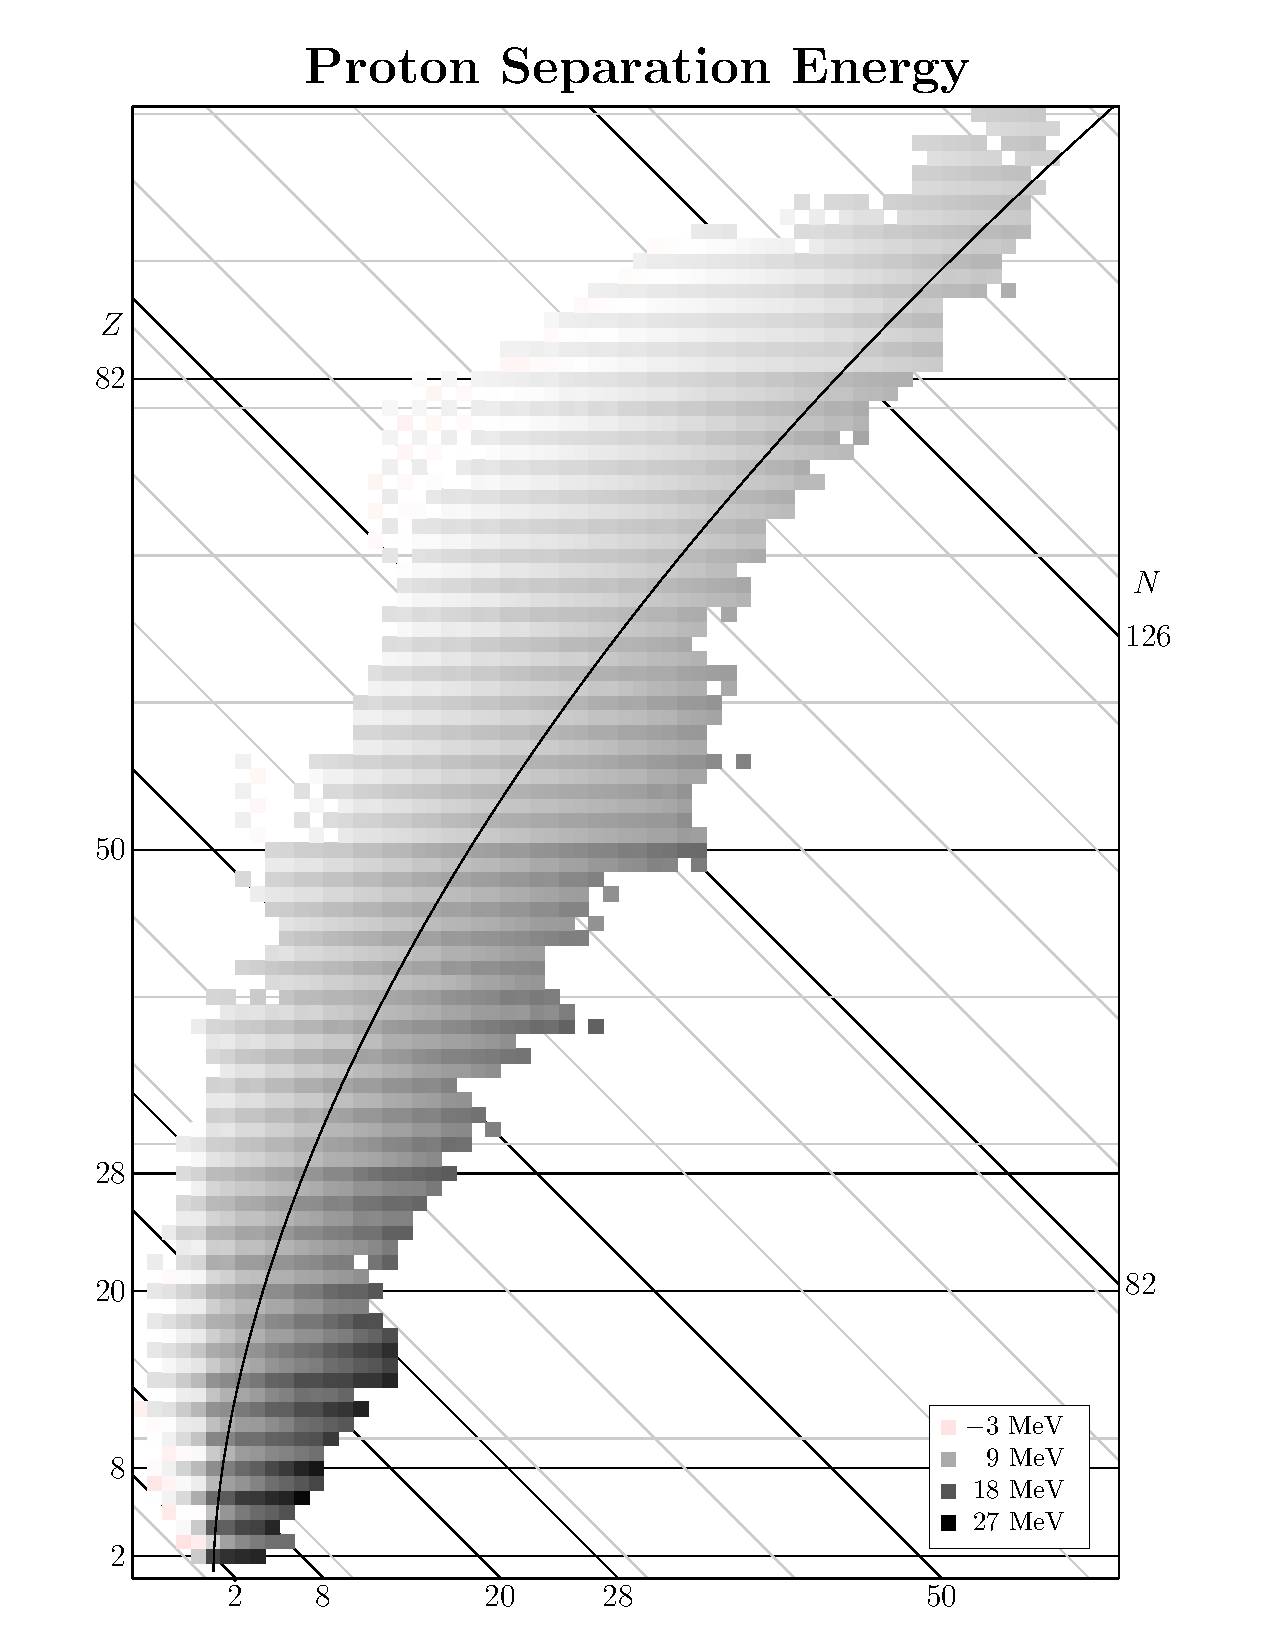
\includegraphics[width=0.35\textwidth]{figures/background/removal-energy.pdf}
	\caption{The amount of energy required to remove a proton from a nucleus as a function of Z and N~\cite{Dommelen}. This value, $E_i$, is used in the $x$-rescaling model.}
	\label{fig:nucleon-removal}
\end{wrapfigure}
In the case of $x$-rescaling, the EMC effect is explained by nuclear binding and Fermi motion corrections~\cite{GarciaCanal:1984eh, Staszel:1983qx}. In this case, the universal $x$-dependent behavior is explained by x having to be scaled up to a $x_A>x$. In the case of DIS, a nucleon $i$ with momentum $p_i$, the Bjorken-$x$ variable is replaced by:
\begin{equation}
x = \frac{Q^2}{2 p_i q} \rightarrow x_A = \frac{Q^2}{2(M+E_i)\nu - 2 \vec{p}_i \vec{q}}
\end{equation} 
where $\vec{q}$ is the momentum of the virtual photon and $E_i$ is the removal energy of the nucleon, which can vary between -9 and \unit[-27]{MeV}, depending on the nucleus and whether or not the nucleon in question is a proton or neutron (Fig.~\ref{fig:nucleon-removal}).

As a result of the $x$-rescaling, for the same scattered lepton in DIS, the momentum fraction $x_A$ is probed with regards to the structure function. Since the structure function falls off quickly with increasing $x$, the nuclear structure function ratio depletion is fully explained.

\section{The Role of Drell-Yan in Studying the Nuclear Quark Sea}

There have been many models attempting to explain the $A$-dependence of such phenomena as the EMC effect. Each of these models provides a prediction regarding the individual sea/valence quark/antiquark distribution functions. In order to test these predictions, one can take stock of the many nuclear probes and assess the capabilities of what each can contribute.

In general, since deep inelastic scattering of electrons and muons is an electromagnetic interaction, it is not innately sensitive to the whether or not the struck quark was a valence quark or a sea quark and can only measure the charge-weighted (E\&M+weak) sum of parton distributions. Through neutrino and antineutrino DIS it is possible to discern between valence and sea distributions. It is the case that most models make predictions for valence quark distributions at mid-to-high $x$ that are not in tension with each other. As such, measuring the valence distributions would not help much in discriminating between different models. Models do, however, differ in their predictions of the sea quark distributions at higher x ($x\gtrsim0.2$) - but at high momentum fraction, the distributions of sea quarks diminish very quickly (Fig.~\ref{fig:pdf-q2-q100}). As such, antineutrino DIS has been unable to deliver precise measurements of sea quark distributions at high-$x$ yet.

The Drell-Yan process, $pA\rightarrow l^+l^-$, uses the $s$-channel version of the same DIS process, but due to the nature of requiring interacting $q\bar{q}$ pairs, it provides a tool that allows one to cleanly and specifically investigate the sea quark distributions. With a forward spectrometer (such as is the case for E-772 and SeaQuest), where one accepts the $x_F>0.3$ one is able to study the Drell-Yan interaction in the specific case of a valence quark from a free proton (the beam) annihilating with an antiquark from the quark sea in the target. As a result, a study of this process for various nuclei can provide a direct, precise measurement of the antiquark sea distributions that can assist in evaluating the plethora of EMC effect models out there, along with refining constraints on global fits of PDFs.

In this paper, the A-dependence of the Drell-Yan cross sections is studied, which directly measures the A-dependence of the antiquark distributions~\cite{Berger:1985dr}. We define this ratio, $R^{DY}$ as the ratio of Drell-Yan differential cross-sections, using Eq.~\ref{eq:DY-cross} to get
\begin{eqnarray}
R^{DY} & \equiv & \frac{d^2\sigma_A}{dx_1 dx_2} \Biggm/ \frac{d^2\sigma_d}{dx_1 dx_2} \\
& \approx & \frac{\sum_f e_f^2 \cdot q_f^{\text{beam}}(x_1) \bar{q}_f^A(x_2)}{\sum_f e_f^2 \cdot q_f^{\text{beam}}(x_1) \bar{q}_f^d(x_2)}.
\end{eqnarray}
Assuming that the $\ubar$ distribution is roughly similar to the $\dbar$ distribution in the target, this term is dominated by up-quark contributions by a factor of eight: $e_u^2 = 4 e_d^2$, and there are twice as many up-quarks from the beam proton as down quarks~\cite{Geesaman:1995yd}. As a result, we can approximate
\begin{eqnarray}
R^{DY} & \approx & \frac{e_u^2 \cdot q_u^{\text{beam}}(x_1) \bar{q}^A_u(x_2)}{e_u^2 \cdot q_u^{\text{beam}}(x_1) \bar{q}^d_u(x_2)} \\ 
& = & \frac{\bar{q}_u^A(x_2)}{\bar{q}_u^d(x_2)}
\end{eqnarray}
meaning that by measuring $R^{DY}$ for $pA$ to $pd$ collisions with a forward spectrometer, a good measure of the nuclear modification of the anti up quark sea distributions can be achieved.

\subsection{Previous Measurements}

\begin{wrapfigure}{r}{0pt}
	\centering
	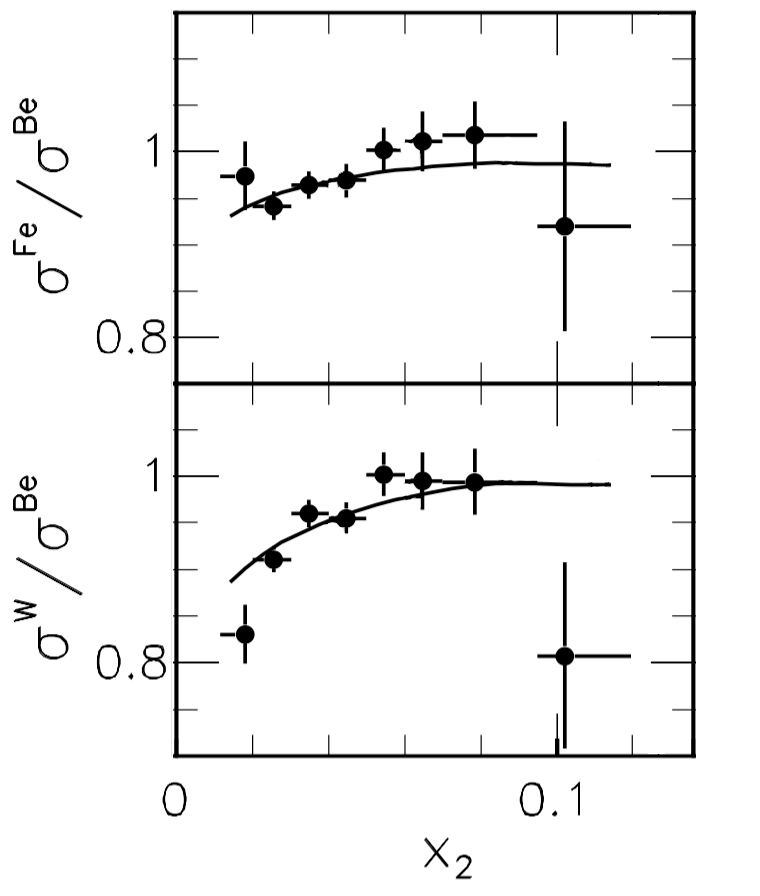
\includegraphics[width=0.35\textwidth]{figures/background/e866-emc-ratio.png}
	\caption{E-866 Drell-Yan $\sigma^A/\sigma^{Be}$ for iron and tungsten as a function of $x_2$~\cite{Vasilev:1999fa}.}
	\label{fig:866-emc}
\end{wrapfigure}
Even though Drell-Yan events for $x_F>0.3$ do directly provide a measure the sea quark distribution, there is a limited amount of data available. FNAL-E-772~\cite{PhysRevLett.64.2479} was a \unit[800]{GeV} fixed target experiment which provided a measure of $\sigma^A/\sigma^d$ for $C, Ca, Fe,$ and $W$ as a function of kinematic variable $x_2$. Soon to follow was FNAL-E-866~\cite{Vasilev:1999fa}, also a \unit[800]{GeV} proton beam fixed target experiment, which contributed a somewhat similar measurement of the DY cross section ratiof for $W$ and $Fe$ with respect to $Be$. The results which can be seen in Figures~\ref{fig:772-dy}~and~\ref{fig:866-emc} are able to show only a limited $x-$range of measurements of $0.05\leq x_2\leq 0.25$ for E-772 and $0.02\leq x_2 \leq 0.1$ (again, the sea quark distribution drops off sharply with increasing $x$). This data does show that at low-$x_2$ ($x_2 \lesssim 0.07$), there is indication of shadowing occurring. This makes sense for DY as well as DIS, even though there is no need the $\gamma\rightarrow q\bar{q}$ fluctuations, as the number of sea antiquarks increases greatly at this low range of $x$ and would thereby provide the same nucleon ``shadow'' as was described in Section~\ref{sec:shadowing}. 

For values above this shadowing region, the ratios appear to be consistent with unity. The range of $x$ covered line up with the \emph{transition region} (sometimes called ``anti-shadowing'') between the shadowing and EMC effect region. In some DIS measurements, this region can be characterized by having a value in excess of unity. A measurement of unity in the Drell-Yan cross section ratio would seem to imply that whatever this effect might be, it is likely not caused by any nuclear modifications to the sea quark distribution.

Regarding the other models, there was a great expectation that the Drell-Yan cross section would sizeably increase due to virtual pions which mediate the internuclear force. It was surprising that E-866 and E-772 observed no modification of the sea quark distributions in large nuclei, which brings into question the long-standing model of mesons being exchanged between nucleons as the mechanism by which nuclei are held together~\cite{Carlson:1997qn}.

To be able to truly draw any conclusions regarding various models, greater precision is needed, along with data at a higher-$x$ range where models are more greatly differentiated. The SeaQuest experiment will attempt to do just this.

\begin{figure}
	\centering
	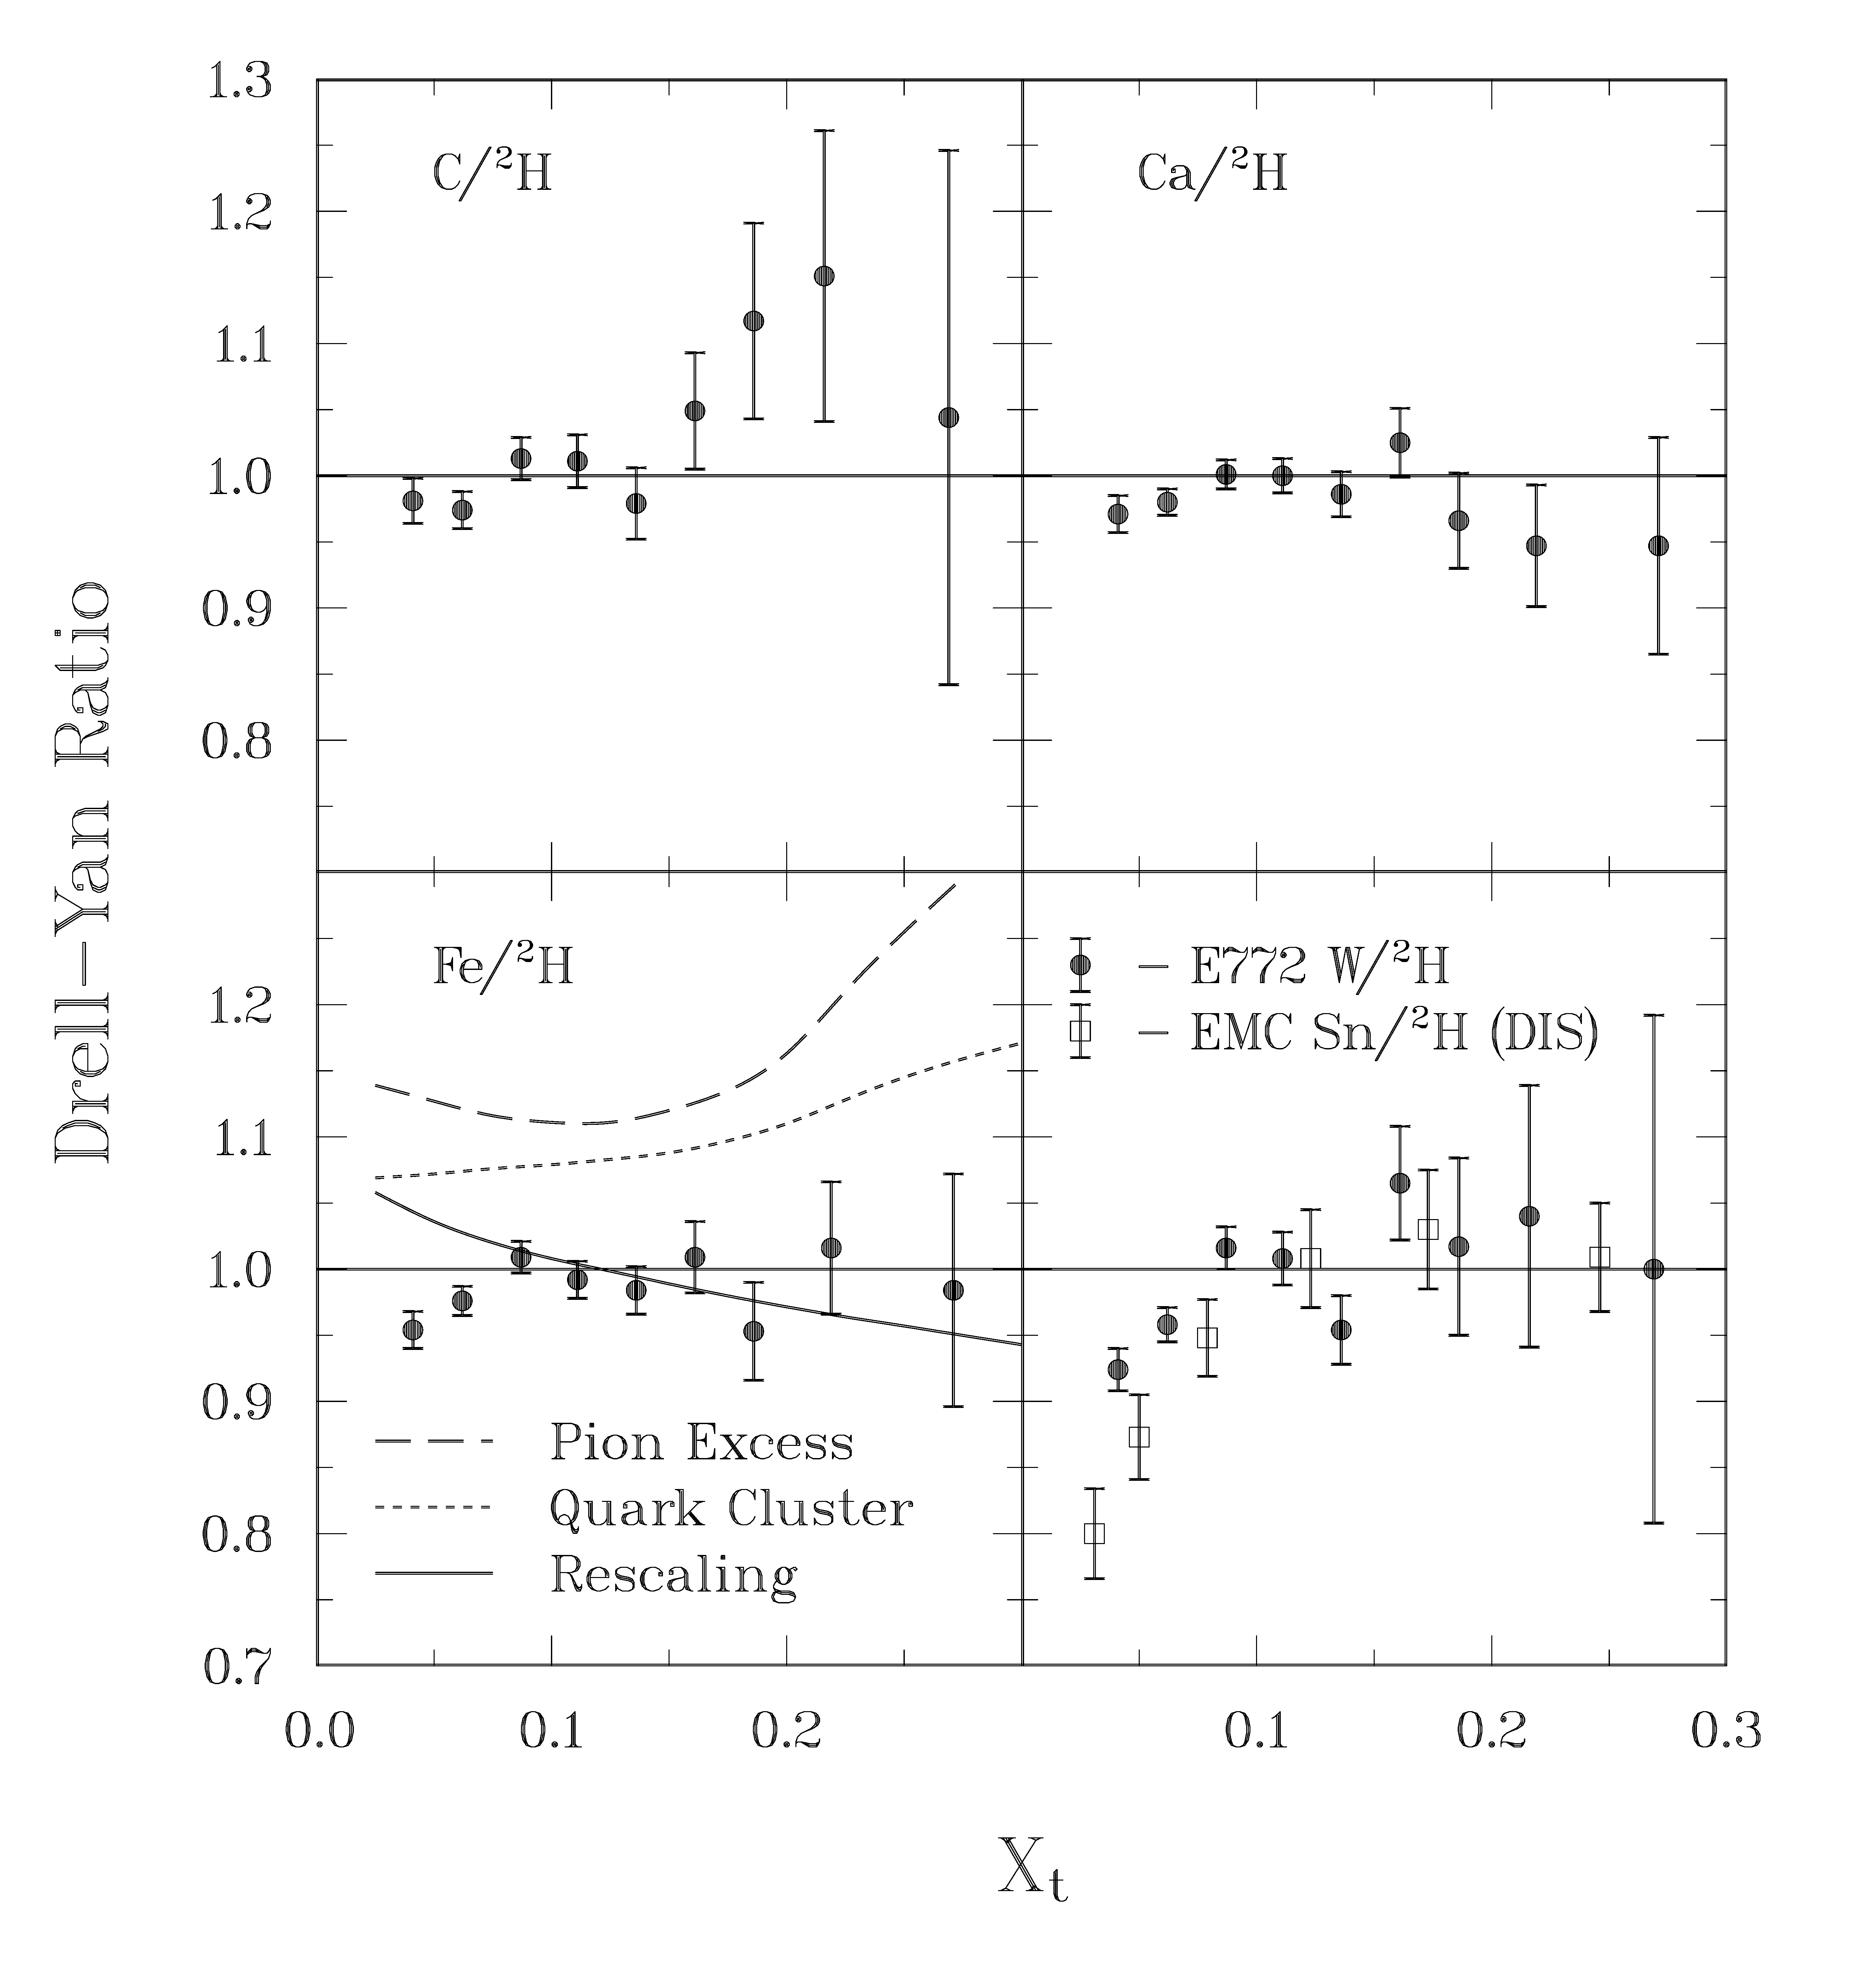
\includegraphics[width=\textwidth]{figures/background/dyfig9.png}
	\caption{E-772 Drell-Yan $\frac{A}{^2H}$ ratios for several nuclear targets as a function of $x_2$ ($x_t$)~\cite{PhysRevLett.64.2479}.}
	\label{fig:772-dy}
\end{figure}

\subsection{Nuclear Dependence of Drell-Yan at SeaQuest}

The SeaQuest Experiment was proposed soon after the conclusion of the E-866 experiment. The main motivation was to explore the $\dbar(x)/\ubar(x)$ value observed by E-866 to more precisely ascertain its behavior as a function of $x$. With the ratio value being as large as $\sim$1.7 at its peak and with it having a decreasing value at higher $x$ (though with low statistical certainty), no models are able to accommodate such behavior, and so more data is needed. 

Sea quark distributions at higher-$x$ the SeaQuest collaboration at Fermilab is designed to detect proton-induced Drell-Yan cross sections on several targets: liquid hydrogen ($^1H$), liquid deuterium ($^2H$), carbon ($^{12}C$), iron ($^{56}Fe$), and tungsten ($^{184}W$. The beam source for the experiment is the Fermilab Main Injector which provides a \unit[120]{GeV} proton source, yielding a $\sqrt{s}$ of \unit[15.1]{GeV}. This relatively lower beam energy as compared to \unit[800]{GeV} ($\sqrt{s}=\unit[38.8]{GeV}$) for E-772/E-886 provides an opportunity to study parton distributions at larger $x$. This is due to the fact that, as seen in Eq.~\ref{eq:DY-cross}, for a fixed value of $x$, the Drell-Yan cross section is inversely proportional to the square of the center-of-mass energy, $s$. Another benefit of utilizing a lower-energy beam is that the primary background, $\Jpsi$ production, which limited the instantaneous luminosity in E-866, scales with s, and is thereby reduced. This allows SeaQuest the usage of a more intense proton beam, which is very useful when it comes to measuring a rare nuclear process like Drell-Yan.

Even though the emphasis of SeaQuest is on the $\dbar/\ubar$ measurement, the periodic data taking on deuterium and the heavy nuclear targets will allow for a measurement of $R^{DY}\approx\ubar^A(x)/\ubar^D(x)$ for a large range of $A$ and $x$, providing a more thorough glimpse into the modification of sea quark PDFs in the presence of a nuclear medium. The general kinematic coverages and correlations for SeaQuest are shown in Figure~\ref{fig:x1-x2-acceptance}, as generated by Geant4 Monte Carlo simulation.

At the time of this writing, SeaQuest is the only fixed target proton-nucleon Drell-Yan experiment currently taking data in the world.

\begin{figure}
	\centering
	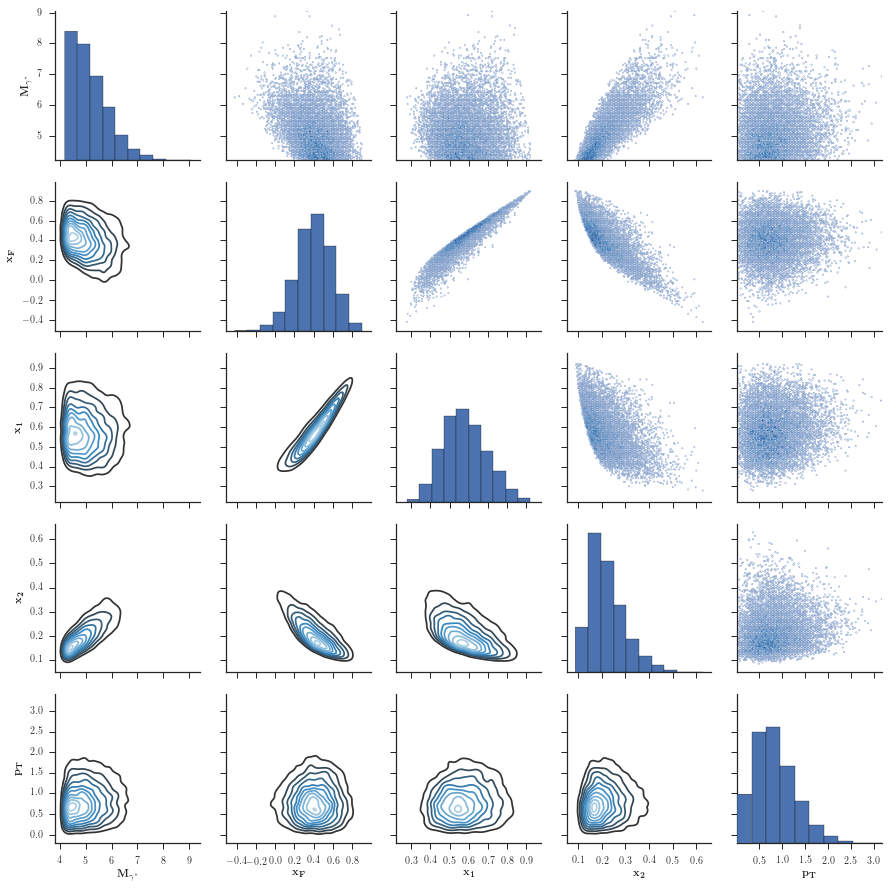
\includegraphics[width=\textwidth]{figures/background/pairplot-kin.png}
	\caption{A pairplot of the kinematic coverage of SeaQuest, based on weighted Geant4 Monte Carlo simulation, with $\unit[4.2]{GeV} < M_{\gamma^*} < \unit[10]{GeV}$ requirement imposed. The diagonal shows a histogram of the single kinematic, while the off-diagonal plots show the contours (bottom left) and scatterplots (top right) of the correlations between variables.}
	\label{fig:pairplot-kin}
\end{figure}
\chapter{Apparatus}

SeaQuest is the operational name of Fermilab Experiment \#906 (\emph{E-906}) performed at its Neutrino-Muon (\emph{NM})
experimental area. The experiment was designed
to take \emph{high-intensity beam} at relatively \emph{low center-of-mass energy}, provide
\emph{good mass resolution}, and allow for \emph{accurate target-to-target systematic normalization}.
The apparatus consists of a moving target table, two dipole magnets, 8 hodoscope planes, 24 drift 
chamber planes, and 4 proportional tube planes. Upstream of the target table (towards the beam source),
there is also a \v{C}erenkov counter for beam intensity monitoring and there are
several segmented wire ionization chambers (SWIC's) for beam profiling.

\section{Apparatus Overview}

SeaQuest is a fixed-target experiment. In this style of
experiment, a stationary target is placed in the path of an accelerated beam of particles, as opposed to \emph{collider} 
experiments where two accelerated beams are directed against each other, in opposite directions. The proton beam
interacts with the target material and produces a variety of daughter particles. These daughter particles are 
tracked through a forward spectrometer and selectively filtered dependent on the purpose of the study.

The tuned and monitored 120 GeV proton beam is sent from the Fermilab Main Injector (MI) where the beam
protons strike one of the 7 targets. The high-momentum charged particles that are produced are focused
onto the various detectors with the solid iron dipole magnet, FMAG, or NM3S. 
This solid focusing magnet also sweeps away low-momentum particles and acts as a beam dump / absorber.

\begin{figure}
	\begin{center}
		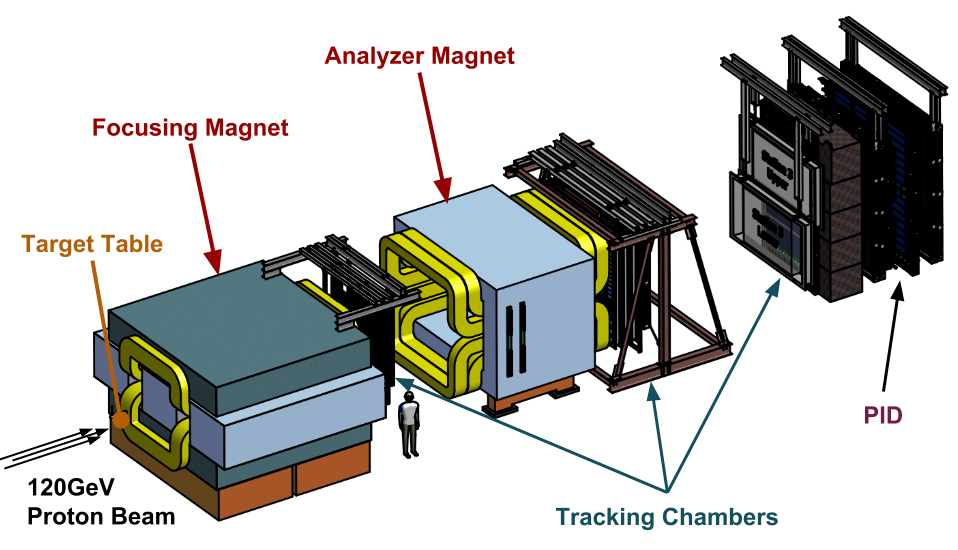
\includegraphics[width=0.75\textwidth]{figures/apparatus/Spectrometer.png}
		\caption{Perspective view of the SeaQuest spectrometer apparatus.}
		\label{fig:spectrometer-perspective}
	\end{center}
\end{figure}


The SeaQuest Spectrometer (Fig. \ref{fig:spectrometer-perspective}) consists of a focusing magnet to bend charged particles into the experiment's acceptance,
several tracking chambers that record the positions of charged particles through the length of the spectrometer, and
an analyzer magnet to bend the particles between tracking stations. The spectrometer measures particle momenta by
recording the bend of each charged particle as it passed through the analyzer magnet, where the magnetic field is known.
This is performed by reconstructing the trajectory of a particle in one-half of the spectrometer (before the
analyzer magnet) and then similarly reconstructing the trajectory of particles in the other half. If two 
trajectories can be matched up, then the particle momentum can be extracted by taking the ratio of the 
magnet's $p_T$-kick to the change in the track's direction.

The spectrometer geometric design and event
triggering selection is optimized to detect oppositely-charged pairs of muons while minimizing the sensitivity
to various sources of unwanted backgrounds. Positive identification of muons is achieved by requiring signals
in the hodoscopes for known muon \emph{``roads''} along with requiring signals in the proportional tubes located at
the farthest end of the experiment, past an iron wall. Electrons and any hadrons are stopped by the solid iron
focusing magnet an iron wall further down while muons will pass through them unencumbered.

The coordinate system is defined as the following: the \emph{z}-axis points along the beam direction, the
\emph{y}-axis points upwards vertically, and the \emph{x}-axis lies along the horizontal direction
in such a way that a right-handed coordinate system is formed. The terms \emph{upstream} and 
\emph{downstream} are often used when referring directions or regions in the experimental hall.
\emph{Upstream} often refers to the region of the experiment towards the beam source, while
\emph{downstream} refers to everything towards the $+z$ direction. 
The origin of the coordinate system was chosen to be the point where the proton beam meets 
the \emph{upstream}-facing surface of FMAG, the solid focusing magnet.


\section{Main Injector Proton Beam}

%% January 7th begin

The Fermilab Main Injector (MI) receives protons that have been accelerated by the Radio Frequency Quadrupoles (RFQ), 
the Linear Accelerator (LINAC), and the Booster, and it continues to accelerate them from 8 GeV up to the nominal energy
of 120 GeV. Along the way, the radio-frequency cavity (RFC) accelerators in the LINAC and the MI ``bunches'' up the
protons such that the beam has its characteristic 53.1 MHz structure. After the period of acceleration, the protons
are then 'scraped off' slowly with each passing \emph{turn} of the collected proton beam and sent down the
Neutrino-Muon (NM) beam delivery line for approximately five seconds of every minute, called a ``slow spill'', or just
``spill''. Beam is extracted using a resonant process, and the extracted beam retains the 53.1 MHz structure of the
Main Injector RFC. Each bunch, or ``bucket'', of protons is less than 2 ns long and the time between bunches is approximately
18.8ns. The spill structure of the beam is depicted in greater detail in Figure \ref{fig:SpillStructure}.

\begin{figure}
	\begin{center}
		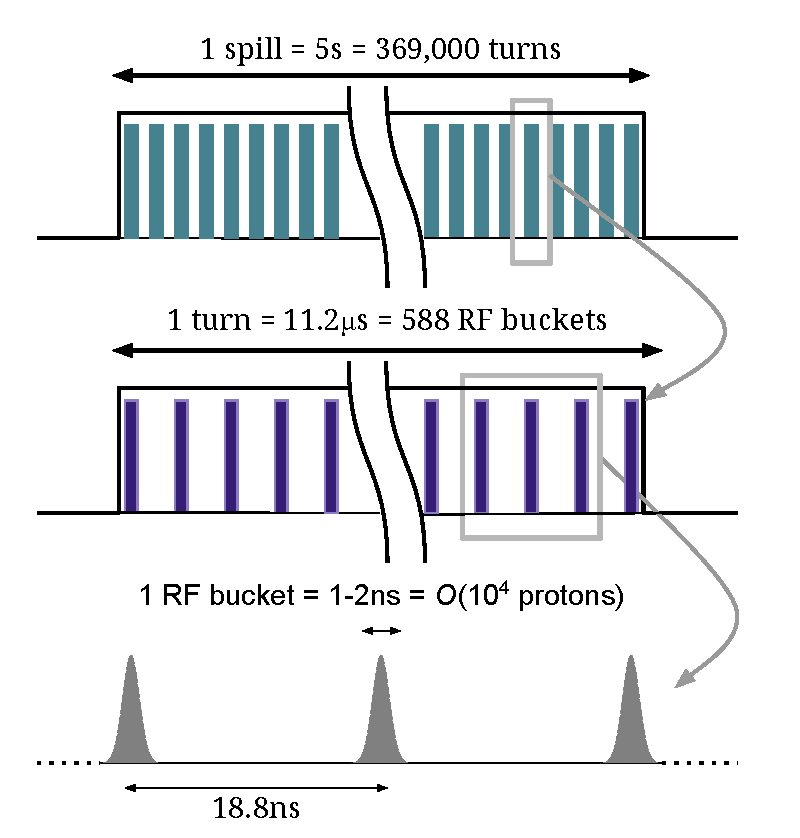
\includegraphics[width=0.55\textwidth]{figures/apparatus/SpillStructure.pdf}
		\caption{Spill structure of the beam delivered to SeaQuest.}
		\label{fig:SpillStructure}
	\end{center}
\end{figure}

The beam sent to SeaQuest is not uniform in time throughout the spill (in more ways than one).  There are beam bunches in the
MI that are intentionally left empty so that the abort kickers can ramp to a full field during a gap in the beam. There are also
bunches left empty to allow the injection kickers to inject 8 GeV protons from the Booster without disturbing bunches of protons
already in the Main Injector.  Typically, 498 of the 588 ``RF buckets'' in the Main Injector contain protons during the SeaQuest
slow spill cycle.  It is the case, however, for SeaQuest, that the intensity of the bunches corresponding to these 498 full
buckets varies greatly throughout the slow spill. On \emph{average}, each bucket will have \emph{O}($10^4$) protons and the spill
has an intensity of approximately $2\times 10^{12}$ protons per second and therefore about $1\times 10^{13}$ protons delivered per spill.

Several guiding and focusing magnets bend and deliver beam to the NM beamline which serves both the test beam facility and SeaQuest at NM4.
The beam is focused to a width of 250$\mu$m. The profile, position, and intensity are measured along the NM beamline by several detectors.
The intensity of the beam is monitored by an ion chamber (IC) and a secondary emission monitor (SEM) in the NM3 sector. The beam profile
and position are monitored by SWICs and beam-position monitors (BPMs), respectively. The Accelerator Control Network
(ACNET) display of the SWIC readout can be seen in Figure \ref{fig:Profile}. The closest BPMs and SWICs to the spectrometer were
located in NM2 enclosure. The beam profile does not maintain its 250$\mu$m shape and spreads slightly as it moves towards the
spectrometer. The final beam profile is measured by inspecting the upstream-facing side of the solid targets, and it was found
to be approximately 6mm wide by 1mm high.

\begin{figure}
	\begin{center}
		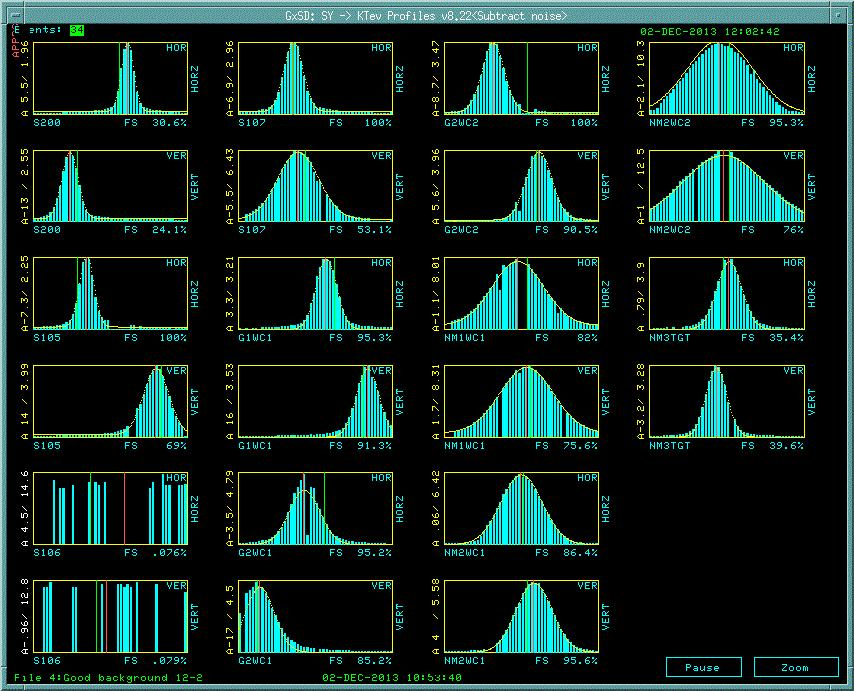
\includegraphics[width=0.65\textwidth]{figures/apparatus/swic.jpg}
		\caption{Beam profile detailed by SWIC detectors along the NM beam line.}
		\label{fig:Profile}
	\end{center}
\end{figure}

\section{Beam Intensity Monitor}

SeaQuest's trigger system (described in detail later) mostly fires on fake dimuons caused by two low $p_T$ muons from
unrelated pion decays. The hits in downstream hodoscopes from the pions combined with hits in the upstream
hodoscope from two other unrelated particles frequently add up to a false dimuon signal. Since this type of fake
trigger involves four unrelated particles, the probability that a trigger will occur increases with $I^4$, where
$I$ is the intensity of the beam bucket; the number of protons in the triggered beam bunch.

The SeaQuest data acquisition system (also described later in detail) can read out approximately 3000 events per
second without significant dead time.  During the commissioning run of SeaQuest, the trigger rate was very high and the
trigger dead time was close to 100\%.  These triggers were taken at such high beam intensities that the occupancy
of all SeaQuest detector elements was more than 50$\%$, making pattern recognition essentially impossible
(see Figure. \ref{fig:splat}). The Beam Intensity Monitor (BIM) was designed to solve this problem.

\begin{figure}
	\begin{center}
		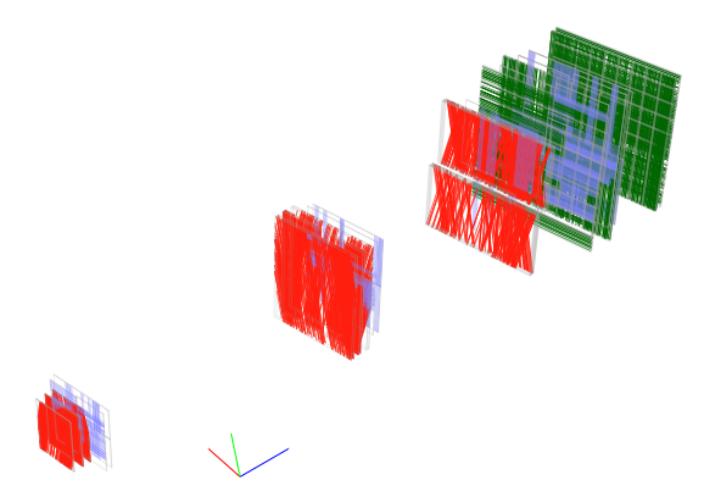
\includegraphics[width=0.5\textwidth]{figures/apparatus/splat2.png}
		\caption{A single high-intensity event with majority of all detector elements firing off. White space within the rectangles indicates inactive elements whereas red, blue, and green represent elements which have fired during that event. Track reconstruction in these cases is impossible.}
		\label{fig:splat}
	\end{center}
\end{figure}

The SeaQuest Beam Intensity Monitor (BIM) senses when the beam intensity is above a programmable threshold.
If an RF bucket with an intensity above this threshold is detected, the BIM sends a signal to inhibit
certain triggers until the intensity once more falls below the threshold. The inhibit threshold is tuned
frequently as trigger and beam conditions change, but the inhibit threshold is typically set at approximately
95,000 protons per RF bunch. For reference, a full RF bucket at an intensity of $2\times 10^{12}$ protons per
spill is $\approx$10,000 protons.

The beam intensity is measured using an atmospheric pressure gas \v{C}erenkov counter. A gas mixture of 80$\%$ Argon and 20$\%$ CO$_2$ is used as the \v{C}erenkov radiator. The counter and readout electronics were designed to have $O(ns)$ time resolution, and a linear response over a large dynamic range.  A diagram of the counter is shown in Figure~\ref{fig:BIMCerenkov}.  A 45 degree aluminized Kapton mirror directs light to a single photomultiplier tube.  A \emph{baffle} of black construction paper held parallel to the mirror ensures that the proton path length through the light-radiating gas with respect to the mirror is independent of beam position. A two-inch diameter 8-stage photomultiplier tube (PMT) is positioned close to the mirror so that all \v{C}erenkov light created between the baffle and the mirror falls directly on the aperture of the PMT. It was observed during the commissioning run
that after exposure to $\approx 3 \times 10^{17}$ protons (~3 weeks of uninterrupted usage), the mirror reflectivity is significantly reduced in the beam spot, and the mirror then needs to be replaced.

\begin{figure}
	\begin{center}
		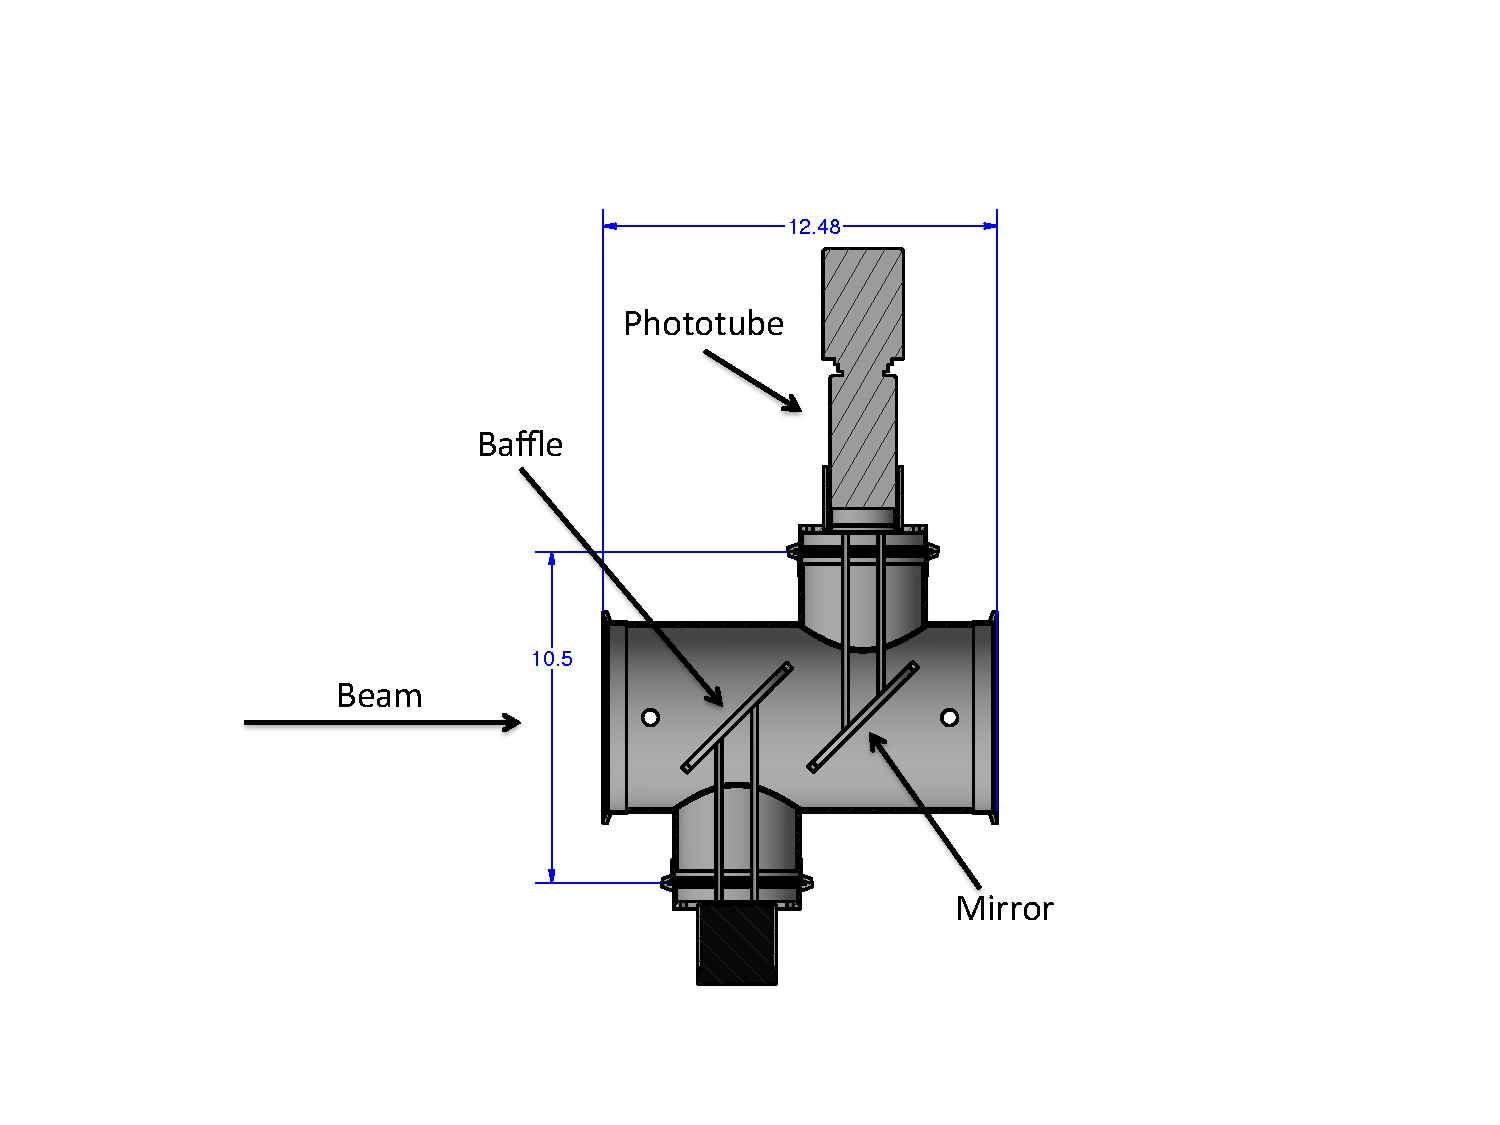
\includegraphics[width=0.6\textwidth]{figures/apparatus/BIMCerenkov.pdf}
		\caption{The Beam Intensity Monitor (BIM) \v{C}erenkov counter. Measurements are in inches.}
		\label{fig:BIMCerenkov}
	\end{center}
\end{figure}

The signal from the BIM is integrated and digitized using a custom charge (Q) integrator and encoder (\emph{QIE}) integrated circuit board, which comes from a family of circuits used first by the KTeV experiment at Fermilab\cite{QIE}. The chip is clocked with the Main Injector RF clock and provides an ADC (analog-digital conversion) every 18.8ns clock cycle. The light incident on
the photomultiplier tube is attenuated using neutral density filters (NDF's) so that the QIE least count corresponds to
$\sim$30 protons per beam bunch.

In addition to inhibiting triggers during high-intensity periods of beam, the BIM readout module also provides critical
information used to calculate the number of protons incident on the SeaQuest targets while the experiment is ready
and able to trigger. This value is needed to normalize SeaQuest cross section measurements. The BIM readout module provides the following:
\begin{itemize}
	\item Sum of all ADC signals for the entire spill (QIESum).
	\item Sum while inhibit is asserted at trigger logic.
	\item Sum during trigger dead time.
	\item A snapshot of beam intensity 16 buckets before and after the triggered RF bucket
\end{itemize}

These are used to calculate a ratio of protons that were `live' (the experiment can trigger) via the following:
\begin{eqnarray}
liveRatio & = & \frac{QIESum - (inhibit\ sum + dead\ time\ sum)}{QIESum} \\
liveProton & = & totalProton \cdot liveRatio
\label{eqn:liveproton}
\end{eqnarray}
where ``totalProton'' is the intensity value recorded from the SEM detector located just upstream of the BIM \v{C}erenkov counter. The SEM itself is calibrated by foil activation. The snapshot of the triggered RF bucket intensity along with the 32 surrounding RF bucket intensities is used for studies and corrections of the rate-dependent effects on detector efficiencies and reconstructed measurements.

\section{The SeaQuest Targets}

\begin{table}[p]
	\begin{center}
		\begin{tabular}{c c c c c c c}
			\parbox{1.5cm}{\centering{~\\Position} } & \parbox{1.5cm}{\centering{~\\Material} }  &\parbox{1.5cm}{\centering{Density\\{[g/cm$^3$]}} }  &  \parbox{1.75cm}{\centering{Thickness\\{[cm]}} }& \parbox{2cm}{\centering{Interaction\\Length} }&  \parbox{1.5cm}{\centering{Spills/\\Cycle\\(\%spills)} } \\ [0.5ex] \hline
			1 & $H_2$     & 0.07065 & 50.8  & 0.06902 & 10 (43\%) & \\
			2 & Empty     & NA      & NA    & 0.0016  & 2 (9\%)  & \\
			3 & $D_2$     & 0.1617  & 50.8  & 0.1144  & 5 (22\%)  & \\
			4 & None      & NA      & NA    & 0.0     & 2 (9\%)  & \\
			5 & Iron      & 7.874   & 1.905 & 0.1135  & 1 (4\%)  & \\
			6 & Carbon    & 1.802   & 3.322 & 0.0697  & 2 (9\%)  & \\
			7 & Tungsten  & 19.30   & 0.953 & 0.0958  & 1 (4\%)  & \\ [0.5ex] \hline
		\end{tabular}
		\caption{Characteristics of the seven SeaQuest target positions.  The ``Spills/Cycle'' is only a typical configuration and can vary according to needs and running configurations.  The non-zero interaction length of the empty flask is due to the 51$\mu$m-thick stainless steel end-caps of the flask and the 140 $\mu$m-thick titanium windows of the vacuum vessel that contains it.}
		\label{tab:target-materials}
		
	\end{center}
\end{table}

\begin{figure}[p]
	\begin{center}
		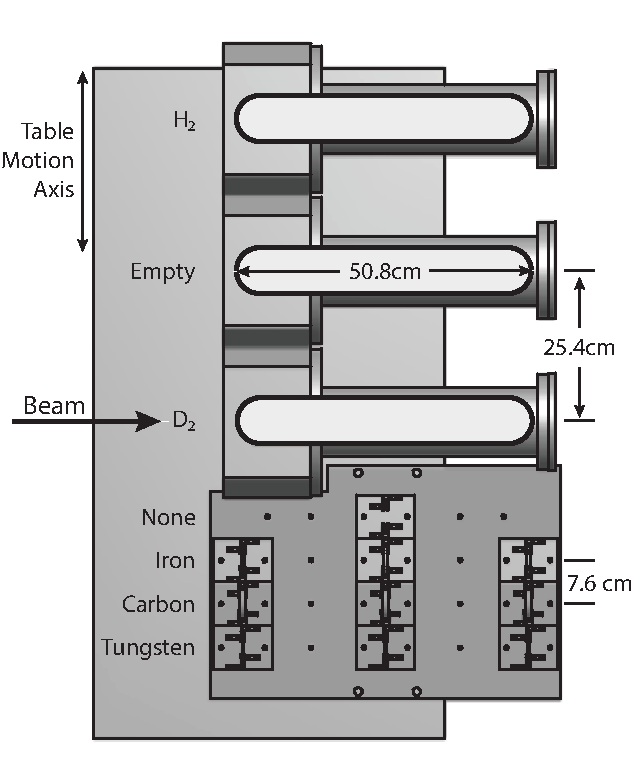
\includegraphics[width=0.65\textwidth]{figures/apparatus/target-tableLayout.pdf}
		\caption{The layout of the target table and its seven target positions, as seen from above.}
		\label{fig:table-layout}
	\end{center}
\end{figure}


A wide range of atomic weights (from 2 to 184) is required to do an A-dependence study of the Drell-Yan process.
At SeaQuest, the targets used are $^1H (\ell),\ ^2H (\ell),\ C,\ Fe,\ $and$\ W$. In addition to the two liquid targets
and the three solid targets, two positions on the target table were used for measuring background signal rates:
an empty flask, identical to the flasks used for the $^1H$ and $^2H$ targets, and a single empty solid target holder.
Colloquially speaking: the $^1H$ target is interchangeably referred to as the liquid hydrogen target, $\ell H_2$,
\emph{LH2}, or $H_2$; $^2H$ is likewise referred to as the liquid deuterium target, $\ell D_2$, \emph{LD2}, or $D_2$;
the empty flask is referred to as the ``Empty'' target; the empty solid target holder is referred to as the ``None'' target.

These are all mounted on a laterally-moving, remotely positionable table (in the $\pm x$ direction), able to move
over a range of 91.4cm. The table's center is located at $(0, 0, -1.25)$ meters, directly in front of the upstream face
of FMAG, the solid iron focusing magnet. Because of the $\sim$5.0cm diameter of the targets and the 6x1mm dimensions of the beam, the targeting efficiency was 100\%. The details of the target materials are summarized in Table \ref{tab:target-materials}, and the layout of the target table can be seen in \ref{fig:table-layout}.

The $H_2$ gas used is ``Ultra High Purity 5.0 Grade'' or 99.999\% pure.  The deuterium has come from two different
sources.  The first of these is a Fermilab-provided supply of gas left over from previous bubble chamber experiments.
This gas was known to have a small hydrogen contamination and was measured by mass spectroscopy to have a composition
of 85.2\% D$_2$, 12.7\% HD, 1.2\% $^4$He, and 0.8\% H$_2$ by mole. As the analysis of experimental data commenced, 
handling the ramifications of the D$_2$ impurity came under focus. Unexpected bottle-to-bottle variation in contamination
became evident, and the sample-taking methodology itself for spectroscopy became suspect of introducing contamination.
In order to no simplify analysis and reduce the substantial complexity and cost of further gas analysis, SeaQuest switched
to commercially available ``Research Grade'' D$_2$, which is better than 99.6\% pure with virtually all HD to balance.
The data analyzed in this paper deals with the impure D$_2$ target material before this switch. Further information on
the D$_2$ composition and how it is handled in the context of analysis will be covered in Chapter 4.

%10'' apart to approximate the 20'' 
%  more closely spaced (6.73'').

Each of the three solid target positions is divided into three disks of 1/3 the total thickness provided in Table \ref{tab:target-materials}. These disks are spaced 25.4cm apart to approximate the distribution of the liquid target, thereby minimizing target-dependent variation in spectrometer acceptance. The one exception to this is that during the Run II period the iron plugs were more closely spaced (17.1cm). The decision to place these
iron disks closer together than the rest during Run II is still unclear.

The target table is able to move between two different targets in about 30 seconds. This allows a change between targets in the 55 seconds between successive spills. With this frequent target interchange, the systematic uncertainties associated with drifts in beam characteristics, monitor gains, and detector efficiencies are reduced to a minimum when investigating A-dependent ratios. How much beam time each target received is determined by interaction lengths of the targets along with the amount of statistics desired for certain targets. As the flagship measurement of SeaQuest is the $\bar{d}/\bar{u}$ asymmetry, more emphasis was placed on the hydrogen and deuterium than the nuclear targets. The spills per cycle and beam time allocation can be found in Table \ref{tab:target-materials}.

\section{Focusing and Analyzing Magnets}

Two large dipole magnets are used in the experiment to be select forward going ($x_F > 0$) dimuons, reject low-momentum particles, and analyze their kinematic characteristics. The most upstream magnet, denoted ``FMAG'', is a solid iron A-frame magnet with an aperture of 1.22m in the $x$-direction and 66cm in the $y$-direction. It is assembled from 43.2cm x 160cm x 503cm iron slabs, as shown in Fig.~\ref{fig:FMag}. The magnet has no air gap, and the iron has extremely high purity, allowing a 2000A excitation current to generate a nearly constant, central magnetic field of 1.9 Tesla (yielding a 2.91 GeV/c total magnetic deflection). The field is generated by exciting the embedded aluminum \emph{``bedstead''} coil to 2000 Amps at 25 Volts (50 kW).  The current exciting FMAG is monitored by the Fermilab ACNET system and is broadcast to the SeaQuest slow data acquisition system every acceleration cycle. The excitation is also input to the beam-disabling safety system in order to prevent the beam from hitting the SeaQuest spectrometer when FMAG is not fully powered. FMAG also acts as the beam dump for the 120 GeV beam. There is a 5cm diameter by 25cm deep bore drilled into the upstream end of FMAG (recall, this is the origin of the experiment's coordinate system).  The 120 GeV protons that do not interact in the SeaQuest targets 125cm upstream of FMag, interact in the central iron slab.  Most of the 2.0 kW beam power is dissipated in this slab and is eventually conducted to the coils and external surfaces to be radiated away.

\begin{figure}
	\centering
	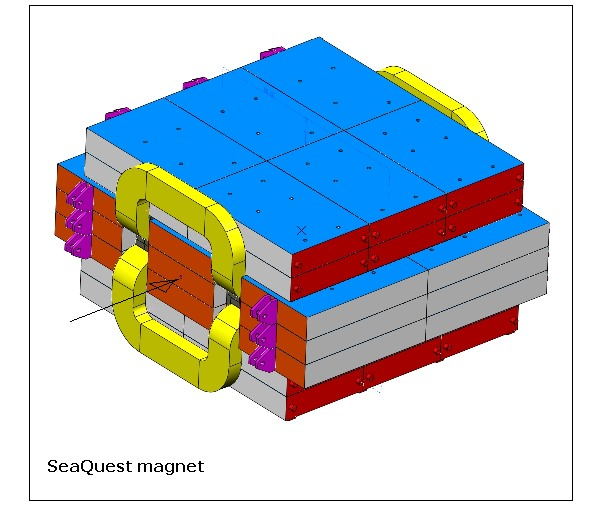
\includegraphics[width=8cm]{figures/apparatus/FMAG}
	\caption{Perspective drawing of FMAG's aluminum coils embedded in an arrangement of iron slabs.}
	\label{fig:FMag}
\end{figure}

The downstream magnet, denoted ``KMAG'', is a 300cm long iron rectangular magnet with a 289cm wide by 203cm high central air gap.  It was originally constructed by the KTeV collaboration~\cite{PhysRevD.67.012005} at Fermilab.  It is excited to a central field of 0.4 Tesla (0.402 GeV/c magnetic deflection) by 1600 Amps at 270 Volts (430kW).  The spatial distribution of the magnetic field in KMAG was measured by the KTeV group and re-verified by SeaQuest.  In normal running conditions, both FMag and KMAG bend muons horizontally in the same direction. This two-magnet configuration is often referred to as a focusing spectrometer.

The 2.91 GeV/c and 0.402 GeV/c magnetic deflections deliver a transverse-momentum ($p_T$) kick along the to charged particles passing through the spectrometer. The magnets bend the paths of the muon in the $\pm x$ direction, with the sign depending on the orientation of the magnetic fields and the particles' charges. Between Run II and Run III of data taking, the current direction was reversed, thereby reversing the direction of the magnetic fields. During Run II, the magnetic fields were pointing in the $-y$ direction, and in Run III, the magnetic fields were flipped to point in the $+y$ direction. This was done for two reasons: (1) to identify any left-right asymmetries in the experiment, and (2) to limit the amount of radiation on the electronics in the experimental hall, as a large number of positive particles were being swept directly towards the electronics racks during Run II.

\section{Beam Dump, Shields, and Absorbers}

In order to prevent damage to the downstream detectors from the beam and reduce signals from incidental radiation, the spectrometer is designed with a beam dump and two hadron absorber walls. Approximately 125cm downstream of the target table
is the water-cooled beam dump whose upstream face is located at $(0.0, 0.0, 0.0)$ m. The beam dump is one of the many solid iron 5m blocks that fill and surround the FMAG coils. The whole length of the beam dump along the beam axis is equivalent to $\approx 35$ nuclear interaction lengths of iron. 

Between the downstream face of FMAG and Station 1, there is a 2 cm thick wall of borated polyethylene which is put in place as a fast neutron shield. This material is 5\% boron by weight, with the rest being polyethylene. The polyethylene contains high hydrogen content, making it an effective fast neutron radiation shield, slowing down the fast neutrons down to thermal speeds. The boron in the material provides attenuation of thermal neutrons, thus reducing the levels of capture-gamma radiation elsewhere in the experiment. Borated polyethylene at this thickness is a common and optimal neutron shielding material for areas of low to intermediate neutron flux where the temperature is below $82^\circ$C \CN. These conditions make the downstream side of FMAG ideal for its placement.

Farther downstream, there is another hadron absorber wall located between Station 3 and Station 4. The absorber wall consists of a stack of 98cm thick iron blocks. This is an equivalent of $\approx 6$ nuclear interaction lengths. The purpose of this wall is to identify muons at the rear of the apparatus by effectively blocking all other types of particles. The only charged particles which can penetrate this absorber wall are muons.

\section{Tracking Detectors}

The tracking detectors are the instruments used for measuring the values of the kinematic variables of the dimuon pairs. Several different types of detectors are grouped together to form a detector \emph{Station}. The types of detectors used are hodoscopes, wire chambers, and proportional tubes. There are four stations throughout the experimental hall that provide tracking information at different points along the spectrometer, numbered from 1 to 4 in order of increasing $z$. Station 1 is located between FMAG and KMAG. Station 2 is located at the downstream face of KMAG. Station 3 and 4 are just upstream and downstream, respectively, of the iron absorber wall. The Station layout can be seen in Fig. \ref{fig:stations}

\begin{figure}
	\centering
	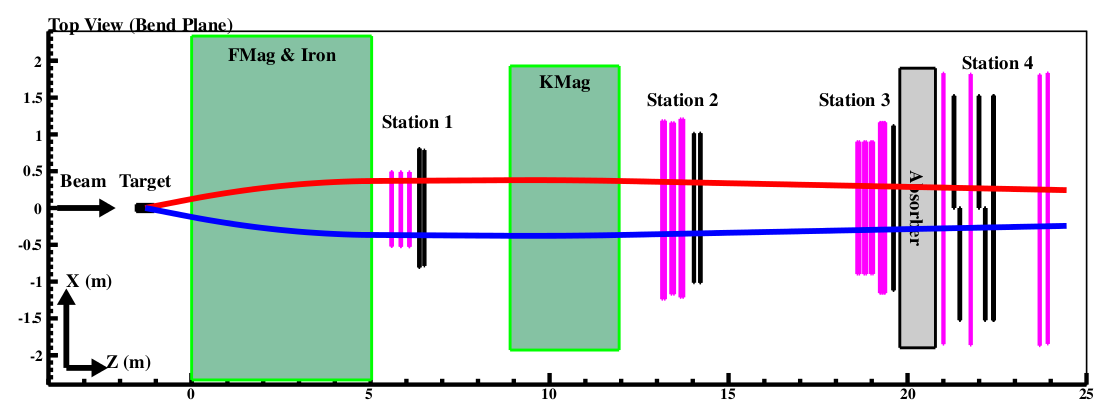
\includegraphics[width=0.75\textwidth]{figures/apparatus/stations.png}
	\caption{Spectrometer layout of FMAG, KMAG, and Detector Stations 1-4.}
	\label{fig:stations}
\end{figure}

\subsection{Triggering Hodoscopes}

Hodoscope arrays are located at each of the four detector stations. These detectors' primary usage is to select events with two opposite-signed muon tracks in them. Certain `roads' through the spectrometer are defined in the fast trigger logic, and when two desired roads are observed in a given event, the trigger system tells the data acquisition systems to record that event's data. In addition to this, the hodoscopes provide analysts with the ability to discard or ignore certain hits in adjacent chambers for which there is no corresponding nearby hodoscope hit. This is useful in decreasing the hit multiplicities in the wire chambers, which in turn decreases the combinatoric complexity of reconstruction algorithms.

Each of the eight hodoscope planes is split into two halves: top and bottom in the case of planes with vertically-oriented paddles, or left and right for planes with horizontally-oriented paddles (denoted by `T', `B', `L', and `R', respectively). In each half-plane, the hodoscopes are a set of long rectangles arranged `picket fence'-style with a small 0.3175cm overlap, as to prevent any particles from possibly slipping between paddles. A single hodoscope detector element is composed of plastic scintillator material connected to Philips XP 2008 photomultiplier tubes (PMT) by plexiglass light guides. Stations 1, 2, and 4 each have two hodoscope planes, with planes of both vertically- and horizontally-oriented paddles (for measuring in $x$ and $y$, respectively). Station 3 consists only of vertically-oriented plane, and thus measures in the $x-$direction only, which is in the experiment's $x-z$ bend plane. The hodoscope planes are named according to detector station and the direction that they measure. For example, the $y$-measuring hodoscope plane in Station 2 is called ``H2Y''. The individual half-planes are named according to detector station and which half it is of the two. For example, the top half of the $x$-measuring hodoscope plane in Station 1 is referred to as ``H1T''. As such, the ``H3X'' detector is composed of ``H3T'' and ``H3B''. The detailed specifications of each hodoscope plane are given in Table \ref{tab:hodoscopes}. A precise alignment of the hodoscopes was achieved by examining the distributions of positions of tracked muons at each hodoscope plane when a given hodoscope element in that plane was fired.

\begin{table}[bthp]\centering
	\begin{tabular}{llllll}
		\hline
		\hline
		Detector & Paddle & Overlap & \# of paddles & Width $\times$ Height & $z$-position [cm] \\
		& Width & [cm] & (per half-plane) & (per half-plane) &  \\
		& [cm] & & & [cm] $\times$ [cm] & \\
		\hline
		H1X & 7.32 & 0.3175 & 23 & 162 $\times$ 70 & 666 \\
		H1Y & 7.32 & 0.3175 & 20 & 79 $\times$ 140 & 653 \\
		H2X & 13.00 & 0.3175 & 16 & 203 $\times$ 152 & 1421 \\
		H2Y & 13.00 & 0.3175 & 19  & 132 $\times$ 241 & 1400 (L), 1406 (R) \\
		H3X & 14.59 & 0.3175 & 16  & 228 $\times$ 168 & 1959 \\
		H4X & 19.65 & 0.3175 & 16  &  305 $\times$ 183 & 2234 (T), 2251 (B) \\
		H4Y1 & 23.48 & 0.3175 & 16  & 152 $\times$ 366 & 2130 (L), 2146 (R) \\
		H4Y2 & 23.48 & 0.3175 & 16  & 152 $\times$ 366 & 2200 (L), 2217 (R)\\
		\hline
		\hline
	\end{tabular}
	\caption{Parameters of all hodoscope planes. $z$-positions of H2Y and H4 half-planes are offset slightly due to the half-planes themselves overlapping.}
	\label{tab:hodoscopes}
\end{table}

\subsection{Drift Chambers}

Each of Stations 1, 2 and 3 is equipped with a drift chamber (DC) to measure the passing $x$ and $y$ positions of muons at its $z$ location, with each DC flat vertical to the $z$ axis, and a drift cell is of the box shape. These measured positions are critical for reconstructing the trajectory of muons, and thereby their kinematics. Each DC contains six drift chamber planes, arranged in three pairs with parallel wire orientations (each pair referred to as a ``view''). Wires oriented vertically ($x$-measuring) are referred to as being in the ``X'' view and at angles of $+14^\circ$ and $-14^\circ$ with respect to the $y$-axis are the ``V'' and ``U'' planes, respectively. The second plane in each view is offset from the first by one-half of a wire-to-wire distance (\emph{``cell width''}) in order to resolve the left-right ambiguity of drift direction. This offset plane of each pair is referred to as the \emph{primed} plane, and is denoted with a `$\prime$'. So, in each DC, there are X, X$^\prime$, U, U$^\prime$, V, and V$^\prime$ planes, with primed and unprimed planes (like X and X$^\prime$) constituting a view.

The individual drift chambers at Stations 1 and 2 are called ``D1'' and ``D2'', respectively. Station 3 has two drift chambers since the desired acceptance area it has to cover is substantially larger than one DC can cover. These are split vertically to cover the top and bottom halves, and are called ``D3p'' and ``D3m'' where ``p'' and ``m'' stand for ``plus'' and ``minus''. Table~\ref{table:cham:param} summarizes the parameters of the DC's. D1 and D3m have been upgraded during the data taking, as listed in Tab.~\ref{tab:cham:comb1}. This original and upgraded versions are referred to as D$N$.1 and D$N$.2, respectively.

\begin{table}[bthp]\centering
	\begin{tabular}{cc|cccc}
		\hline \hline
		Chamber & Plane & Number   & Cell  & Width            & $z$-position \\
		&       & of wires & width & $\times$ height  &      \\ 
		&       &          & [cm]  & [cm] $\times$ [cm] & [cm] \\ 
		\hline
		D1.1    & X     & 160      & 0.64  & 102 $\times$ 122 &  617    \\
		& U, V  & 201      & 0.64  & 101 $\times$ 122 & $\pm$20 \\
		D1.2    & X     & 320      & 0.50  & 153 $\times$ 137 &  617    \\
		& U, V  & 384      & 0.50  & 153 $\times$ 137 & $\pm$1.2 \\
		D2      & X     & 112      & 2.1   & 233 $\times$ 264 & 1347    \\
		& U, V  & 128      & 2.0   & 233 $\times$ 264 & $\pm$25 \\
		D3p     & X     & 116      & 2.0   & 232 $\times$ 166 & 1931    \\
		& U, V  & 134      & 2.0   & 268 $\times$ 166 & $\pm$6  \\
		D3m.1   & X     & 176      & 1.0   & 179 $\times$ 168 & 1879    \\
		& U, V  & 208      & 1.0   & 171 $\times$ 163 & $\pm$19 \\
		D3m.2   & X     & 116      & 2.0   & 232 $\times$ 166 & 1895    \\
		& U, V  & 134      & 2.0   & 268 $\times$ 166 & $\pm$6  \\
		\hline
		\hline
	\end{tabular}
	\caption{Parameters of all chambers.
		Those of primed planes are almost the same as of unprimed planes.
		The $z$-positions of U and V planes are relative to those of X planes.
	}
	\label{table:cham:param}
\end{table}

\begin{table}[bthp]\centering
	\begin{tabular}{ccc}
		\hline
		Run & Period & Chamber combination \\
		\hline
		1 & 2012 Mar.-2012 Apr.  &  D1.1, D3m.1 \\
		2 & 2013 Nov.-2014 Aug.  &  D1.1, D3m.2 \\
		3 & 2014 Nov.-2015 May   &  D1.1, D3m.2 \\
		3 & 2015 Jun.-2015 Jul.  &  D1.2, D3m.2 \\
		4 & 2015 Sep.-   &  D1.2, D3m.2 \\
		\hline
	\end{tabular}
	\caption{Combination of D1 and D3m chambers per data taking period.}
	\label{tab:cham:comb1}
\end{table}

The acceptance size of each chamber has been adjusted with a Drell-Yan event simulation in order to be as sensitive as possible to the $x_2$ range of interest. Particularly, the greater the acceptance width is, the higher the reach in $x_2$ is. This makes the hit-rate tolerance of the chambers a key feature because the spectrometer is exposed to a large number of background particles, particularly near the edges where the desired $x_2$ events occur. It is particularly significant for the most-upstream station (i.e.~Station 1) which receives the highest hit rates. Experimental data shows that the rate tolerances are 3.0 MHz/wire at D1, 1.6 MHz/wire at D2 and 0.7 MHz/wire at D3 with a beam intensity of $5\times 10^{12}$ protons/spill. The gas-amplification gain should not be degraded under these hit rates.

For Run 2 and beyond, the gas mixture used for almost all the chambers is Argon:Methane:CF4 (88\%:8\%:4\%) with a drift velocity of about 20 $\mu$m/ns. A ``fast gas'' mixture used for D1.2 (upgraded D1) is Argon:CF4:Isobutane:Methylal (68\%:16\%:13\%:3\%) with a drift velocity of 50 $\mu$m/ns and thereby a better hit-rate tolerance. This is ``fast'' in comparison to the $\approx 20\mu$m/ns rest of the DCs. The spatial resolution of each plane is required to be 400$\mu$m, which corresponds to a momentum resolution of $\Delta p / p = 0.03 \cdot p$ (GeV/$c$). The resolution of dimuon invariant mass is dominated by the multiple scattering in FMAG; the chamber momentum resolution is about 10\% of the total mass resolution at maximum.

The D1.1, D2, and D3m.1 chambers have been inherited from previous Drell-Yan experiments that have been conducted at Fermilab.
Chambers D2 and D3m.1 have their origin in E-906~\cite{PhysRevD.43.2815} and D1.1 is from SeaQuest's direct predecessor, E-866/NuSea~\cite{PhysRevLett.80.3715, Towell:2001nh}. Since these chambers have not been used for decades since E-866, they had to be refurbished by restringing $\approx 30\%$ of their sense wires due to them being loose or broken. Newly supplied electronic readout boards were also mounted on these chambers.

The D3p and D3m.2 chambers were designed and constructed specifically for this experiment in order to cover the large acceptance required at Station 3. D3p was newly constructed by the TokyoTech SeaQuest collaborators and was shipped from Japan to Fermilab. The first part of data taking, Run 1, was carried out using D3m.1 while preparing for the construction of D3m.2. The newer D3m.2 is wider than D3m.1 by 25 cm at each side, allowing the high-$x_2$ statistics on $\bar{d}/\bar{u}$ and $Y_A / Y_{^2H}$ to increase by $\approx 20\%$ at $x_2 \sim 0.3$ and $\approx 10\%$ at $x_2 \sim 0.4$. The operational stability also improved, as D3m.1 suffered from frequent dead/noisy wires, HV trips, and leak currents. The D1.2 chamber was also designed and constructed for this experiment by the University of Colorado Boulder. As it is wider than D1.1 by 25 cm at each side and greater hit-rate tolerance, the anticipated statistics is expected in the high-$x_2$ region is expected to increase still more. It was installed in the experimental hall near the end of Run 3.

\subsection{Proportional Tubes}

Downstream of Station 3 and the 1 m thick iron hadron absorber wall is Station 4 with its hodoscope planes and proportional tube  detectors (prop tubes). At Station 4, the only beam-induced particles that remain that can leave tracks in an ionization detector are high energy muons. The prop tubes enable the task of muon particle identification (PID) for the experiment and consist of four planes. Each detector plane is made of 9 prop-tube modules, with each module assembled from 16 12-ft long 2" diameter prop-tubes staggered to form two sub-layers. The first and fourth planes are oriented along the horizontal direction (tubes parallel to the floor) to provide positional measurements in $y$, as shown in Fig.~\ref{fig:proptube:xzview}. The second and third planes are arranged vertically to measure $x$-position as shown in and Fig.~\ref{fig:proptube:yzview}.

\begin{figure}
	\centering
	\begin{minipage}[t]{0.49\linewidth}
		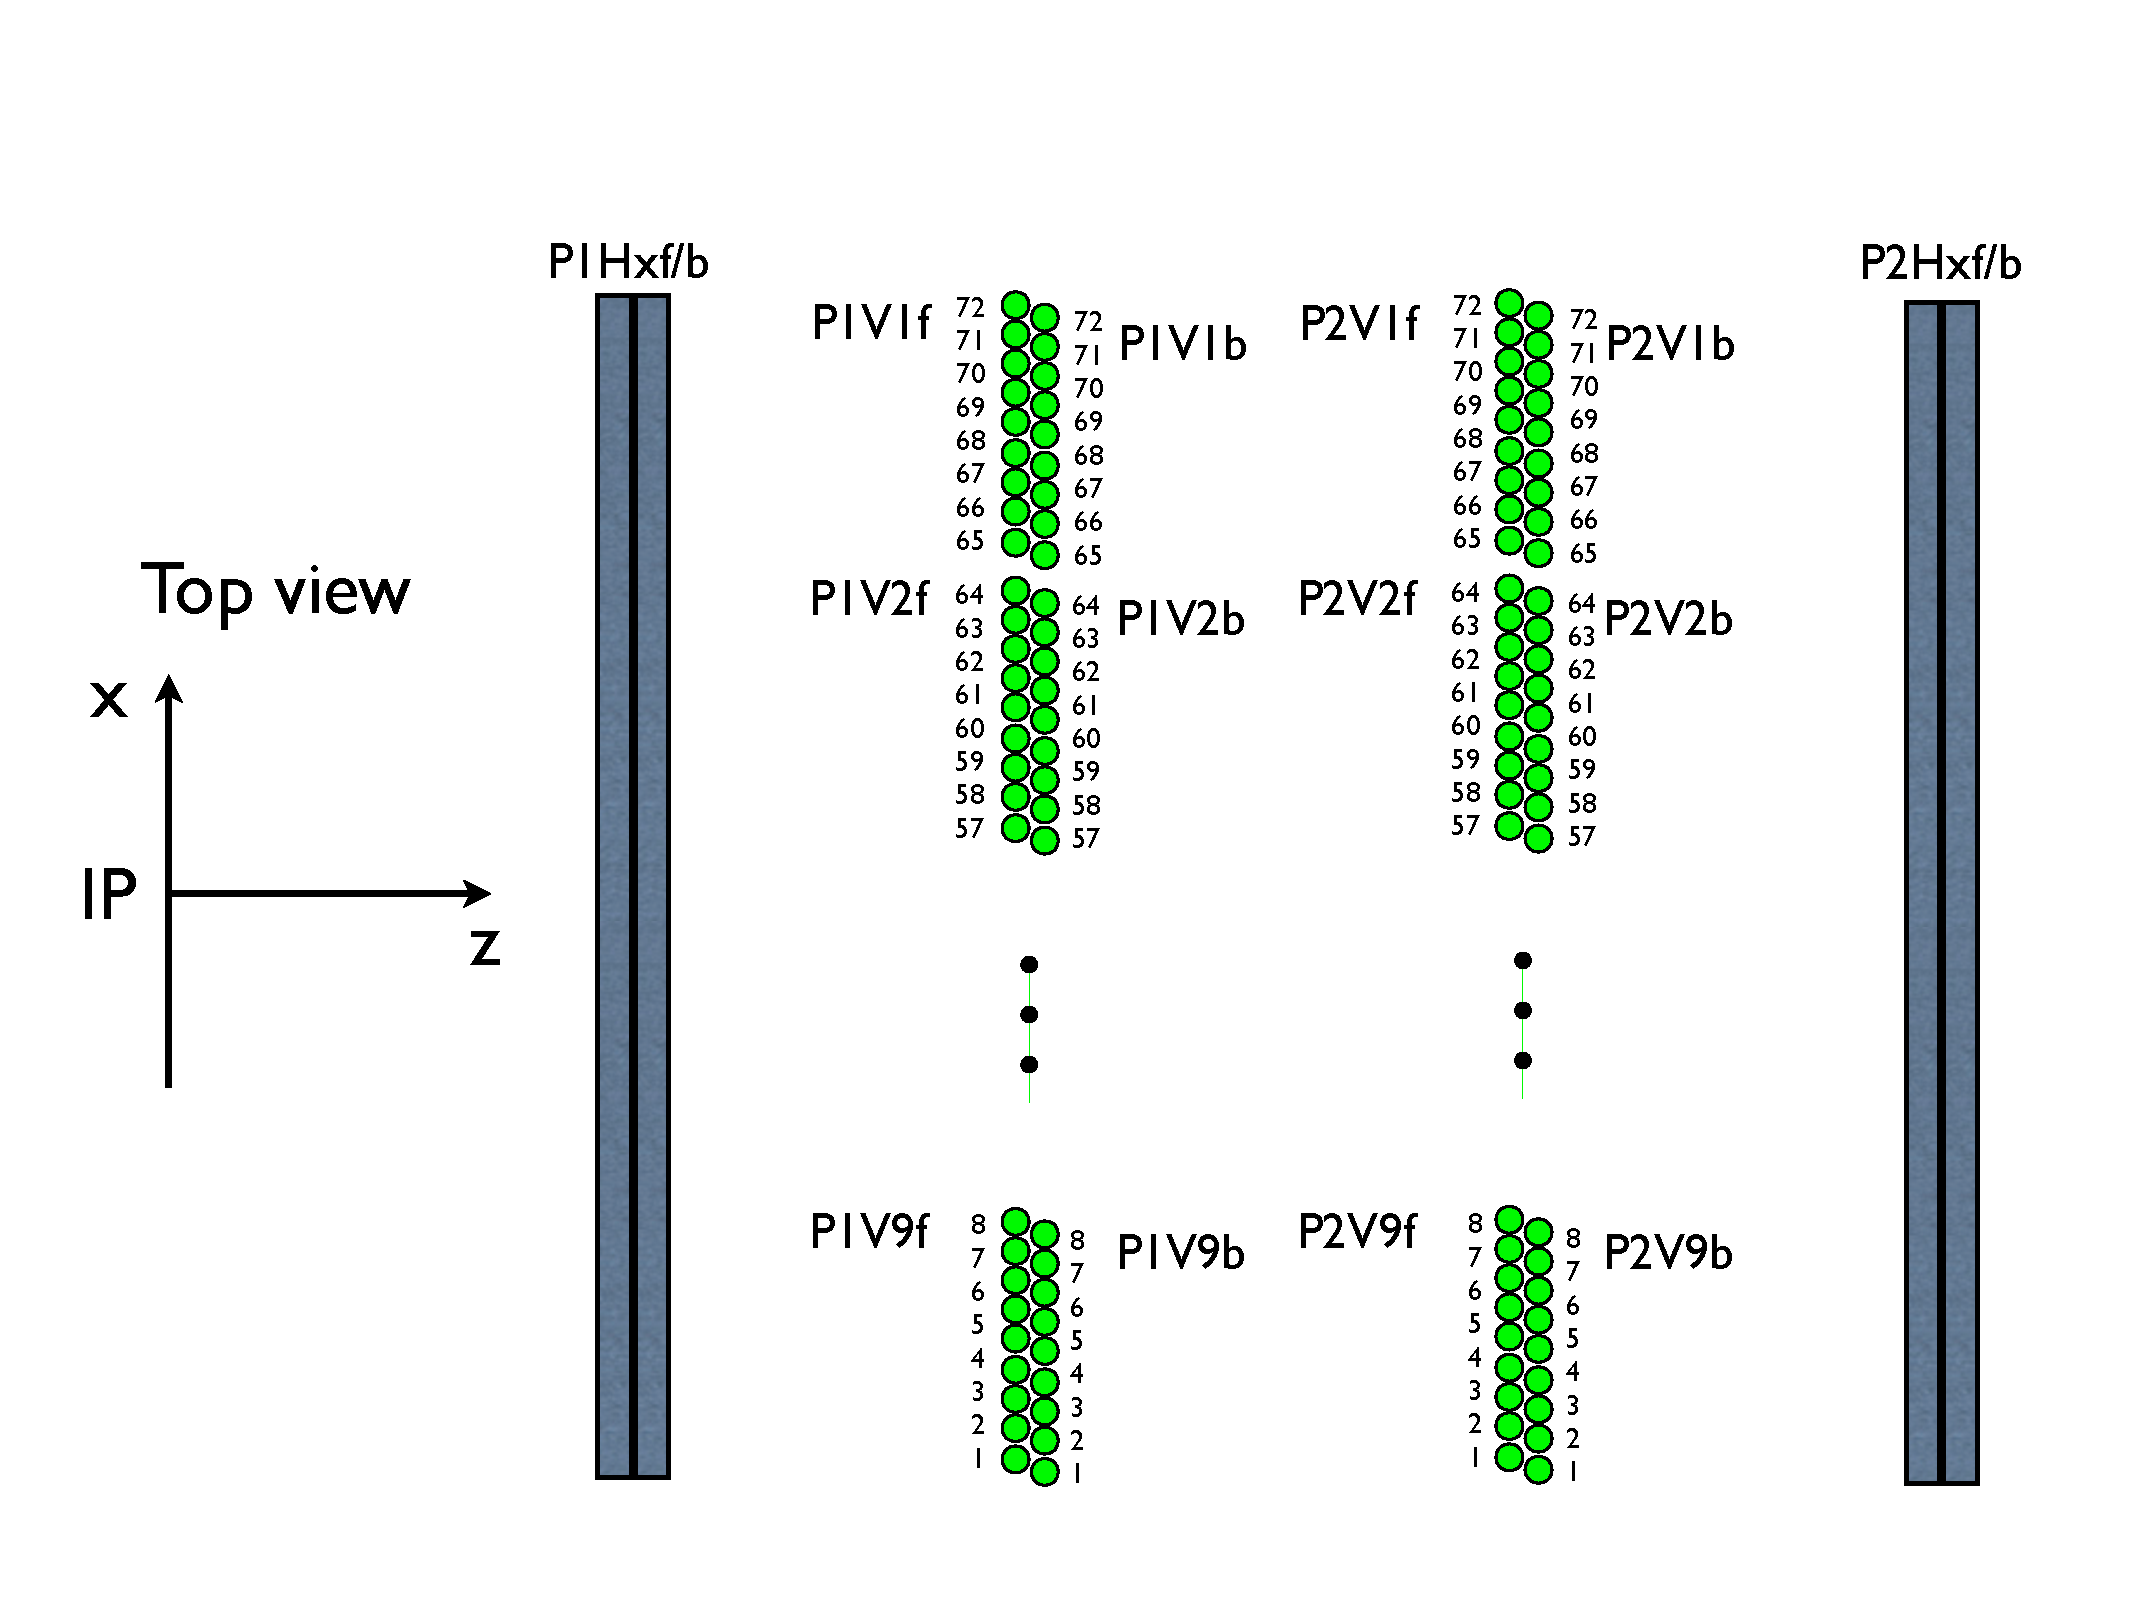
\includegraphics[width=\linewidth]{figures/apparatus/proptubeview_xz.pdf}
		\caption{Proportional tube top ($x-z$ plane) view.}
		\label{fig:proptube:xzview}
	\end{minipage}
	\begin{minipage}[t]{0.49\linewidth}
		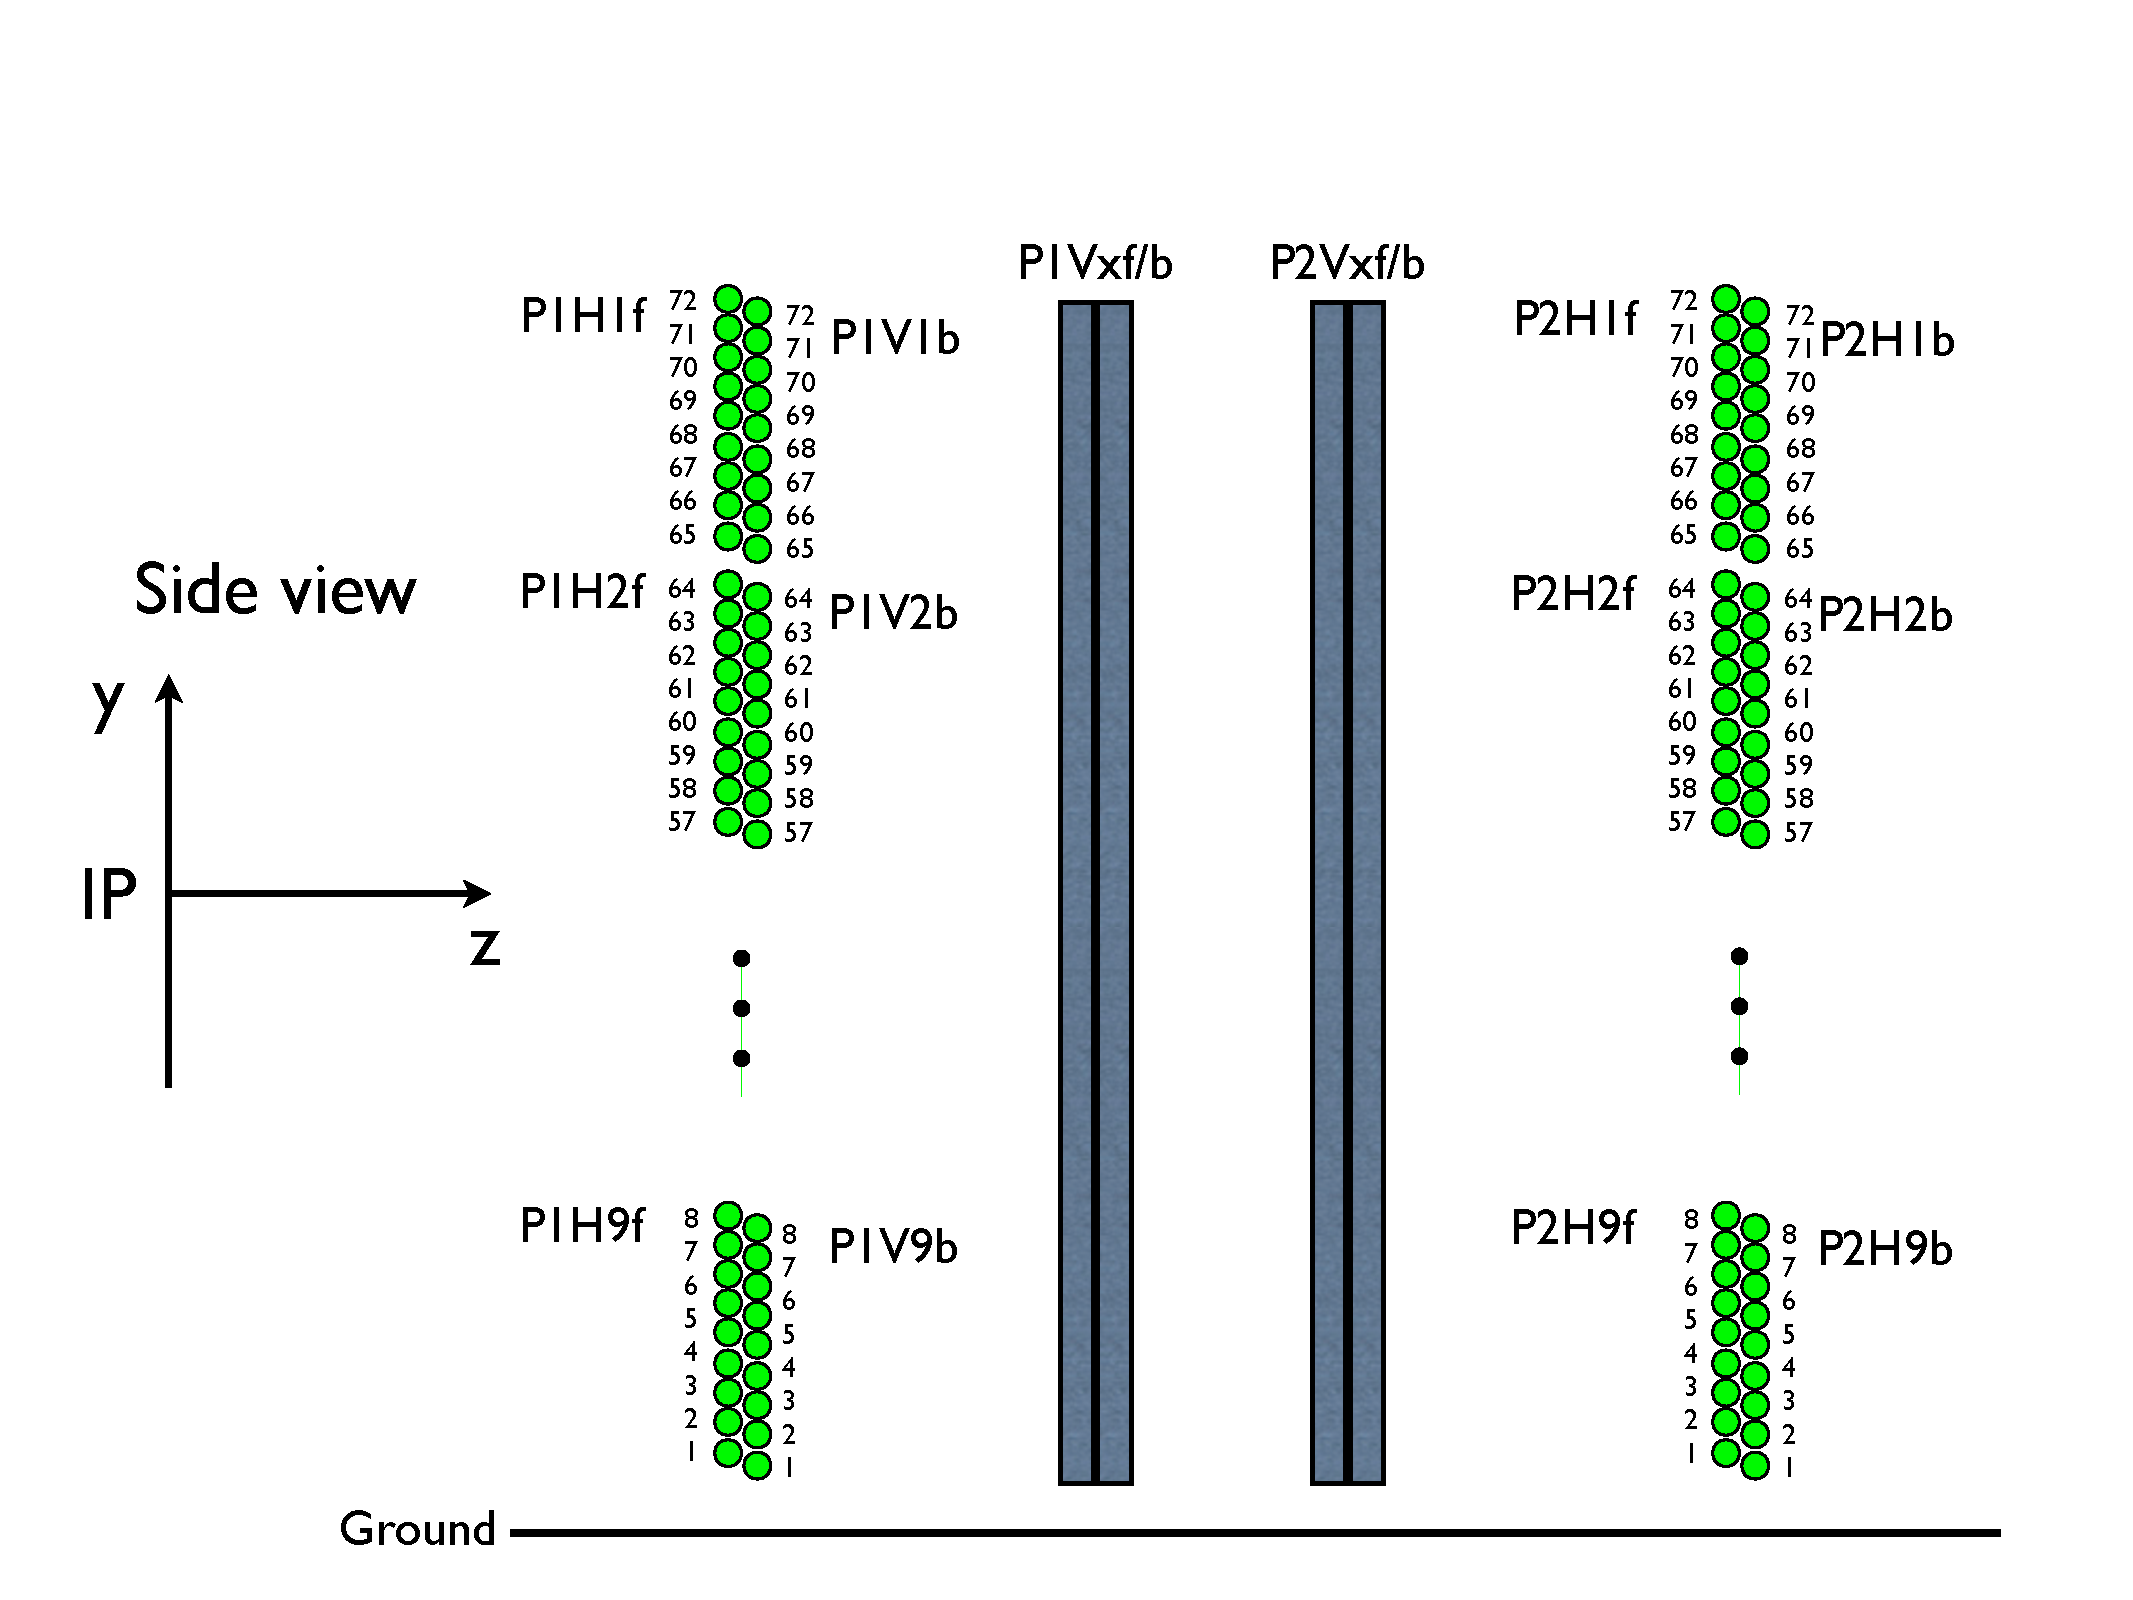
\includegraphics[width=1.03\linewidth]{figures/apparatus/proptubeview_yz.pdf}
		\caption{Proportional tube side ($y-z$ plane) view.}
		\label{fig:proptube:yzview}
	\end{minipage}
\end{figure}

Each plane of proportional tubes is composed of 9 \emph{modules}, each having a set of 16 proportional tubes: 8 in line in a horizontal or vertical orientation and 8 more offset (``primed'') from the first 8 by 0.5 inches. This offset structure prevents any muons from going undetected between tubes and allows for left-right disambiguation for two hits in adjacent primed-unprimed sub-plane pairs in the same module. The modules are labeled $1-9$ in increasing order from left to right for the $x-$measuring planes and from $1-9$ in increasing order from top to bottom. So, the top module of the first vertical plane of prop tubes is P2H1. Additionally, in each module, the primed and unprimed sub-planes are referred to as \emph{f} for ``front'' (facing upstream) and \emph{b} for ``back'' (facing downstream). This substructure can be seen in detail on Fig.~\ref{fig:proptube:xzview} and Fig.~\ref{fig:proptube:yzview}.

A single prop tube is made of 2-inch diameter aluminum tubes with a wall thickness of 1/16 inches. The central anode wire is a gold-plated $20 \mu$m diameter tungsten wire kept at approximately 1.95 kV. Considering the staggered nature of each plane's substructure, one can in principle achieve a spatial resolution of 0.3mm.  During Runs 2 and 3 of data taking, a resolution of 0.5mm for high energy muons was observed, which is more than sufficient for muon identification purpose. The gas mixture for prop-tubes is P-10 (Ar:Methane = 90:10) mixed with a $10\%$ CF4 gas (Ar:CO$_2$:CF$_4$ = 70:20:10) which yields the maximum drift time about 400ns. With this maximum, the prop tubes can handle a singles rate up to 2MHz while normal operational hit rates are typically below 1MHz.

A typical desired high-energy muon within spectrometer acceptance will traverse through two prop-tubes in each plane and induces hit signals on two anode wires. The path of a track is reconstructed from the drift time measured on the two anode output, with a custom TDC board that provides 0.44 ns timing resolution. With the hit information reconstructed from readouts of the forward and backward planes in $x-z$ and $y-z$ direction, precise reconstruction of the track trajectories can be obtained. Ideally, 8 hits from the 4 planes are used to form a track pointing back to the target. If such is the case, a candidate muon track is successfully identified.

\begin{table}[bthp]\centering
	\begin{tabular}{c|ccccc}
		\hline \hline
		Detector & Number       & \# tubes     & Width ($x$)               & $z$-position \\
		Plane     & of modules    & per         & $\times$ height ($y$)      & of front (back)   \\ 
		&                & module      & [cm] $\times$ [cm]        & sub-plane    [cm]    \\ 
		\hline
		P1H    &  9     & 16  & 368 $\times$ 368 &  2,099 (+4)    \\
		P1V    &  9     & 16  & 368 $\times$ 368 &  2,175 (+4)    \\
		P2V    &  9     & 16  & 368 $\times$ 368 &  2,367 (+4)    \\
		P2H    &  9        & 16  & 368 $\times$ 368 &  2,389 (+4)    \\
		\hline
		\hline
	\end{tabular}
	\caption{Parameters of the four proportional tube planes.}
	\label{table:prop:param}
\end{table}

\subsection{Mass Resolution from Chamber Resolutions}

\begin{figure}
	\centering
	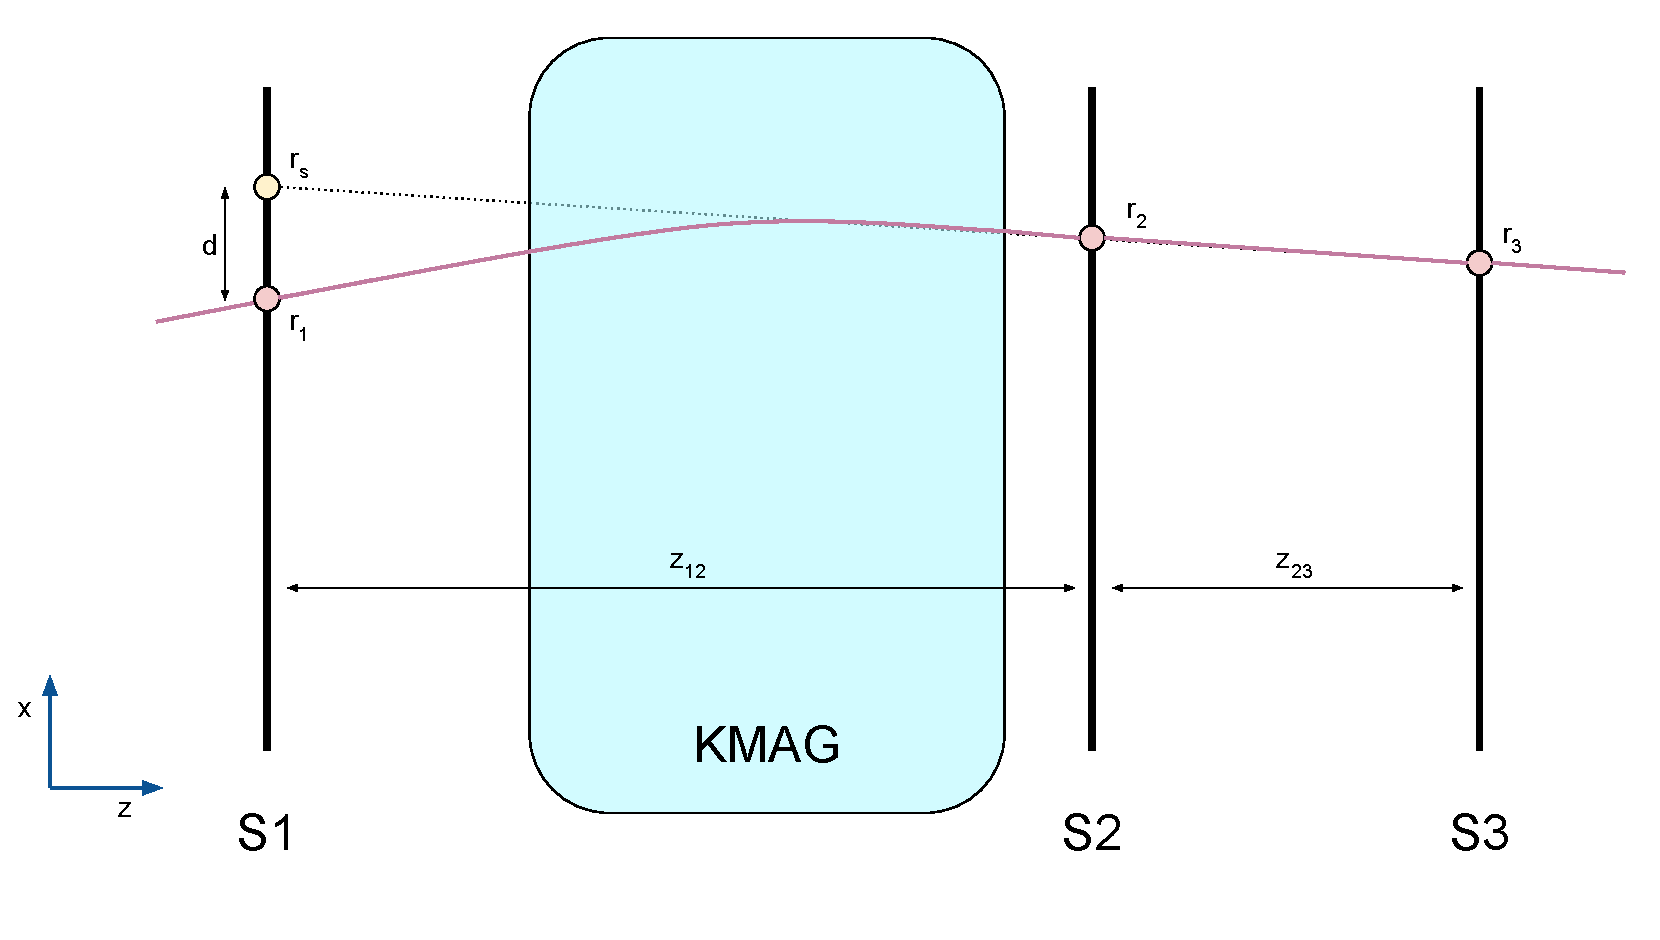
\includegraphics[width=0.75\textwidth]{figures/apparatus/momentum-resolution.pdf}
	\caption{A simplistic depiction of a track passing through from Station 1, through KMAG where its path is bent by the magnetic field, and then straight on through Stations 2 and 3.}
	\label{fig:mom-res}
\end{figure}

The mass resolution of the spectrometer is, in part, limited by the resolution of the tracking chambers and the distances between them. For an arbitrary set of hit positions in Stations 1, 2, and 3 ($r_1, r_2, r_3$) which are separated from each other in $z$ by distances $z_{12}$ and $z_{23}$, with KMAG in between Stations 1 and 2 supplying a $P_{kick}$, one can derive $\Delta P / P$. A line, or track segment, is first reconstructed between $r_2$ and $r_3$. The slope (and its uncertainty) of this track segment in the $z-x$ plane is:
\begin{equation}
s_{23} = \frac{r_3 - r_2}{z_{23}} \ \ ,\ \ \Delta s_{23} = \frac{1}{z_{23}}\sqrt{\Delta r_3^2 + \Delta r_2^2}
\end{equation}
The values of $\Delta r_n$ here are the position resolutions of the individual tracking chambers at each Station. One can use this slope to project a trajectory through KMAG and onto Station 1. The momentum is calculated by seeing where the actual hit position is in Station 1 and looking to the distance ($d$) between where the particle hit the station and where it would have hit had KMAG's magnetic field not existed. This is called a \emph{sagitta analysis}, as the magnetic field moves the particle's trajectory as if along a circle, and we are looking to the particle's path along the sagitta of that circle. Ultimately, the momentum uncertainty is related to this distance as:
\begin{equation}
\frac{\Delta P }{P} = \frac{P}{P_{kick}}\Delta d
\end{equation}
The expected sagitta point ($r_s$) is located at:
\begin{eqnarray}
r_s & = & s_{23} z_{12} + r_2 \\
\Delta r_s = \sqrt{\Delta s_{23}^2 z_{12}^2 + \Delta r_2^2} & = & \sqrt{ \Delta r_3^2 \left(\frac{z_{12}}{z_{23}}\right)^2 + (1+\left(\frac{z_{12}}{z_{23}}\right)^2) \Delta r_2^2}
\end{eqnarray}
And the distance, $d$ follows as:
\begin{eqnarray}
d & = & r_s - r_1 \\
\Delta d = \sqrt{\Delta r_s^2 + \Delta r_1^2} & = & \sqrt{ \Delta r_3^2 \left(\frac{z_{12}}{z_{23}}\right)^2 + (1 + \left( \frac{z_{12}}{z_{23}} \right)^2) \Delta r_2^2 + \Delta r_1^2}
\end{eqnarray}
The momentum resolution due to chamber resolution can therefore be described as:
\begin{equation}
\frac{\Delta P}{P} = \frac{P}{P_{kick}} \sqrt{ \Delta r_3^2 \left(\frac{z_{12}}{z_{23}}\right)^2 + \left(1 + \left( \frac{z_{12}}{z_{23}} \right)^2 \right) \Delta r_2^2 + \Delta r_1^2}
\end{equation}
The dependence of the resolution on $P/P_{kick}$ works such that the larger the $P_{kick}$ is (w.r.t. particle momentum $P$), the more the track is bent, and the more precisely the original momentum is defined. Besides chamber resolution, other contributions to this momentum resolution are from multiple scattering through FMAG's iron beam dump and from the spectrometer's angular resolution. These will be discussed elsewhere in this paper.

The mass resolution is linked to momentum resolution via the following relation
\begin{equation}
\frac{\Delta M}{M} = \frac{\Delta P}{2 P}
\end{equation}
The factor of two arises from the fact that the Drell-Yan dilepton mass comes from two independent muons with the same momentum resolution. This mass resolution is important because it, in turn, contributes to the $\Delta x_2 / x_2$ resolution, which is the key dependent variable for SeaQuest measurements.
\begin{equation}
\frac{\Delta x_2}{x_2} \approx 0.57 \Delta x_F + 0.012 M^2 \frac{\Delta M}{M}
\end{equation}



\section{Trigger}

\begin{figure}
	\centering
	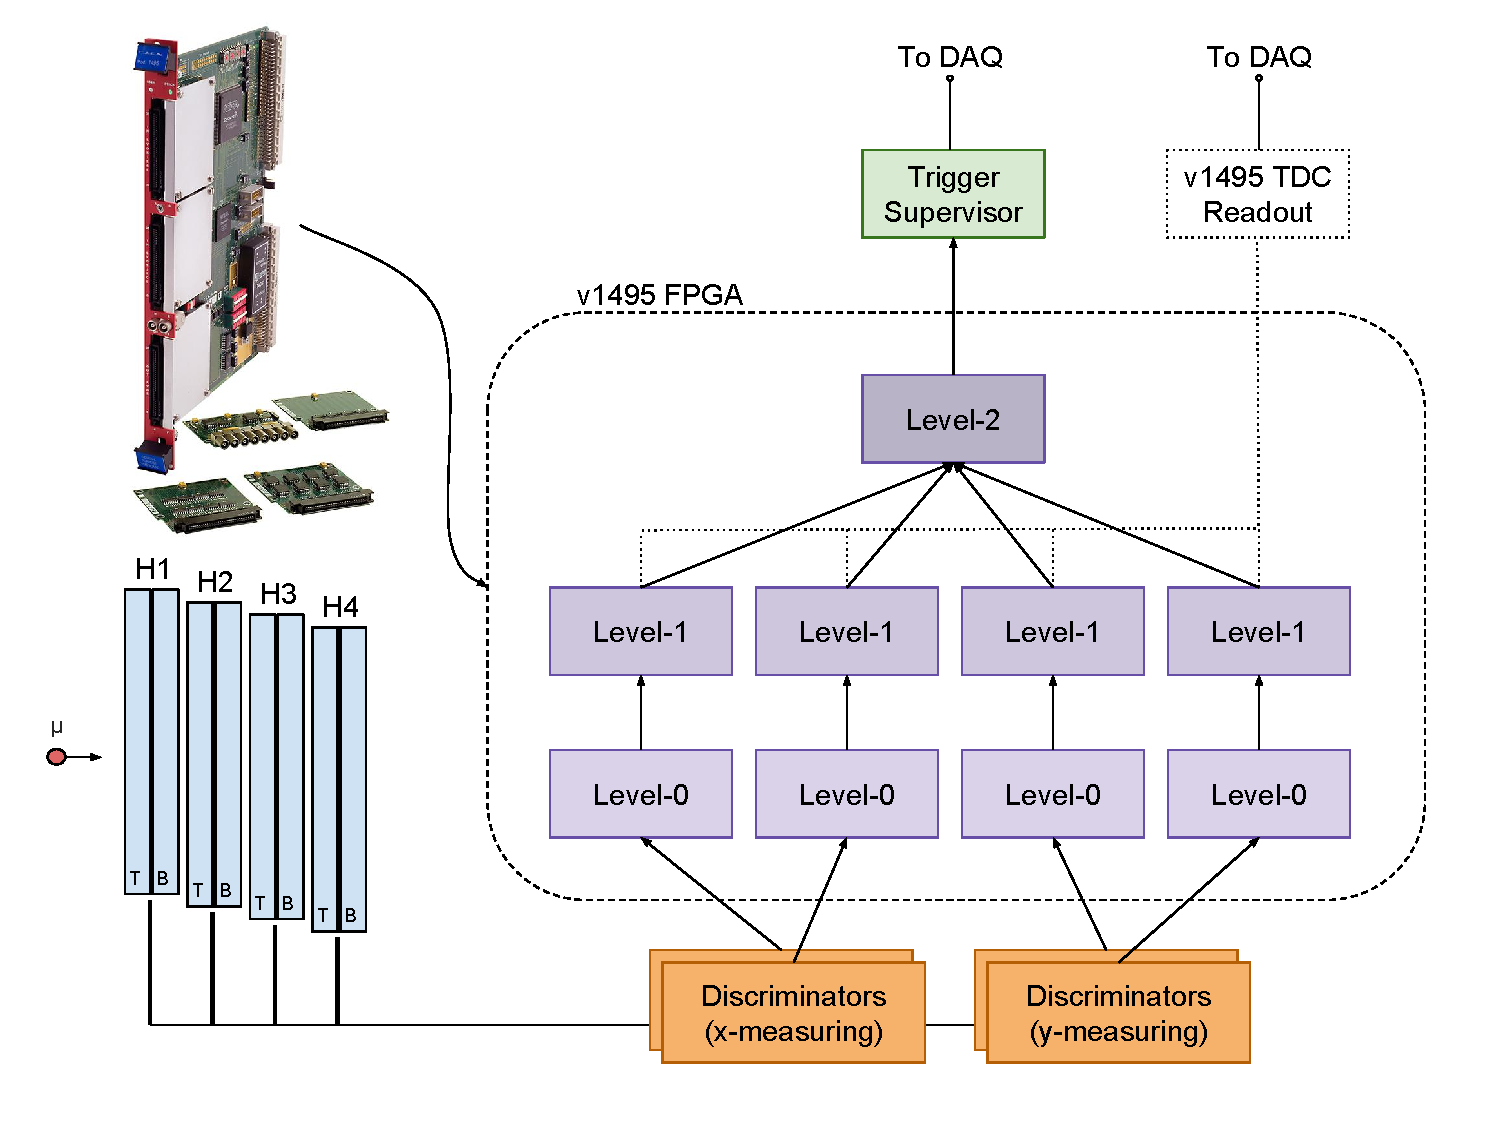
\includegraphics[width=0.75\textwidth]{figures/apparatus/v1495-trigger.pdf}
	\caption{The trigger system at SeaQuest is composed of 9 CAEN v1495 FPGA modules. These modules output a trigger signal to the Trigger Supervisor, which tells the DAQ when to record data.}
	\label{fig:1495-trigger}
\end{figure}

The SeaQuest Trigger System is designed to quickly select candidate dimuon events from the high-rate, high-background environment using discriminated hodoscope signals.

\subsection{Design Requirements}

%% DY selection, trigger rate
The trigger must select events of interest to the main physics goals with good enough efficiency (maximum signal-to-background ratio) to facilitate high-statistics analyses. In general, it is optimized to accept high-mass ($4-10$GeV) dimuons originating from the targets and beam dump. The event selection is also designed to intentionally reduce acceptance of dimuons from other, higher-rate sources, such as $J/\Psi$ decays and non-Drell-Yan dimuons originating from the beam-dump, though enough $J/\Psi$ events are triggered on to allow high-statistics analysis of $J/\Psi$ physics. Other goals of the trigger design are to keep the triggering rate low enough to maintain an acceptable DAQ livetime and to keep the trigger's internal throughput deadtime-free. By design, there should be no bottleneck at this stage, and the trigger should be capable of firing on any and all RF-buckets while the DAQ is live.

%% Flexibility
The hardware, firmware, and design should be sufficiently flexible to quickly accommodate changes in the spectrometer, beam conditions, and physics goals. Any changes to the geometric acceptance of the spectrometer, such as new/moved detectors or changes in the magnetic fields must be immediately reflected in the trigger selection in order to maintain high signal efficiency and good background rejection power. Similarly, a change in the beam duty factor or intensity should be accompanied by a change in the event selection, ensuring trigger rate optimization and zero internal deadtime. Finally, the trigger should be capable of specific modifications to facilitate special runs for other physics goals. For these reasons, the design of the trigger system underscores a significant need for flexibility in its hardware and design.

%% Self-monitoring, transparent
Lastly, the design of the trigger system should include self-diagnostic capabilities, allowing for constant monitoring of the trigger system's performance. Internal pulser-testing is employed to test the function of each compiled firmware every time the trigger logic changes. For added transparency, data from the internal TDC's is used by online and offline software to monitor the self-consistency of the trigger for each recorded physics event.

\subsection{Trigger Hardware}

The triggering system, which is depicted in Fig.~\ref{fig:1495-trigger}, begins with the Stations 1-4 hodoscope arrays. Hodoscopes are used for this task as the time resolution and high speed is limited only by the speed of light through the scintillator paddles and secondary emission of electrons (through the stages of the PMTs. This occurs over the span of nanoseconds, which allows for fast triggering on RF buckets that occur every 19ns during spills. The hodoscope planes - both x- and y-measuring planes - are separated into top and bottom sections as far as triggering is concerned. The signals from the hodoscope arrays are passed through a set of discriminator modules, which will only pass a signal on to the rest of the trigger if there is enough of a signal from the PMT's past a preset threshold.

The output of the discriminators is passed along to one of the nine CAEN v1495 FPGA (Field Programmable Gate Arrays) VMEbus (Versa Module Europa) modules~\cite{caen:v1495}. This hardware trigger consists of a single decision stage with a three-step parallel pipeline. These steps are referred to as the \emph{level-0}, \emph{level-1}, and \emph{level-2} stage triggers. The detailed internal flowchart of the CAEN v1495 electronics can be seen in Fig.~\ref{fig:v1495-internal}.

\begin{figure}
	\centering
	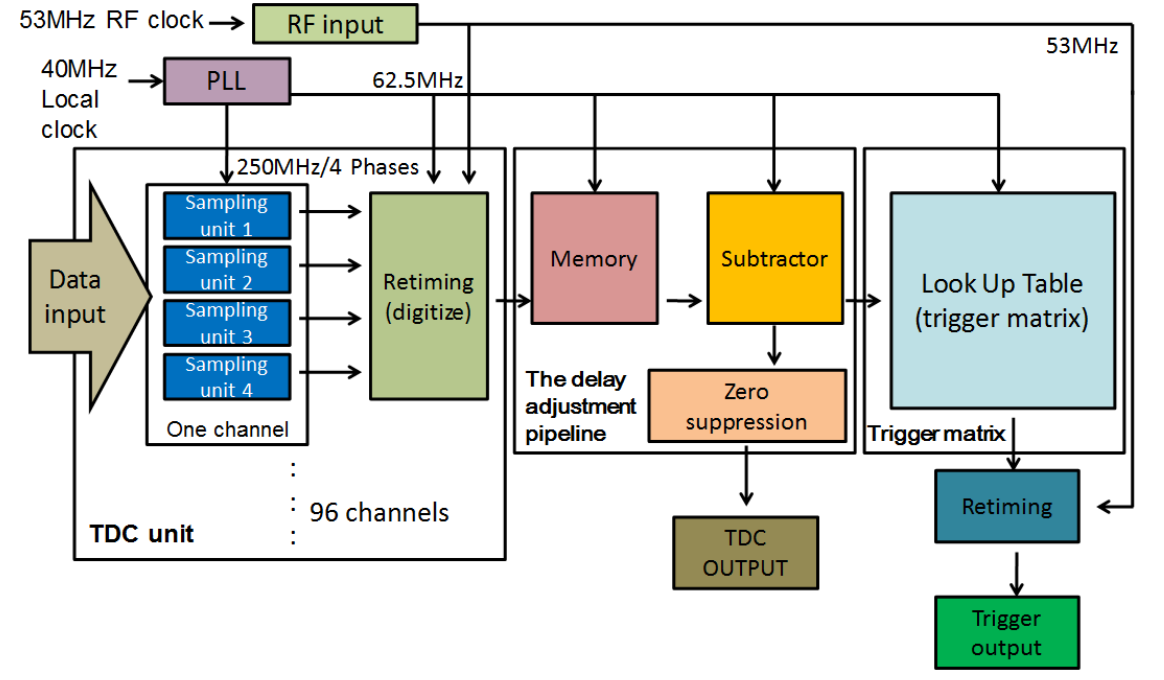
\includegraphics[width=0.75\textwidth]{figures/apparatus/trigger-block-diagram.png}
	\caption{A block diagram of the major functions of the v1495 FPGA~\cite{Shiu:2015ura}.}
	\label{fig:v1495-internal}
\end{figure}

At the first step, level-0, there is nothing actively performed during nominal data taking. The signal is passed on through, unaltered, to level-1. As it stands, level-0 is not used for any of the triggering modes. This stage is, however, extensively used for the pulser testing and self-diagnostic purposes. The level-0 stage is capable of being programmed to pulse arbitrary patterns on to the level-1 stage, which is very useful for observing how level-1 (and subsequently, level-2) will behave in a controlled setting. Whenever a new firmware is installed on the v1495, a pulser test is performed to ensure that all design requirements are met before uploading the firmware for production data taking.

The next level-1 trigger records the hit signals from the x- and y-measuring hodoscope hits split into top and bottom partitions with respect to their location in the SeaQuest spectrometer. The hit patterns are tested via a lookup table against a preselected set of hodoscope hit patterns, or \emph{``trigger roads''}. Each trigger road corresponds to a set of four hodoscopes: one from each station, with all being in the top or bottom half of the spectrometer. In this lookup table, there is a charge and approximate $p_T$ value for each preselected road. These are known via studies of Monte Carlo studies of muon paths from di- or single-muon events originating from the targets or beam dump. The roads were selected such that as many good dimuons are selected while reducing roads that are dominated by background signal that might cause trigger and/or DAQ deadtime.

During data taking, only the x-measuring hodoscopes were used for the v1495 trigger. As such, the two level-1 stages that look to the y-measuring hodoscope signals were unused. The level-1 trigger logic identifies four-out-of-four X1-X2-X3-X4 coincidences, which are characteristic of high $p_T$ single muons produced from the targets or beam dump. Each time a candidate coincidence that satisfies a preselected road is found, the level-1 step outputs certain logical bits indicating the track's charge, detector half (top or bottom), and $p_T$ bin.

The third step of the triggering logic is the level-2 trigger, or the \emph{``Track Correlator''} stage. This step takes the outputs of level-1 (charge, detector half, $p_T$ bin) and finds if any combinations satisfy any of the preprogrammed triggering modes. If one of these modes was satisfied, a signal is sent to the Trigger Supervisor (TS) module that communicates with the DAQ system to record an event at a specific synchronized RF bucket.

\subsection{Triggering Modes}

The v1495 FPGA had five configurable sets of physics triggers were used in the trigger system for the majority of production-level data taking. These five are referred to interchangeably as ``Matrix'' and ``FPGA'' triggers, followed by the number 1-5 indicating which of the five. These modes are described in detail in Table~\ref{tab:trigger-settings}.

\begin{table}[bthp]\centering
	\begin{tabular}{c|cccl}
		\hline
		Trigger & Condition       & Sign    & \#$\mu$ & Prescale\\
		\hline
		FPGA-1   & $T \land B$                        & Opposite  & 2        & 1    \\
		FPGA-2   & $(T \land T)\ \lor (B \land B)$  & Opposite  & 2        & 1000 \\
		FPGA-3   & $T \land B$                        & Same        & 2        & 123  \\
		FPGA-4   & $T \lor B$, all $p_T$            & $+ \lor -$& 1        & 30000\\
		FPGA-5   & $T \lor B$, $p_T > 3GeV$            & $+ \lor -$& 1        & 2000 \\
		NIM-1    & Y-coincidence                     & NA        & NA    & 30000\\
		NIM-2    & X-coincidence                    & NA        & NA    & 1000 \\
		NIM-3     & Random RF                        & NA        & NA    & 1000 \\
		\hline
	\end{tabular}
	\caption{Trigger settings for Run 3 and beyond. Prescale figures shown are typical values and were adjusted as experimental needs were tuned. NIM-1 and NIM-2 triggers' exact conditions could be changed and reconfigured from the counting room.}
	\label{tab:trigger-settings}
\end{table}

Different trigger settings were used for capturing data for different purposes. The primary triggering mode is FPGA-1, which looked for a combination of two roads of opposite sign that reside in opposite halves of the spectrometer. The FPGA-2 looked for good muon pairs that occurred in the same half. This, however, turned out to have a combinatoric problem that had two adverse effects: track reconstruction was difficult for these types of events, and the trigger fired off too often, causing high trigger and DAQ deadtime. As such, FPGA-2 was disabled for much of data taking. FPGA-3 trigger looked for the same kind of signal as FPGA-1, but with same-sign muon pairs. This type of event is useful for analyzing the experiment's combinatoric background. FPGA-4 and -5 are ``singles'' triggers that record events that are useful for estimating backgrounds and detector efficiencies. Each of these has a \emph{``prescale factor''} that limits how many of each mode actually fires the trigger. For example, FPGA-3 has a prescale factor of 123, which means that, within a single spill, there must be 123 FPGA-3 events before it tells the DAQ to record one. This keeps certain high-frequency trigger modes from dominating the readout and causing undue deadtimes.

In addition to the v1495 FPGA triggering mechanism, the outputs of the hodoscope discriminators are also sent up to the control room to a set of NIM logic modules. These signals, however, do not describe each hodoscope paddle but instead are \emph{AND}s of the tops and bottoms of each plane. For example, if one or more paddles in H1T fires, then a positive signal is sent out indicating that H1T fired. These signals can be used to form a rudimentary trigger on situations such as 4- or 3-out-of-4 coincidences in the X- or Y-direction hodoscope planes. In general, NIM-1 is used for Y-coincidences, and NIM-2 is used for X-coincidences.

The third NIM trigger mode is of particular importance, as it is used for estimating a great deal regarding backgrounds and rate dependence issues. The NIM-3 trigger is called the ``Random RF'' trigger, as it is controlled by two different clocks beating against each other. When the two clocks are in coincidence, they will send a signal to the Trigger Supervisor to record the event corresponding to the next immediate RF bucket. This trigger allows the experiment to get a random sample of the events that are occurring at the spectrometer, notably without a bias that a selective trigger can incur.

\section{Data Acquisition Systems}

The whole of the SeaQuest experiment spans two sectors of the NM beamline (NM3 and NM4) and records not only detector data but also accelerator and atmospheric conditions. Designing a data acquisition (DAQ) for this experiment, therefore, requires a bandwidth and timing which cannot be provided by a single central computer system. SeaQuest has therefore employed four separate DAQ subsystems called ``Main DAQ'', ``Scaler DAQ'', ``Beam DAQ'' and ``Slow Control''. The Main DAQ records the main detector information and the trigger timing. Scaler DAQ records various scaler readouts once per spill to reduce bias from the dead time of Main DAQ. Beam DAQ records information from a beamline \v{C}erenkov detector read out by its QIE board. The Slow Control is a catch-all for everything else, from magnet current to radiation monitors that are read out once per spill.

\subsection{Main DAQ}

The MainDAQ is powered by a Jefferson Lab developed software package named CODA (CEBAF\footnote{The old acronym inside of an acronym bit. CEBAF: Continuous Electron Beam Accelerator Facility} On-line Data Acquisition). The Trigger Supervisor could receive up to 12 different kinds of triggers. The first four triggers (FPGA 1-4) can be prescaled up to 24 bits. The second four triggers (FPGA 5, NIM 1-3) can be prescaled up to 16 bits. The rest of triggers (NIM4, flush trigger, Beginning of Spill (BOS), End of Spill (EOS)) are not prescalable. The Main DAQ can configure which triggers are enabled at the Trigger Supervisor level and what the  prescale factors are for each triggering mode. Once the TS receives a trigger, it will count the prescale factor and, based on how many triggers of that type have fired so far, it will decide if the Main DAQ will accept the trigger or not. 

Once the TS accepts the trigger, it sends an ``accepted trigger'' signal to the other front end electronics, such as the detectors' TDC readouts. Facilitating intercommunications, the Main DAQ system is connected to the TS and the CPU's in the VME crates via a local network. These CPU's are known colloquially at SeaQuest as readout controllers, or ``ROC's''. The TS connects with each VME crate, and when the TS sends an ``accepted trigger'', an interrupt signal is sent to each of the ROC's. The ROC's will then start reading the various front-end electronics (FEE).

The TS also sends a signal to the to QIE of the BIM, and the QIE retains information regarding the $\pm$16 RF buckets around that triggered RF bucket to assist in investigating the beam quality around each of our event triggers. The output of the QIE is encoded into a scaler latch card format. If the beam intensity in RF buckets neighboring the trigger is higher than the user-select threshold, then the board will issue a veto signal to the TS to ignore this trigger.

The Main DAQ's deadtime is considerable, as it has to communicate with the TDC's, which have the longest copy-in-progress time of \unit[32]{\us}. The average TDC readout time is approximately \unit[300]{ns} per 32bits (one hit), and as such, the slowest ROC which contains 7 TDCs has, on average, \unit[150]{\us} deadtime. This deadtime is accounted for under the umbrella term of \emph{``busy''} time and factored into the calculation of the ``live protons'' received by the experiment.

\subsection{Scaler DAQ}

The Scaler DAQ is used to ensure that the detector and trigger systems are working properly. The readout controller CPU is an MVME5500~\cite{mvme:scaler} with four scalers. One of these scalers is triggered by the coincidence of a \unit[7.5]{kHz} gate generator and the beam spill signal. This records the \unit[7.5]{kHz} response of the hodoscope arrays. The other three scalers are triggered by the BOS or EOS signals and thus record spill-level rates. Data collected by these spill-level scalers are the number of times each Main DAQ trigger is satisfied (both raw and accepted), the intensity of the beam, and the rates of the hodoscope arrays. The readout of this VMEbus DAQ is done using CODA very similarly to the Main DAQ but on a completely different system. An independent program analyzes the data in real-time in order to monitor the performance of the detectors and triggers, as well as the quality of the beam. 
%%An example of the ever-present online set of Scaler DAQ plots can be seen in Fig.~\ref{fig:scalerdaq}.


\subsection{Beam DAQ}

The Beam DAQ is composed of a \v{C}erenkov detector in the proton beam (the Beam Intensity Monitor discussed earlier in this chapter), a QIE board, and a custom C++ program to control their operation and read out. The Beam DAQ is responsible for recording the \unit[53]{MHz} structure of the beam, i.e. the intensity of each RF bucket. Its calculation of the \unit[53]{MHz} duty factor $DF=\frac{<I>^{2}}{<I^{2}>}$ is the primary measure of beam quality that accelerator operators use for tuning. In short, the duty factor is a measure of the \emph{uniformity} of the intensity of the beam. If we were to ignore the buckets intentionally left empty, and if it were to be the case that every RF bucket had the same number of protons, the \unit[53]{MHz} duty factor would be 100\%.

There four types of data recorded by the QIE have already been covered in the Beam Intensity Monitor section: QIESum, beam inhibit, busy time, and the $\pm16$ RF bucket intensities. The Beam DAQ commences read out of each of these blocks of data when the EOS signal is seen. The block of QIE data for all buckets is about \unit[300]{MB}. To read this much data in time to analyze it and be ready for the next spill, the DAQ program utilizes multithreaded processes. Three threads are used to read the data from the QIE board's three ethernet chips, and up to eight threads are used to analyze the data. Analyzed data is displayed on a public webpage so that shifters and accelerator operators can monitor the quality of the beam (Fig.~\ref{fig:beamdaq}). The fully processed data is also written out to tab-delimited ASCII files, which are archived and also uploaded to our online MySQL server.

\begin{figure}
	\centering
	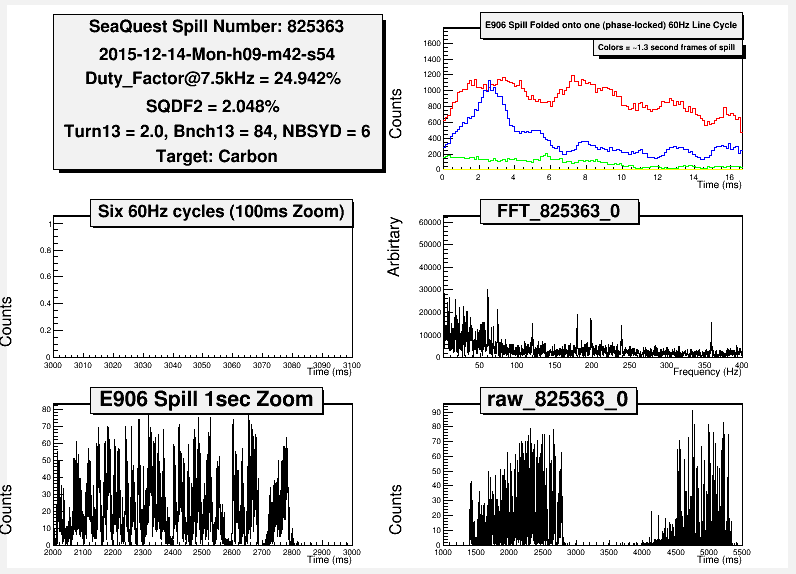
\includegraphics[width=0.75\textwidth]{figures/apparatus/E906FFT-scalerDAQ.png}
	\caption{A standard Beam DAQ display showing beam characteristics and spill data. The bottom two plots show the output of the QIE on a \unit[]{ms} scale.}
	\label{fig:beamdaq}
\end{figure}

\subsection{Slow Control Readout}

The Slow Control readout system is an aggregation of many different readouts from various parts of the experiment. This is also the umbrella term for other critical monitoring and bookkeeping tasks that must be performed. The one common thread to them all is that they only \emph{need} to be read out / performed once per spill in order to give perspective on the conditions of the experiment for each given spill. The term \emph{``Slow''} in Slow Control is adapted from the term ``Slow Spill'', which is used to characterize the method of beam delivery to SeaQuest. The Slow Control is run by an array of Python, Perl, and Bash scripts that, for the most part, run independently. These scripts primarily interact with and read out from EPICS, ACNET, and the local Spill Counter.

\subsubsection{EPICS, ACNET, and Kiethley}

The EPICS software package (Experimental Physics and Industrial Control System) is used for communicating any number of variables across the experiment's local network. EPICS is used for feeding readouts from many different sources and formats, and making them available to any other system that may have need of certain information, but does not natively communicate with a different system's format. Bridging this gap, EPICS is able to gather information regarding the target, beam, and environmental data into one place.

The EPICS server is installed on SeaQuest's target control computer, where the target position, pressures, temperatures, and proximity sensors are monitored and controlled. These values are critical to track and monitor, as they affect what target is in position at any given spill, along with information that may infer the cryogenic liquid targets' densities. Additionally, there is information regarding the operational mode of the target table, such as whether or not the target table is being manually controlled or if it is automatically repositioning itself. In Slow Control parlance, information from the target computer that is sent to the EPICS server is labeled as ``Target'' type data.

Several values are read into the EPICS server from the Accelerator Network (ACNET), which monitors many critical systems. Beam intensities (S:G2SEM) and FMAG / KMAG currents are two of the major factors that must be factored in for any analysis. There are additional readouts with esoteric names that can record anything from beam pipe vacuum to upstream radiation monitors. It is important to note that the FMAG and KMAG variables from ACNET are read out to the EPICS server every \unit[3]{s}, particularly because it is unsafe to deliver beam to the sensitive detectors without FMAG being fully powered. As such, the FMAG current is read into the beam interlock system. In the Slow Control feed, this type of information is labeled as ``Beam'' data.

Finally, there is a Keithley multimeter \CN in SeaQuest Hall near the electronics racks by Station 3. This device has the responsibility of relaying information regarding ambient temperature, air pressure, and humidity up to the control room. This information on its own is not typically used for any analyses, but in the case that, for example, a rise in humidity results in any electrical device failures, the monitoring data exists to diagnose it as such. This data is gathered by a `kscan' program that is run on the target machine, and its operation typically takes 11s to return a result. Data from the Keithley multimeter that is put into the Slow Control feed is labeled as ``Environment'' data.

\subsubsection{Spill Counter}

Perhaps one of the most critical components of the data acquisition is the coordination between the many sources of data in the DAQ. The Main DAQ, Scaler DAQ, Beam DAQ, and Slow Control do not share a single clock or network, so some measures need to be taken to ensure that data from different sources regarding a single spill's worth of data actually all correspond to the same spill. The concept of a locally maintained Spill Counter arose as a solution to this problem, and it is handled in the form of a simple Python script and a flat text file containing a single integer.

The enacted solution begins with placing an initialized spill counter (\emph{spillID})value (currently \emph{O}($10^5$)) into an otherwise empty text file at a specified location. Then, when the ACNET readout receives a BOS/EOS signal from AD, a simple python script performs the following:
\begin{itemize}
	\item Read the current spillID from the file
	\item Broadcast this value over the EPICS server
	\item Insert a single ASCII-encoded event into the Main DAQ and Scaler DAQ CODA streams containing only that spillID number
	\item Waits for \unit[20]{s} while other scripts may want to use the current spillID value to connect its value to the spill that just ended
	\item Updates the file to contain spillID + 1
\end{itemize}

This simple approach has been very effective in its usage so far, and the spillID incremented via this method has been shown to be accurate upon scrutiny of data contents across DAQs. This can be easily done by looking at a series of full and empty spills, as it is obvious which spills had a nominal beam spill and which did not by investigating the output of each DAQ. The weakness lies in the fact that this system relies on a single file, which is susceptible to any number of file access and timing issues. At some point in the future, it would be advisable to have all spillID-using systems to read the current value from the broadcasted EPICS server value instead of having several applications attempting to access and read the single file (even if just read-only).

\subsubsection{Python Slow Control Script}

With all of this going on to aggregate data from several sources, there is one final script that takes this aggregated data and makes it readily available for the rest of the DAQ systems. A \verb|read_slowcontrol.py| script, once every \unit[60]{s} supercycle, puts the following together into a single ASCII text file:
\begin{itemize}
	\item Clock time (``vxticks'') of the Trigger Supervisor
	\item Spill count data
	\item Beam data
	\item Environmental data
	\item Target data
	\item Timestamp
\end{itemize}

Once all of this is written to a file, this is sent to the Main DAQ and Scaler DAQ to be integrated into the full CODA file as a plain text event with a simple, tab-delimited format.
%\chapter{Photomultiplier Tube Base Upgrade}

\begin{figure}
	\centerline{
		\mbox{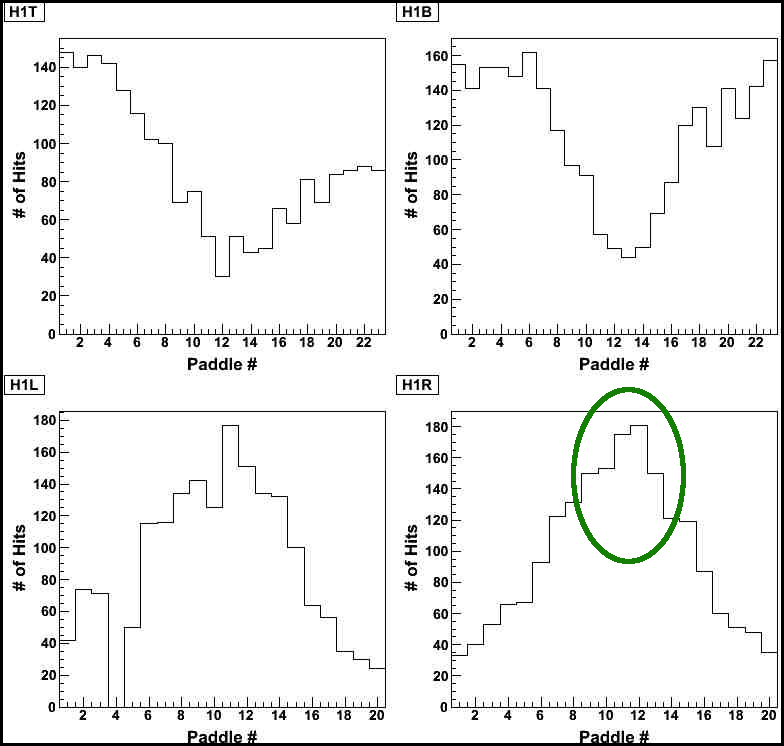
\includegraphics[width=0.5\textwidth]{figures/pmtupgrade/nosag.jpg} 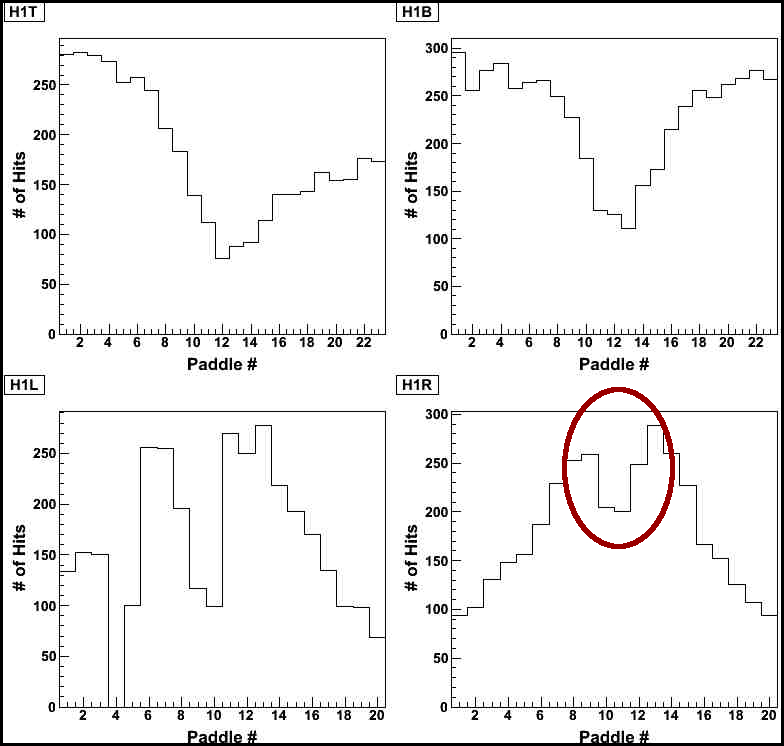
\includegraphics[width=0.5\textwidth]{figures/pmtupgrade/sag.jpg}}
	}
	\caption{(Left) Histogram of hodoscope `hits' in a typical event; (Right) Histogram of high-intensity event, with marked sagging most noticeably in the middle of the y-measuring hodoscopes}
	\label{fig:sag}
\end{figure}

During Run I of SeaQuest, observations of hodoscope wire maps (as in Fig.~\ref{fig:sag}) suggested an apparent drop in expected performance in the $y-$measuring hodoscopes. While this performance was most obviously seen in the $y-$measuring hodoscope planes, the $x-$measuring planes were likely also affected. This effect was assumed to be due to high-intensity RF buckets that caused very high multiplicity in all of the detectors in the spectrometer for that event. The result of these intense events seemed to push the PMTs and/or their PMT base electronics past their operational capacity.

The understood cause of this \emph{``sag''} in performance, as it came to be called, was due to a destabilization in the voltage divider in the PMT base. This critical component holds each dynode stage at a specific voltage, and when this destabilizes and is unable to maintain an appropriate voltage difference between dynode stages, inefficient performance of the PMT results.

During the Fall of 2012, prototyping and testing were performed with the goal in mind being to assemble a new base for the Philips XP-2008 PMTs~\cite{tubespecs} and compare its performance to the original PMT base and to some modern, high-performance Hamamatsu PMTs. Once a base design tested well, the new bases would be manufactured and installed in the existing frames of the original PMT bases.

\section{PMT Basic Construction and Operation}

\begin{figure}
	\centering
	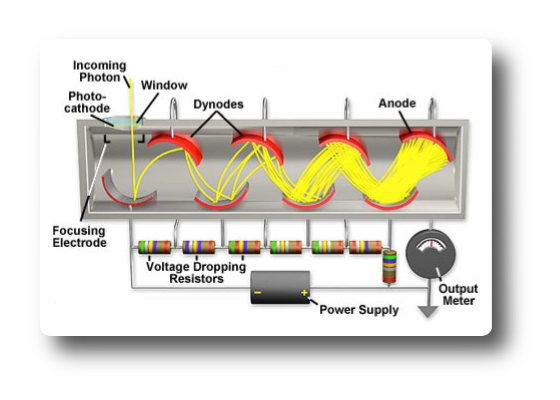
\includegraphics[width=0.7\textwidth]{figures/pmtupgrade/pmt-diagram.png}
	\caption{A diagram of typical PMT operation. The circuit controlling the voltage-dropping resistors is the part that was upgraded in this chapter.}
	\label{fig:pmt}
\end{figure}

Figure~\ref{fig:pmt} shows a schematic design of a typical photomultiplier tube and base setup. It consists of a photocathode that is followed by an electron multiplier section (or dynode string) then an anode from which a final signal is delivered. During operation, a high voltage is applied to the photocathode, dynodes, and anode in such a way that there's a potential ``ladder'' going from stage to stage. When an incident photon from the hodoscope scintillator paddle hits the photocathode, an electron is emitted via the photoelectric effect~\cite{Einstein:1905cc}. The voltage difference between the cathode and dynode stages draws the emitted electron to the dynodes, and each time an electron hits a dynode, some of that electron's energy is transferred to other electrons in the dynode. These electrons then are emitted and become accelerated towards the next dynode stage. This process is called secondary emission, and by the time the process is repeated, there is a cascade or avalanche of electrons that land on the anode, resulting in a signal that can be amplified and analyzed.

It is the case that the voltage divider ultimately supplies the electrons that are emitted in this signal cascade. If too many photons and resultant electron cascades occur, the dynode stages' voltage divider will destabilize as they attempt to resupply the dynode stages with electrons. The problem that was experienced at SeaQuest was that these high-intensity events were flooding the PMTs with photons, causing this ``saturation'' which caused this destabilization and the inefficient performance that was observed. The goal specifically was to test out modern base designs that provided for added stability to the performance of the voltage divider, even under high rates.

In general, each base divides around a \unit[-1500]{V} potential total over the photocathode (K), ten dynode stages (D1-D10), and the anode (A). There are two currents that are referred to here:
\begin{itemize}
	\item Signal Current: This is the signal that passes over the anode, which is the end-result of the cascading secondary emission electrons from each dynode stage.
	\item Bleeder Current: This is the current through the voltage divider. It is termed the ``bleeder'' current since the compounding electrons in the signal current must be ``bled'' from the current through the voltage divider.
\end{itemize}

Throughout these voltage base designs, capacitors are commonly implemented in the latter dynode stages where the most electrons are emitted. These capacitors, when charged, are able to replenish the lost charge on its corresponding dynode stage in the event that an intense light pulse induces a large signal current.  As the capacitor is able to hold its own charge, this resupply can occur without requiring the charges to be drawn from the bleeder current, thereby keeping the voltage across the dynode stages more stable.

\section{PMT Base Design Iterations}

There were several iterations of base design to determine which was best to approach for full base production and installation at SeaQuest. The core addition was the inclusion of transistors between dynode stages, according to the improvements suggested by C.R. Kerns in his paper regarding high-rate PMT bases~\cite{Kerns:1977qr}. Common solutions to destabilization in PMT bases have been to have (1) very large capacitor banks with charges $> 10^3$ times greater than the time-averaged dynode current and/or (2) miniature on-board, separately-powered Cockroft-Walton power supplies for the final dynode stages. A Kerns-style transistorized base allows for a light-weight, small size, and simple base that does not require extra power supplies or voluminous energy storage capacitors.

In general, there are three important features that were tuned in this set of prototypes that affected the performance of the phototubes:
\begin{itemize}
	\item
	Lower resistance
	\item
	Transistors (with protective diodes)
	\item
	Higher capacitance between dynode stages
	\item
	Distribution of voltage division
\end{itemize}

The lower overall resistance of the voltage divider increases the bleeder current. This means that the base will be more capable of handling high-intensity, as it will be better able to replenish the charges on each dynode stage in the case of a large signal. Typically, the larger the bleeder current, the larger the signal current can be without destabilizing the voltage divider. Higher rates usually put higher demand on the signal current, so by reducing the overall resistance, one can easily increase the rate capability. The shortfall here is that with voltage constant and resistance decreased, according to Ohm's Law ($V = IR$), the current will increase. As a result, the power dissipated by the circuit ($P = I^2 R$) will go as $I^2$, and the PMT base may heat up to critical temperatures faster than it can dissipate the heat as there is no significant ventilation in the PMT base enclosure. The Philips XP-2008 manual quotes that for continuous usage and storage the ambient temperature should not exceed $50^\circ C$ ($122^\circ F$). In addition to heat concerns, there's typically a power rating for the class of small on-board resistors that were planned to be used. Approaching or exceeding that power limit would run the risk of burning out a resistor and rendering the base inoperable. 

\begin{wrapfigure}{L}{0pt}
	\centering
	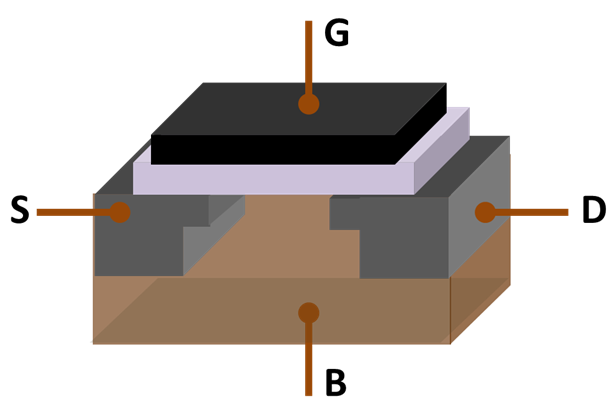
\includegraphics[width=0.4\textwidth]{figures/pmtupgrade/MOSFET_Structure.png}
	\caption{MOSFET showing gate (G), body (B), source (S) and drain (D) terminals. The gate is separated from the body by an insulating layer (white)~\cite{wmc:mosfet}}
	\label{fig:mosfet}
\end{wrapfigure}
The use of a specific type or micro-transistor, a metal–oxide–semiconductor field-effect transistor (MOSFET), is introduced here to maintain the proper voltage division. In general, MOSFET transistors have an \emph{source}, a \emph{drain}, and a \emph{gate}, where current flows freely through from the source to the drain, gate permitting (Fig.~\ref{fig:mosfet}). If at any point a certain voltage across the gate of the transistor is not supplied (here, the voltage across dynode stages), then the source-to-drain current through the transistor is stopped until the proper gate voltage is restored. This helps greatly to ``intelligently'' regulate the voltage across the dynodes. Wherever transistors are used, diodes are also implemented to prevent the unlikely case of a current moving across the transistors' gate in the wrong direction. This protects the transistors from being damaged particularly when powering the circuit on and off.

Having capacitors along the higher dynode stages allows for a quick resupply of charges to the dynodes, thus maintaining proper voltage division. This, however, is only a stop-gap measure and is only effective in cases of high instantaneous currents. It is the case that, should there be a constant too-high rate of operation, the capacitors will not be able to recharge themselves. Typical recharge time for the capacitors discussed in this section can range from \unit[0.1-1]{ms}.

Finally, the specific division of voltage across each stage, from D1 to A, has an influence on the behavior of the PMT operation. As we see from the operations manual of the phototube in Fig.~\ref{fig:voltage_schemes}, in the case of a progressively increasing voltage division, there is a good compromise between timing and linearity. With respect to phototube operation, ``linearity'' is the quality that the amount of charge deposited on the anode is linearly proportional to the energy of the incident photon. ``Timing'', on the other hand, is the quality that the time it takes for a high-energy photon signal and a low-energy photon signal to progress through the stages should be the same. For the purpose of optimization at SeaQuest, we wish to optimize the amount of signal (i.e. amplification or \emph{gain}) that the phototube can accommodate. For this, the recommended voltage partitioning is flat from D1-A~\cite{tubespecs}.

It should be noted that the prototype iterations of PMT base design changes were not intended to cover the entire phase space of these tunable parameters. The purpose of these tests was to get a sense of how changing one or more of these parameters could affect the PMT high-rate capabilities. The decision for a final base design had to be decided on with relative speed to get them manufactured, built, and installed before Run II of the experiment. As such, true optimization of all parameters could not be achieved within the scope of these tests.

\begin{figure}
	\centering
	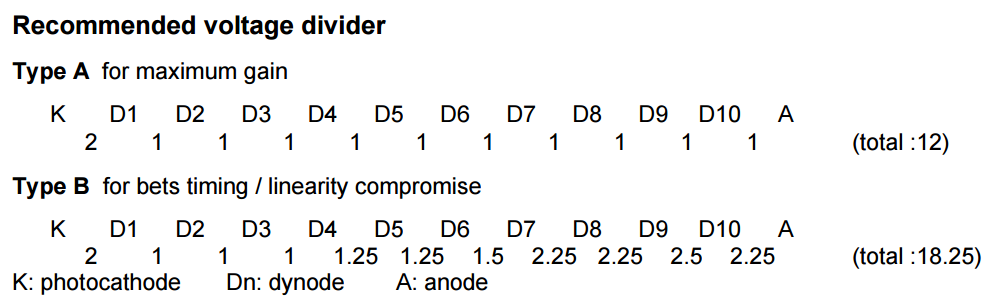
\includegraphics[width=0.7\textwidth]{figures/pmtupgrade/voltage_divider.png}
	\caption{Suggested voltage division schemes for gain vs. timing/linearity compromise~\cite{tubespecs}.}
	\label{fig:voltage_schemes}
\end{figure}

\subsection{Original Base}

The base that came attached to the PMTs were manufactured specifically for use by the ARGUS experiment, which was a relatively (by SeaQuest standards) lower-rate collider experiment that used $e^+ e^-$ annihilation at the \emph{DORIS\ II} ring at DESY. After their tenure at ARGUS, they were handed down to the HERMES experiment located at the \emph{HERA} polarized electron accelerator at DESY.

Though no actual circuit diagram was documented for the original PMT base, it was dissected and each component was measured. The results can be found in Fig.~\ref{fig:original-board}, and its voltage division seen in Fig.~\ref{fig:original-volt}. It features a simple string of resistors with capacitors of increasing capacitance along the last six stages. The voltage division can be recognized to be similar to the timing-linearity compromise scheme described in Fig.~\ref{fig:voltage_schemes}. With a total resistance of approximately \unit[3.95]{$M\Omega$} and the operational voltage of \unit[-1500]{V}, the expected standing (bleeder) current even when sitting in the dark is expected to be \unit[0.38]{mA}. With this in mind, we would expect the voltage divider to destabilize when the signal current approaches this value.

\begin{figure}
	\centerline{
		\mbox{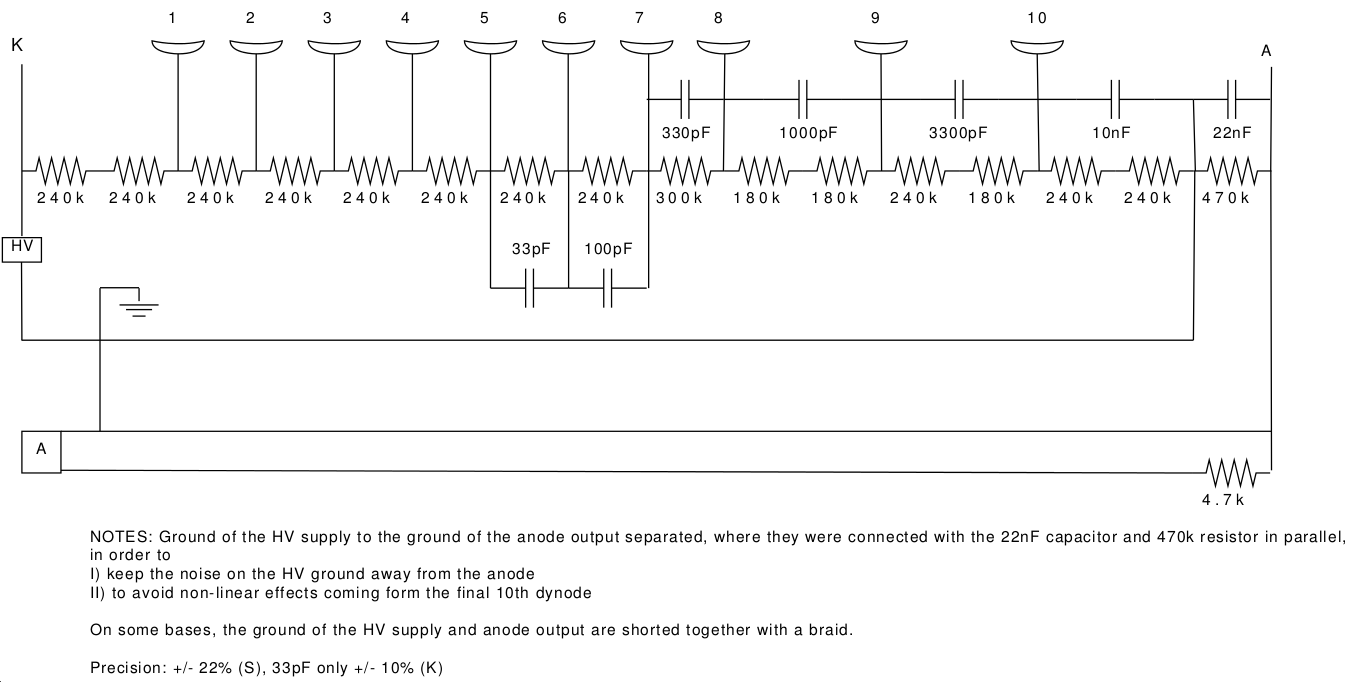
\includegraphics[width=0.75\textwidth]{figures/pmtupgrade/pmt.png}}
	}
	\caption{The original PMT base inherited from the ARGUS and HERMES experiments.}
	\label{fig:original-board}
\end{figure}

\begin{figure}
	\centerline{
		\mbox{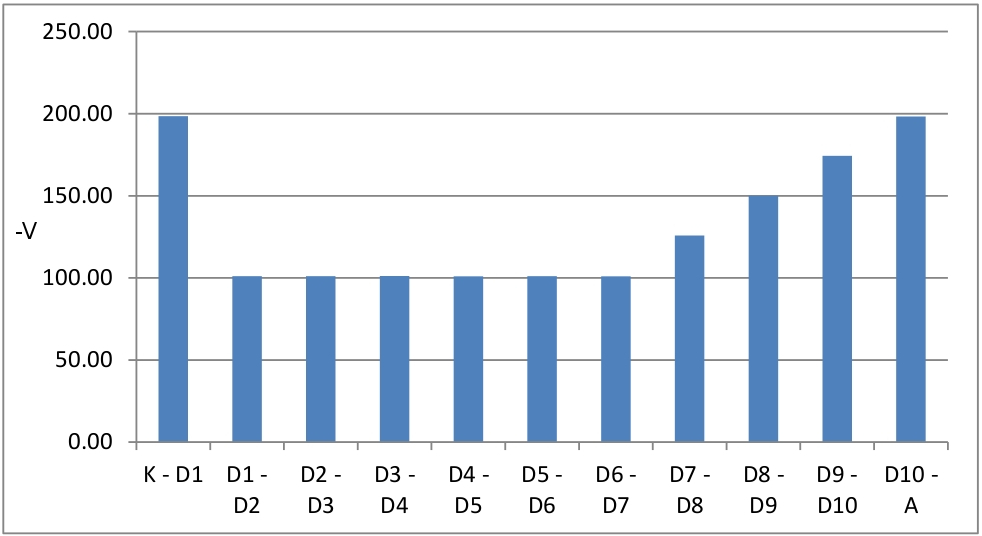
\includegraphics[width=0.55\textwidth]{figures/pmtupgrade/original-volt.jpg}}
	}
	\caption{The voltage division between subsequent stages for the original PMT base design when supplied with \unit[-1500]{V}.}
	\label{fig:original-volt}
\end{figure}

\subsection{Prototype Base v1}

Once the task was set to update the PMT base design, the Fermilab Particle Physics Division was consulted on the matter. In 2010 a base design with similar goals for the exact same PMT model was designed by Sten Hansen~\cite{pc:sten}. The circuit diagram for the new base can be found in Fig.~\ref{fig:v1-board}.

Here, the resistance was significantly reduced by a factor of about 2.9, allowing for much more bleeder current, without exceeding or closely approaching the on-board resistors' power rating. Also, the voltage division was designed to be relatively ``flat'' (Fig.~\ref{fig:v123-volt}) across stages from D1 to A, which is stated to be recommended for optimal gain. With a total resistance of approximately \unit[1365]{$k\Omega$} and the operational voltage of \unit[-1500]{V}, the expected standing (bleeder) current even when sitting in the dark is expected to be \unit[1.1]{mA}. Already here, we see that this design parameter alone suggests its ability to withstand $\sim 3x$ more signal current as compared to the original base.

The introduction of MOSFET transistors is seen between each stage from D7 to D10. Sending the current in parallel over a \unit[1]{$M\Omega$} resistors allows the gate of the transistor to measure the voltage without drawing much current. The Zener dynodes are there in place before each transistor gate to ensure that current only goes one way across the sensitive gate channels.

It is also notable that there are banks of capacitors in parallel across the higher dynode stages. Since there is higher current through this circuit than the original base under the same voltage, there will be a greater demand placed on the capacitors to resupply the dynode stages with spent charge. The two \unit[10]{nF} capacitors in parallel across each stage (which amount to \unit[20]{nF} total) is significantly greater than the capacitance across the stages of the original base.

\begin{figure}
	\centerline{
		\mbox{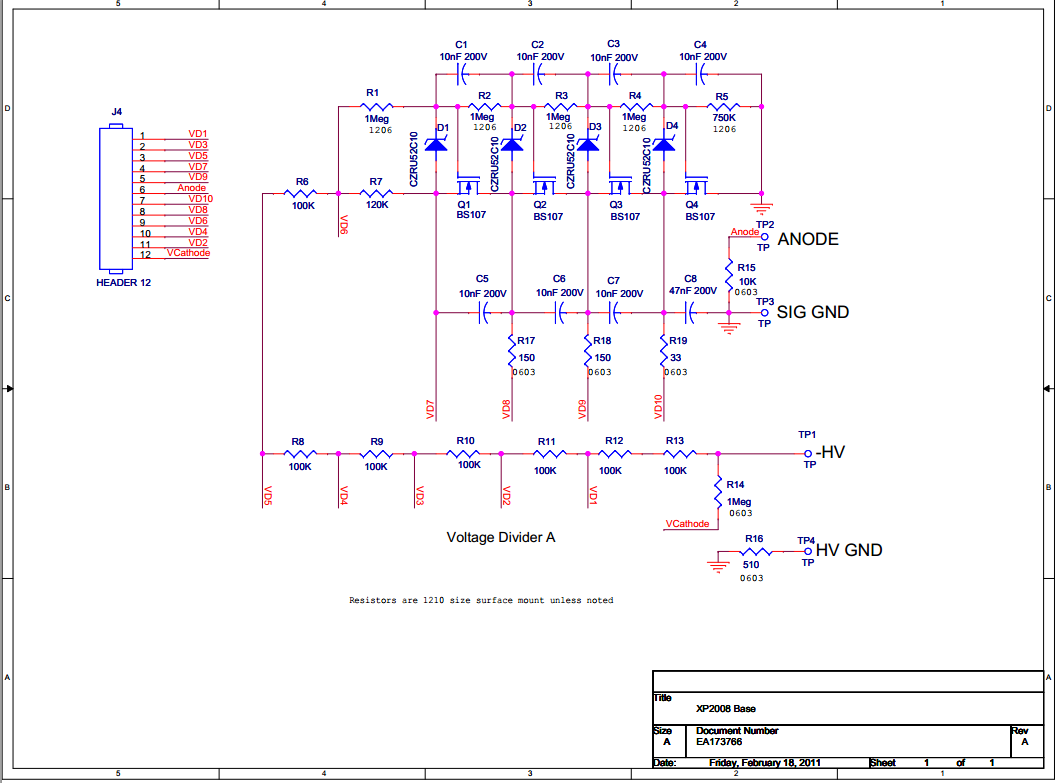
\includegraphics[width=0.7\textwidth]{figures/pmtupgrade/newbase.png}}
	}
	\caption{The Prototype v1 board circuit diagram received from Fermilab Particle Physics Division~\cite{pc:sten}. The parts are denoted as R: resistor, C: capacitor, Q: MOSFET transistor, D: Zener diode.}
	\label{fig:v1-board}
\end{figure}

\begin{figure}
	\centerline{
		\mbox{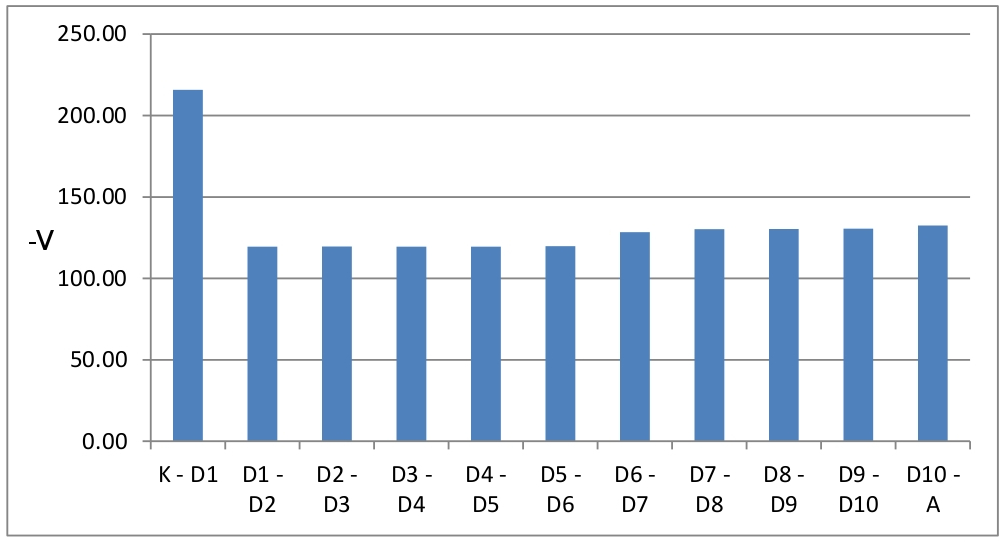
\includegraphics[width=0.55\textwidth]{figures/pmtupgrade/v123-volt.jpg}}
	}
	\caption{The voltage devision between subsequent stages for the Prototypes v1, v2, and v3 PMT base designs  when supplied with \unit[-1500]{V}.}
	\label{fig:v123-volt}
\end{figure}

\subsection{Prototype Base v2}

The first modification made to the prototype board was to keep everything identical except for the total resistance of the circuit. This was accomplished by halving the resistance of each of the first six stages (R6-R13 on Fig.~\ref{fig:v1-board}) from to increase the bleeder current. The resulting current of the base at \unit[-1500]{V} is at around \unit[2.2]{mA}. The voltage division retained the same values as described in Fig.~\ref{fig:v123-volt}.

\begin{figure}[h]
	\centerline{
		\mbox{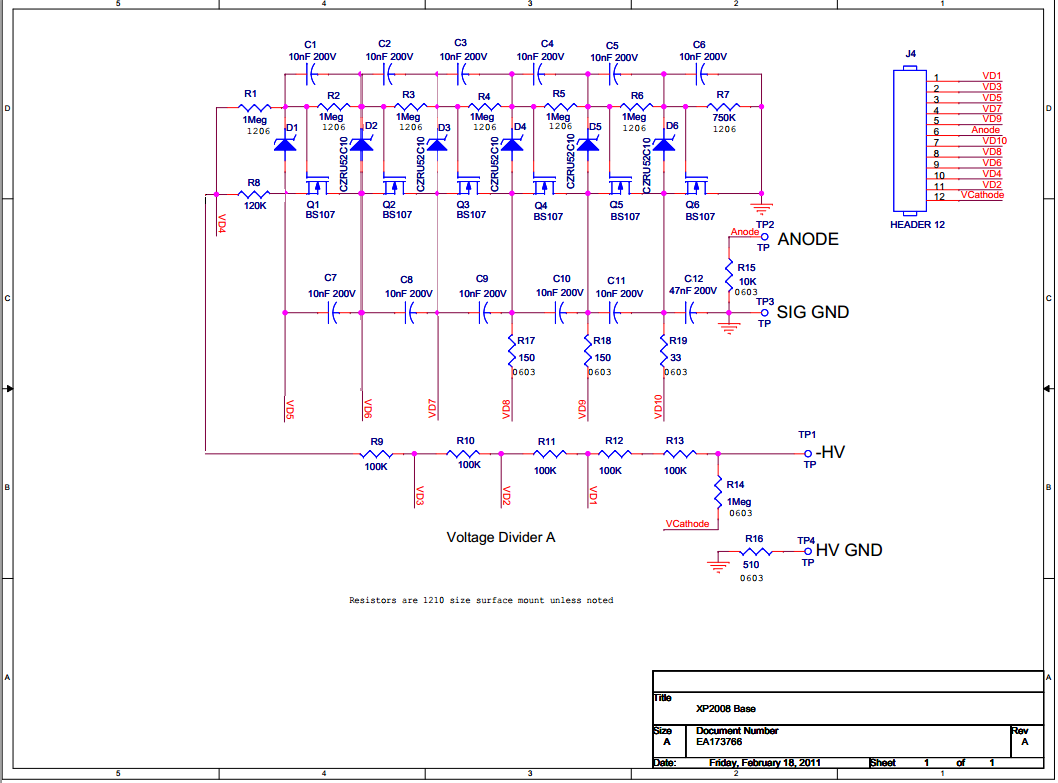
\includegraphics[width=0.7\textwidth]{figures/pmtupgrade/newbase_6mosfet.png}}
	}
	\caption{The Prototype v3 board: 3 more transistorized stages than the Prototype v1 design.}
	\label{fig:v3-board}
\end{figure}

\subsection{Prototype Base v3}

In the case that destabilization was occurring prior to the dynode stages with the added capacitors and transistors, the third prototype was decided to take the Prototype v1 design and add more ``transistorized'' stages earlier on. This entailed extending the parallel configuration of capacitors, transistor, diode, and \unit[1]{$M\Omega$} to the D5-D6 and D6-D7 stages. This prototype configuration can be seen in Fig.~\ref{fig:v3-board}). The voltage division was not significantly altered by this change and remained relatively the same as what is described in Fig.~\ref{fig:v123-volt}.

\subsection{Prototype Base v4}

The final modification arose from a suggestion from a Fermilab collaborator. It was suggested that it may significantly extend the dynamic range of the tube/base by increasing the voltage drop in, specifically, the last stage relative to the other stages.  This reduced to simply replacing R5 (of Fig.~\ref{fig:v1-board}), a \unit[1]{$M\Omega$} resistor, with a \unit[1.5]{$M\Omega$}.  All of the rest would remain unchanged from Prototype v1. The premise for this modification was in the case that the final batch of electrons needed help being ``swept'' to the anode with a higher voltage difference. The change applied resulted in the voltage distribution according to Fig.~\ref{fig:v4-volt}.

\begin{figure}
	\centerline{
		\mbox{\includegraphics[width=0.55\textwidth]{figures/pmtupgrade/v4-volt.jpg}}
	}
	\caption{The (negative) voltage between subsequent stages for the Prototype v4 PMT base.}
	\label{fig:v4-volt}
\end{figure}

\section{PMT Base Comparisons}

There is a specific difficulty with the objective to increase the rate capability of our PMT's. This difficulty is that there was not a known instantaneous intensity or target rate capability to attain. The intensity that caused the original PMT performance to sag is unknown, and if it was known, it would be difficult to match the intensity with an experimental setup. As a result, the objective of these tests was to \emph{compare} the performance of the same PMT under controlled conditions using the original and various prototype bases.

Due to the effects of using different PMTs and due to temperature and humidity fluctuations, the PMT behavior can be somewhat variable from test to test. For this reason, one can only reasonably compare results within each base comparison test, and not across different comparison tests. Each was performed on different days, and sometimes with different PMTs.

\subsection{Testing Apparatus, Measurements, and Procedure}

In this experiment, a PMT attached to a PMT base was placed into a light-tight box facing a fast-pulsing 470nm wavelength LED, which provides the driving photonic signal. 

\subsubsection{PMT Test Setup}

The LED light source assembly consisted of a machined aluminum block that housed the LED, which was a fast-pulsing, narrow beam, water-clear blue LED, peaking in the $\lambda =$\unit[450]{nm} region. This block had a sliding aluminum insert which had a $1/4$'' depression used for inserting a 1'' diameter NDF of arbitrary optical density~\cite{ames1998measurement}. The LED, according to specifications, has a \unit[N]{ns} rise time and a \unit[N]{ns} fall time, which is important when considering pulsing frequencies on the order of \unit[30]{MHz}.

The LED itself was driven by an Agilent 33520 Function / Arbitrary Waveform Generator~\cite{agilent:33520} capable of generating signals up to 30MHz. The LED's unattenuated intensity was far too much light to perform any useful test with such photosensitive hardware. Its intensity was attenuated by use of a neutral density filter (NDF), with a rating $D=3.0$, where the NDF allows 1 in $10^D$ photons through (1 in 1000 for $D=3.0$). When testing began, a $D=4.0$ NDF was used, but the amount of light reaching the PMT was so small that no decrease in PMT performance for any of the bases was observed all the way up to the highest LED frequencies. As such, the $D=3.0$ NDF was chosen for this study.

These were all kept within the light-tight box\footnote{These light-tight boxes are paradoxically referred to as both ``light boxes'' and ``dark boxes'', as they're used for testing \emph{light}-sensitive equipment and they're made to be very \emph{dark} inside.} loaned to the SeaQuest collaboration from the Daya Bay group. This light box was equipped with a patch panel that had both BNC and HVBNC connectors by which to power the PMT base and read out its signal. The light box and all of the installed components can be seen in Fig.~\ref{fig:pmtsetup}.

\begin{figure}
	\centerline{
		\mbox{\includegraphics[width=0.75\textwidth]{figures/pmtupgrade/LightBox.pdf}}
	}
	\caption{Inside of the light box, with the prototype board (left) wired up to a Philips XP-2008 PMT (middle), facing a fast-pulsing LED source (right).}
	\label{fig:pmtsetup}
\end{figure}

A simple data acquisition was assembled from an amplifier, discriminator, and scaler in order to observe that the PMT was functioning properly and firing off at the rate that the LED was set to pulse at.

\subsubsection{Measured and Calculated Quantities}

The PMT base was powered by a high voltage supply, and an ammeter was connected between the two in order to measure the amount of current drawn, or bleeder current, from the HV power supply. The PMT signal was processed by an oscilloscope, averaging the pulse over 300 pulses. The primary measurement was measuring the area of the averaged pulse ($V\cdot s$).

We calculated the signal current from the anode as:
\begin{eqnarray}
Q_{pulse} & = & \frac{\int V dt}{R} \\
I_{signal} & = & f Q_{pulse}
\end{eqnarray}
where $f$ here is the driving frequency of the pulsing LED, $R$ is the termination resistance of the signal (\unit[50]{$\Omega$}), and $\int V dt$ is the integrated area of the averaged PMT pulse. The amplitude of the pulses was also measured, as it was important in determining if it were feasible to remove the typically noisy hodoscope amplifiers from the SeaQuest stations 1 and 2 DAQ setup.

The measured and calculated quantities of interest are the bleeder current, the averaged signal amplitude, averaged signal area, and signal current over the anode.

Due to the limitations of the instruments used in these tests, there is some systematic uncertainty to consider. The ammeter used to measure the bleeder current between the HV supply and the PMT base used an analog gauge that had closely spaced ticks at \unit[0.2]{mA} intervals. As such, the systematic uncertainty for the bleeder current is considered to be $\pm$\unit[0.05]{mA}. Also, due to pulse-to-pulse variations which cause a mild amount of smearing in the average, the measurement of the amplitudes and signal areas have an uncertainty of $\pm$\unit[5]{mV} and $\pm$\unit[0.1]{nVs}, respectively. The uncertainty in the signal area translates to an uncertainty in the calculated signal current of around $\pm$\unit[0.04]{mA}. These fluctuations are considered negligible with respect to the quantities measured.

\subsubsection{Test Procedure}

Most of the prototyping was performed over the span of two weeks. As new suggestions were made at base improvements and the iterations v1-v4 progressed, more comparison tests were performed. The procedure for the each test was the same and is as follows:
\begin{enumerate}[itemsep=-1ex]
	\item Connect the base to the PMT and to the HVBNC and BNC connectors.
	\item Close the lid to the light box.
	\item Gradually power the PMT (\unit[-250]{V} every \unit[5]{s}) until it is as \unit[-1500]{V}.
	\item Watch the scaler counter on the DAQ to see if it is rapidly counting. No (or very few) counts on the scaler. means the box is light-tight.
	\item Let the PMT and base warm up to near-operational temperatures with its standing current for a minute or two.
	\item Power on the function generator and LED, setting the function generator to create a \unit[16]{ns} square wave pulse to the LED circuit (the minimum achievable pulse width~\cite{agilent:33520}) at a frequency of \unit[10]{Hz}.
	\item For each of several frequencies from \unit[10]{Hz} to \unit[30]{MHz}, perform the following:
	\begin{enumerate}[itemsep=-1ex]
		\item Observe the scaler to ensure that the count is increasing at the same rate as is set by the function generator. This confirms that both the PMT, base, function generator, and LED are generally working as planned.
		\item Trigger on the signal from the PMT output.
		\item Average the signal over 300 triggered pulses and then freeze the frame.
		\item Record the current draw from the HV supply (bleeder current).
		\item Measure and record the pulse amplitude with the oscilloscope cursor.
		\item Measure the pulse area using the signal integration feature, setting vertical cursors at the zero-intercept on each side of the pulse.
		\item Return to triggering mode and increase the function generator frequency as warranted.
	\end{enumerate}
	\item Power off the function generator and LED circuit.
	\item Step the PMT voltage down slowly to \unit[0]{V}.
	\item Open the light box and replace the base for subsequent tests as necessary, repeating the steps above.
\end{enumerate}

\subsection{Original vs. Prototype v1}

The first test was to compare the original base with the first iteration of the prototype base. It was generally expected that this new design with more modern technology would exceed the performance of the original base, but the question was twofold: to what extent does it perform better and what is the baseline by which to compare future improvements? 

\begin{figure}[ht]
	\centerline{
		\mbox{\includegraphics[width=0.5\textwidth]{figures/pmtupgrade/Test_v1_Amp.eps} \includegraphics[width=0.5\textwidth]{figures/pmtupgrade/Test_v1_Current.eps}}}
	\caption{Measurements of the (a) signal amplitudes and (b) bleeder and signal currents in the original and prototype v1 PMT bases. The HV was inadvertently set to \unit[-1600V]{V} for this test instead of the intended \unit[-1500]{V}.}
	\label{fig:test-v1}
\end{figure}

The first important observation is the baseline amplitudes of the signals from the two bases, as seen in Fig.~\ref{fig:test-v1}(a). While the absolute voltage itself is not as useful since the LED doesn't necessarily reflect actual operating conditions, we do see that the amplitude from the new base design is increased by a factor of more than two. This in itself is significant in when considering the limits of the discriminators that were used in the hodoscope arrays for Stations 1 and 2. With even a modest boost to gain and signal amplitude, the PMT signals should be large enough that an amplifier is not required in order to get a discriminator to trigger on a PMT pulse. Seeing as the amplifiers used had often caused troubles with the amount of electronic noise they tended to imbue, this was an encouraging observation.

Next, we look at the behavior of the amplitudes as the frequency progresses. It is safe to assume that the unchanging behavior in the lower frequencies indicate that the voltage divider is stable and that there is no voltage breakdown yet. At higher frequencies, there is a qualitative peak in amplitude for both bases, followed by a steep decline. This rise and then sharp fall would seem to indicate the end of stable PMT base operation, with the fall indicating the onset of degradation of performance.

To better identify the conditions that cause this onset, we look to currents applicable to both bases (Fig.~\ref{fig:test-v1}(b)). In this particular test, we see the original base peak in amplitude at $\sim$\unit[4]{MHz} and prototype base v1 peak at $\sim$\unit[10]{MHz}. Looking to the currents, we see that these particular points mark a certain point for both where the signal current reaches almost exactly 50\% of the bleeder current. The baseline improvement with this base over the original one was estimated to extend the operational range by a factor of three -- the point where the amplitude drops below the low-frequency baseline.

Around the time of these tests, Sten Hansen conducted a SPICE (Simulation Program with Integrated Circuit Emphasis) simulation of the prototype circuit and was able to reproduce what was observed. In particular, it was observed that the gain began to change dramatically when the anode (signal) current reaches a significant fraction of the total current drawn from the HV supply; a current that is much less than 100\%. It was concluded that 50\% was consistent with his findings.

\subsection{Original vs. Prototype v1 vs. Prototype v2}

Several suggestions were made in altering the prototype base in order to maximize this improvement, including lowering the overall resistance of the circuit. If the signal current grows at the same pace, then by increasing the bleeder current, there is a chance that a higher frequency signal will be required to bring the signal current up to the point where the divider breaks down, which we estimated above to be $\sim 50\%$ of the increased bleeder current.

\begin{figure}[h]
	\centerline{
		\mbox{\includegraphics[width=0.5\textwidth]{figures/pmtupgrade/Test_v2_Amp.eps} \includegraphics[width=0.5\textwidth]{figures/pmtupgrade/Test_v2_Current.eps}}}
	\caption{Measurements of the (a) signal amplitudes and (b) bleeder and signal currents in the original, prototype v1, and prototype v2 PMT bases.}
	\label{fig:test-v2}
\end{figure}

Looking to Figure~\ref{fig:test-v2}(a), we see that this basic premise is technically sound. The prototype v2 base exceeds the dynamic range of both the original base and the prototype v1 base by factors of approximately a factor of four and two, respectively. This is a significant improvement, and this, at first, seems to be an avenue to pursue. However, an issue arose after increasing the LED frequency from \unit[13]{MHz} to \unit[14]{MHz} when a resistor burned out. The test continued with the rest of the bases, but the results paint a clear picture of what happened. 

By halving the resistance, the bleeder current doubled (Figure~\ref{fig:test-v2}(b)). This caused the power being dissipated by the resistors to exceed their power rating. The prototype bases were built with \unit[0.25]{W} resistors, and as the bleeder current rose well above \unit[2.5]{mA}, one of the resistors failed. This did not bode well for how a smaller on-board resistor might fare with the same current.

To further exacerbate matters, it was found that the LeCroy 1440 HV supplies that were to be used could only supply a maximum of \unit[2.5]{mA} per channel~\cite{lecroy:1440}. Seeing as these power supplies had proven themselves sensitive and prone to communication and performance failures, it was deemed inadvisable to demand anywhere near the maximum current from these HV supplies.

For these reasons, it was decided that the new PMT base design of prototype v1 not be modified in this manner which might suffer from overheating, component failure, and a too-high current demand.

\subsection{Prototype v1 vs. Prototype v3}

Perhaps it was the case that the ``transistorized'' steps were doing their job well and the destabilization was occurring at prior stages. Since the only downside of adding additional steps was added cost, a base with more transistorized stages was created as depicted in Fig.~\ref{fig:v3-board}.

\begin{figure}[h]
	\centerline{
		\mbox{\includegraphics[width=0.5\textwidth]{figures/pmtupgrade/Test_v3_Amp.eps} \includegraphics[width=0.5\textwidth]{figures/pmtupgrade/Test_v3_Current.eps}}}
	\caption{Measurements of the (a) signal amplitudes and (b) bleeder and signal currents in the prototype v1 and prototype v3 PMT bases.}
	\label{fig:test-v3}
\end{figure}

As is quite evident in Figure~\ref{fig:test-v3}, there was no significant difference in the performance of the two prototype bases. As such, this modification was not adopted into the final design.

\subsection{Prototype v1 vs. Prototype v4}

The final test modification of increasing the resistance and thereby the voltage drop across the final D10-A stage was tested against the prototype v1 base.

\begin{figure}[h]
	\centerline{
		\mbox{\includegraphics[width=0.5\textwidth]{figures/pmtupgrade/Test_v4_Amp.eps} \includegraphics[width=0.5\textwidth]{figures/pmtupgrade/Test_v4_Current.eps}}}
	\caption{Measurements of the (a) signal amplitudes and (b) bleeder and signal currents in the prototype v1 and prototype v4 PMT bases.}
	\label{fig:test-v4}
\end{figure}

This modification turns the voltage divider slightly away from the ``optimum gain'' configuration and more towards the ``optimal timing / linearity compromise'' configuration. This is seen to have a direct effect on how a loss in gain can be observed between the v1 and v4 base in Fig.~\ref{fig:test-v4}(a). While the rate capability does seem to slightly increase from \unit[4]{MHz} to \unit[5]{MHz}, the value of having a higher gain was deemed more desirable. Higher gain, again, means that the then-used noisy amplifiers would no longer be needed, and the marginal loss in rate capability was considered a reasonable tradeoff.

\subsection{Base Comparison Conclusions}

After these tests were conducted and the information regarding each of the bases' performances was evaluated, it was decided that the prototype v1 base design was the optimal base configuration to move forward with. This base design yielded a clear improvement in both signal amplitude ($\sim2x$) and rate capability ($\sim3x$) at the expense of more complex circuitry and an increased supply current draw. It then became the task to fit this circuit onto small printed circuit boards (PCBs), and then manufacture, install, and test them.

\section{Base Manufacturing and Installation}

It was decided that the original base structure was well-packaged and well-shielded with its $\mu$-metal canister. As such, a two-component board was designed by Sten Hansen that consisted of a 2.5'' diameter board and a small rectangular ``daughter board''. By June of 2013, the mother and daughter boards (attached) had been manufactured and delivered to UIUC for assembly into the rest of the base.

Since the sockets that coupled the board to the PMT pins was not commercially available, they had to be salvaged by deconstructing the original bases. This consisted of cutting the components between the two boards of the original base and then using a solder vacuum to separate the board from the socket pins. The socket and the other structural elements of the PMT base were separated and prepared for construction with the new base PCB (Fig.~\ref{fig:old-new-base}).

\begin{figure}[h]
	\centerline{
		\mbox{\includegraphics[height=2.5in]{figures/pmtupgrade/disassembled-base.jpg} \includegraphics[height=2.5in]{figures/pmtupgrade/old-new-base.png}}}
	\caption{(Left) The components of the disassembled original base and the manufactured new base PCB with attached daughter board. (Right) The original and new bases fully assembled, side-by-side.}
	\label{fig:old-new-base}
\end{figure}

The deconstruction and re-soldering of the bases took place over the span of about three weeks. Each base was tested to provide the same voltage division across stages and was tested in operation inside the light box apparatus by observing its signal characteristics and the rate of the scaler counting (which should match up with the LED frequency).

After all bases were constructed and tested, the final task was to find the optimal operating voltage for a PMT assembly that would be suitable for detecting minimum ionizing particles passing through a scintillator paddle similar to the ones used at Stations 1 \& 2 at SeaQuest. We also want the minimum possible voltage, as higher voltages correspond to increased noise. This was performed by assembling three stacked scintillator paddles, each  with a PMT attached to their light guide. Their outputs were passed through a discriminator and then to a coincidence unit, which in turn had its output sent to a scaler counter. The top and bottom PMTs were powered to \unit[-1500]{V}, and their coincidences were counted on one channel of the scaler counter. Simultaneously, the middle paddle, set to a variable voltage setting, had its coincidences with the top and bottom paddles counted on the other channel of the scaler counter. The ratio of these two counts ($\epsilon = (triple\ coincidence) / (top-bottom\ coincidence)$) described the efficiency of the middle hodoscope. The voltage of the middle PMT is varied until a plateau in the efficiency is identified and recorded to be the `nominal voltage' of this reference PMT.

All of the constructed PMT bases and the ``reference'' PMT and base were then sent up from UIUC to FNAL to be installed into Stations 1 \& 2 and used for ``gain matching''. The gain matching is done by exposing a scintillator paddle to a $\gamma$-ray source while connected to a PMT and adjusting its voltage until it produces the same signal amplification, or \emph{gain}, as the rest of the PMTs. The original PMT that the rest are matched to is the reference PMT from the previous efficiency study.

Matching the gain is not a simple task, and the typical approach is to take advantage of a physical phenomenon called the Compton Effect occurs in scintillator material when a $\gamma$-ray scatters off of it. Often times, the $\gamma$-ray of energy \emph{E} will not deposit the whole of its energy, but only a portion of it. The spectrum of the photons that scatter off will have energy
\begin{equation}
E' = \frac{E}{1 + \frac{(1-\cos \theta) E}{m_e c^2}}
\end{equation}
where $\theta$ is the angle of deflection and $m_e$ is the electron mass. This, in turn, deposits transferred energy $E_T = E - E'$ into the scintillator which has a maximum value of
\begin{equation}
(E_T)_{max} = E \left( 1 - \frac{1}{1-\frac{2 E}{m_e c^2}} \right)
\end{equation}
This energy is known as the Compton Edge, as it is characterized by a very sharp falloff in the energy spectrum of energy deposited by a source of a specific energy. The particular energy of this edge is not important for the purpose of gain matching. Instead, it's used as a qualitatively sharp feature that can be clearly identified when examining the energy spectrum of photons in scintillator material, as seen in Figure~\ref{fig:cs-137}. As such, it can be used as a landmark to use for adjusting the voltages of each PMT in a way such that the gain of each is the same.

Once installed onto a scintillator paddle, the reference PMT was powered to nominal voltage and a radioactive Cs-137 source was pointed at the paddle. Since the PMT signal has some \emph{linearity} to its signal, the amount of energy of incoming photons will translate approximately linearly to the amount of signal out of the PMT. The signal from the PMT (with the Cesium source pointing at the scintillator paddle) is passed through a qVt (charge-voltage-time) module in ``Q-mode'' to histogram the total integrated charges of the PMT signals. The qVt's channel location of the Compton edge for this reference PMT at this nominal voltage is recorded. Then, every other PMT is powered and measured through the qVt with the Cesium source, and its voltage is adjusted until the Compton edge falls on the same channel. This procedure is generally known as ``gain matching''.

\begin{figure}
	\centerline{
		\mbox{\includegraphics[width=0.75\textwidth]{figures/pmtupgrade/cs-137.pdf}}
	}
	\caption{The $\gamma$-decay energy spectrum of Cs-137 as seen through a scintillator-PMT-qVt setup~\cite{Webb_Williams_1963}. Here, the Compton edge can be seen at channel 110.}
	\label{fig:cs-137}
\end{figure}

\section{New Base Performance}

All of this work is all for naught if the new bases do not hold up to even the highest of beam intensities at SeaQuest. After all of the aforementioned testing, installation, and gain matching, data taking resumed. In Figure~\ref{fig:pmt-high-int}, the hit per event distributions are shown for $x-$ and $y-$measuring hodoscopes as for different intensity ranges. It is difficult to compare these plots to those in Fig.~\ref{fig:sag}, as there was no measure of per-event intensity at the time, and the beam back when that measurement was made was less intense (though just as non-uniform). 
\begin{figure}
	\centering
	\includegraphics[width=0.95\textwidth]{figures/pmtupgrade/final_pmt_dist_vs_int.png}
	\caption{The number of hits per event for the Station 1 hodoscopes for several intensity ranges. Shown is (left) the top $x-$measuring array and (right) the left $y-$measuring array. $I_p$ is in terms of number of incident protons for the event.}
	\label{fig:pmt-high-int}
\end{figure}

Regardless, the new readouts can be interpreted positively. One can see in the $y-$measuring array that the shape does flatten out at the peak for higher intensities. It can be noted that this flattening is much less severe than the ``sag'' that was initially observed. More importantly, when observing the absolute shape of the distribution of the $x-$measuring array, the shape remains intact and uniformly increasing all the way up to the highest intensities. Seeing as the $x-$hodoscopes are the only arrays that are currently being used for triggering and analysis, this is the most important behavior to observe. 

Along with this confirmation, the amplitude output by the PMT signals was above the minimum threshold of the discriminators being used. As a result, the noisy amplifier modules were able to be removed from the signal pipeline and thereby reduced the number of false hits due to electronic noise.
%\chapter{Data Productions}

\section{Production Processing}

The three raw outputs of the data acquisition systems, as described above are (1) Main DAQ CODA files, (2) Scaler DAQ CODA files, and (3) Beam DAQ ASCII files.

Each raw data file corresponds to the data taken from certain subsystems over approximately one to two hours of running time. These three types require varying degrees of de-serialization, parsing, processing, and storage -- a process as a whole defined as \emph{decoding}. 

All raw data files are backed up to long-term tape storage (managed by FNAL Computing Division), and the decoded and processed data gets stored on one of four MySQL servers to be used for analysis by the collaboration. Data is also output to a ROOT file for the ease of use of one of the two independent tracking programs.

Contiguous blocks of decoded and tracked data is then grouped together into \emph{merged} productions, available on all MySQL servers, providing collaborators large sets of curated and easily analyzable data.

\subsection{Decoding Raw Data}

The CODA file decoding is nearly identical for MainDAQ and ScalerDAQ, and only differ by content; the MainDAQ contains TDC readout. For each one to two hour \emph{Run}, the CODA files can be well-described as the following sequence of events (and the data they contain):
\begin{enumerate}
	\item Prestart Event (Run data)
	\item Begin Spill Event (Spill data, Scaler readout)
	\item Many Physics Events (Event data, TDC readout)
	\item End Spill Event (Spill data, Scaler readout)
	\item SlowControl Event (Slow control readout, Spill ID readout)
	\item Spill Counter Event (Spill ID readout) \newline ...(Repeat 2-6 for each \emph{Spill})
	\item End Event
\end{enumerate}

Our decoding program uses C and C++ in conjunction with Jefferson Lab's CODA I/O library to read these events and parse them according to their individual formats. Data from these CODA events are decoded and placed into hierarchical categories.

\subsubsection{Run Level Data}
Run-level data contains data and metadata pertaining to the entirety of the run that is recorded. At the time of the Prestart Event, the date and time of the run are stored, along with a readout of the specific settings of all non-trigger TDC boards.

After the End Event is encountered, metadata is aggregated and stored regarding such items as the number of chamber hits, the triggers that were fired, the target positions used, average magnet currents, and other useful metrics. 

\subsubsection{Spill Level Data}
The \emph{Beginning of Spill} (BOS) and \emph{End of Spill} (EOS) events bookend the set of physics events for a given spill. At each BOS and EOS events, the 140 MHz VME scalers are read out. At the beginning of the spill, all scalers should be zeroed out, and then read out again after the spill has ended.

Slow Control events are read out between spills, which contain data regarding the current spill identifier number, target systems, beam and radiation monitors, and environmental readings.

The spill identifier (\emph{spillID}) is what is used to synchronize the data together across various data acquisition systems. As such, the \emph{spillID} is read out redundantly in both Slow Control and Spill Counter events (which contain only the \emph{spillID} value) to ensure that the data is appropriately labeled.

When the End Event is reached, the independently-recorded Beam DAQ data (recorded in an ASCII file) is read and stored with the rest of the Spill-level data.

\subsubsection{Event Level Data}
For each spill, $\sim3k$ events are triggered to be recorded. With each event, three types of information is stored: the trigger which fired the event, a measure of the beam intensity per RF bucket, and the full detector readouts.
The detector readouts require the most processing of all the rest of the data. The CODA files contain the hardware addresses of each detector \emph{hit}, along with a \emph{TDC time}. The following steps briefly summarize the processing steps:
\begin{enumerate}
	\item Mapping: Map the hardware address to a detector name and detector element number
	\item Timing: Classify hits as in-time or not and calculate \emph{drift time} from TDC time
	\item R-T (time-to-space): Translate \emph{drift time} to \emph{drift distance}
	\item After-Pulse Elimination: Remove hits that result from signal reflection and other electronic artefacts
	\item Trigger Road Reconstruction: Use \emph{v1495} TDC hits to reconstruct possible trigger roads that may have fired
	\item Hodoscope Masking: Remove drift chamber hits that have no adjacent hodoscope hit
	\item Trigger Road Masking: Same as hodoscope masking, but only using hodoscopes from reconstructed trigger roads
\end{enumerate}
This fully processed data is then stored into one the experiment's MySQL databases.

%%%%%%%%%%%%%%%%

\section{Online and Offline Processing}

There are two modes of productions: on-line and off-line productions. For on-line productions, all Run- and Spill-level data is decoded, but only 1-in-$n$ Physics Events are processed, where $n$ is typically $15$. This \emph{``sampling mode''} is used in order for the decoding to reliably keep up with even high-intensity beam data.

For off-line productions, a large group of categorically similar runs is defined, and the chain of production processing is initiated. The steps of this process is generally emph{decoding, tracking, archiving, and merging}.

The decoding and tracking is performed on Fermilab Computing Service's FermiGrid, which provides the computing resources necessary to process hundreds of runs simultaneously.

A single decoding job submission will output the processed data to one of the four available MySQL servers and also to a ROOT file. Then, one job will be submitted to run one of the two tracking programs on the ROOT file, while another job is submitted to run the other tracking program on the MySQL data.

Once the tracking is completed, the ROOT file and the \emph{Hit} table from the MySQL production is archived on the Fermilab BlueArc NAS backup system for future use, if necessary.

Upon the completion of decoding and tracking of a specified range of runs, all of their Run-, Spill-, and Event-level data, along with its tracked data, is combined into a single \emph{merged} schema. These \emph{merged} schemas are mirrored across all four of the MySQL servers for optimal redundancy and availability.

\section{RDBMS Data Structure}

The processed data is primarily stored in MySQL Server 5.1 databases. MySQL is an open-source \textbf{R}elational \textbf{D}ata\textbf{b}ase \textbf{M}anagement \textbf{S}ystem (RDBMS) developed by Oracle that is well-suited for the storage and responsive querying of hierarchical data.

Each run is decoded into its own schema, and contains its own instances of all tables of a specified design. The tables are all \emph{join}-able to each other by sharing \emph{foreign keys} with each other in the form of the \emph{runID}'s, \emph{spillID}'s, and \emph{eventID}'s. The contents of the tables are \emph{indexed} in such a way that \emph{joins} and queries gain a speed performance boost, but this comes at the cost of disk space.

The data on the server is world-wide accessible and can be queried using the standard querying language. The queried data can be directed to any analysis code in any programming language due to the large array of MySQL API's available.

\section{Data Quality}


\chapter{Analysis}

\red{CHAPTER STATUS: PLANNING/OUTLINE}


\section{Reconstruction and Tracking of SeaQuest Dimuons}

\subsection{Hit Reduction}

\subsection{Particle ID}

\subsection{Muon Momentum Reconstruction}

\subsection{Kalman Filter Track Fitting}

\subsection{Vertex Fitting}

\subsection{Monte Carlo Validation}

\section{Data Selection}

\red{Talk about roadset characteristics, amount of data}

\section{Analysis Cuts}

\red{Here give summary of all levels of implemented cuts.}

\subsection{Run Level Cuts}

\red{Give ranges of runs that are excluded. Maybe add a subsection about the manual target position study.}

\subsection{Spill Level Cuts}

\red{Dump out Kenichi's data quality slides here, with some plots showing visualizations of good and bad value ranges for some interesting fields.}

\subsection{Event Level Cuts}

\red{FPGA1 cut and maybe nonsense RF+00 cuts? Should be a brief section.}

\subsection{Dimuon Level Cuts}

\red{x1, x2, xF, mass, trackSeparation, etc.}

\subsection{Track Level Cuts}

\red{Talk about target-dump separation along with the rest of the other cuts.}

\section{Dimuon Yields}

\subsection{Binning of Data}

The $x_2$ bins for this EMC ratio measurement were chosen such that each
bin in $x_2$ has similar levels of statistics. 

Concurrent with this analysis, studies of $\bar{d}(x_2)/\bar{u}(x_2)$ and 
parton energy loss are conducted. Due to the nearly
identical source of signal across these studies (good Drell-Yan target
dimuons), a consistent selection of kinematic binning maintains a 
certain continuity among analyses. The $x_2$ binning chosen can be found in Table \ref{tab:x2bins}

\begin{table}
	\centering
	\setlength\tabcolsep{4pt}
\begin{minipage}{0.48\textwidth}
	\centering
	\begin{tabular}{ll}
		\toprule
		Bin\# & $x_2$ Range\\
		\midrule
		0 & (0.08, 0.14] \\
		1 & (0.14, 0.16] \\
		2 & (0.16, 0.18] \\
		3 & (0.18, 0.21] \\
		4 & (0.21, 0.25] \\
		5 & (0.25, 0.31] \\
		6 & (0.31, 0.53] \\
		\bottomrule
	\end{tabular}
	\caption{$x_2$ bin ranges}
	\label{tab:x2bins} 
\end{minipage}%
\hfill
\begin{minipage}{0.48\textwidth}
	\centering
	\begin{tabular}{ll}
		\toprule
		target & yield \\ 
		\midrule
		None   &  104 \\
		Empty  &  84 \\
		LH2    &  3138 \\
		LD2    &  3472 \\
		C      &  1721 \\ 
		Fe     &  1370 \\
		W      &  1553 \\
		\bottomrule
	\end{tabular}
	\caption{Raw dimuon yields for Roadset 57} 
	\label{tab:targyields} 
\end{minipage}
\end{table}

\subsection{Raw Yields}

\red{Summarize the raw, unweighted and uncorrected yields here.}

\subsection{Live Proton Calculation and Integration}

\red{Summarize the reasoning for the live proton value and define its calculation. Finish with the number of live protons per roadset per target, and then the yields per live proton values.}

\section{Dimuon Weights and Corrections}

Weighting of events is a standard procedure for mapping one distribution onto another. The most common example is with Monte Carlo (MC) simulation weighting. A simple physics event MC meant to simulate a well-defined process will `throw' an event with certain kinematics randomly drawn from known distributions via \emph{inverse transform sampling}. By doing this, the simulation is already close to being physical, but according to the cross section of a given process, a certain combination of kinematics will be decidedly more or less probable. A weighting subroutine calculates this likelihood for each event and assigns a weight with respect to how likely that event is based on the kinematics thrown. When binning this weighted data, the adjusted number of events in a bin is given by
\begin{equation}
	N_{bin} = \sum_{i \in bin} w_i\ \ ;\ \ \sigma_{bin} = \sqrt{\sum_{i\in bin} w_i^2}
	\label{eq:gmc-weight}
\end{equation}
which reduces to the Poissonian statistical picture when all weights are 1.

Weighting in this manner can be used in any case where it is desirable to map one distribution to another, as in the case of applying corrections in the case of efficiencies and background subtractions. The most intuitive connection between the use of weights and corrections is in the case of efficiency corrections. Let us say that a dimuon with a certain set of kinematics, for whatever combination of effects, has a reconstruction efficiency of 80\%. This means that four out of five actual dimuons with these kinematics will be reconstructed. If you know this efficiency $\epsilon_{recon}$, you can apply a weight as $w = 1/\epsilon_{recon}$ to each dimuon, as each dimuon represents, in part, a larger population that is not fully represented. In the case of our example, a single dimuon represents $1/0.80 = 1.25$ dimuons in order to make up for the ones that are missed due to that specific inefficiency.

At SeaQuest, there is an issue of rate dependence, and as the sources of this effect is identified, we apply a correction for each source in the form of an applied weight. Here, we discuss the reconstruction efficiency and empty/none target background subtraction corrections.

\subsection{``kEfficiency'' Correction Using Messy/Clean Data}

It is a matter of combinatorics at SeaQuest that, as the intensity increases, the number of background hits on all of the detectors increases. As the number of hits in all the detectors increases, the harder it become for the tracking to identify the actual dimuon(s) from the whole event. This is regarded to be an intensity-dependent tracking efficiency. Seeing as the primary tracking algorithm for SeaQuest is kTracker, this is known as the ``kEfficiency'', and its intensity, target, and kinematic dependency makes it a factor to model and correct for.

The procedure developed by Evan McClellan of UIUC for calculating this kEfficiency is to take compare the performance of the tracking on a clean MC sample of dimuons to an analogous sample that's mixed in with real intensity-dependent background. To do this, a \emph{single} sample of MC-generated dimuons and all of their hits is generated; this sample is denoted as the \emph{``clean''} sample. Then, this sample is mixed with all of the hits from a NIM3 event from the experimental data. The NIM3 trigger, as is discussed in Chapter~2, is the randoms trigger, and by using these events we avoid any effects due to trigger selection bias. This mix of MC dimuons and NIM3 triggered data is denoted as the \emph{``messy''} sample. These NIM3 events all have an intensity, and by embedding a clean MC dimuon into a situation typical of an event at a given intensity, we get a basis by which to judge how efficiently the tracking can reconstruct a dimuon in the clean sample versus the messy sample as a function of intensity (and other kinematic variable).

It is important to note that the DY cross section is so small that there is a negligible chance that a given randomly-triggered NIM3 event will contain an actual dimuon, nonetheless a dimuon matching the characteristics of the MC dimuon that is embedded. As such, it is assumed that the dimuon embedded in the NIM3 event is the only dimuon to find in the event. It is also justified to assume that the kinematics of a dimuon is in no way correlated to the intensity, and the intensity of an event relates only to the amount of background hits observed. The relation to the intensity and the number of background hits can be observed in Figure~\ref{fig:NIM3-Int-Mult}.

\begin{figure}
	\centering
	\includegraphics[width=4in]{figures/analysis/NIM3-Int-Mult.png}
	\caption{The linear tendency of detector multiplicity to increase with intensity is observed by looking to unbiased NIM3 events. Here, the occupancy per event of the drift chambers at station 2 are shown as a function of intensity.}
	\label{fig:NIM3-Int-Mult}
\end{figure}

Once the messy and clean samples are prepared, the tracking software is run on them and the two outputs are compared. The first step is to bin the resulting reconstructed dimuons into intensity bins. This binning uses the weights of the dimuons that is assigned by the GMC that created them. The weights are used instead to avoid undue influence on the efficiency from dimuons that are highly unlikely to occur. The value of the bin and its uncertainty are calculated according to Eq.~\ref{eq:gmc-weight}.

For each matching bin, the ratio of $\frac{\#messy}{\#clean}$ values is used to calculate the efficiency of the tracking for that bin. The uncertainty of that efficiency is more complicated, as the relation between the messy and clean samples is of a \emph{binomial} nature. Each dimuon successfully reconstructed in the messy sample represents a \emph{positive} outcome from the number of possible outcomes which is represented by the clean sample. With this kind of relationship, binomial uncertainty calculations must apply. For large enough N number of trials and efficiency $\epsilon\notin \{0,1\}$,
\begin{equation}
\epsilon = \frac{N_+}{N}\ \ ;\ \ \delta\epsilon = \sqrt{\frac{N_+ N_-}{N^3}} = \sqrt{\frac{\epsilon(1-\epsilon)}{N}}
\label{eq:binomial-naive}
\end{equation}
but when weighted trials are involved, things become more complicated in calculating the statistical error. The calculation of this statistical error\cite{blist:binomial} is as follows:
\begin{eqnarray}
	\epsilon & = & \frac{\sum\limits_{i\in+}w_i}{\sum\limits_i w_i} \\
	\delta\epsilon & = & \frac{\sqrt{\sum\limits_{i\in+} w_i^2 \left(\sum\limits_{i\in-} w_i \right)^2 + \
			\sum\limits_{i\in-} w_i^2 \left(\sum\limits_{i\in+} w_i \right)^2}} {\left(\sum\limits_{i}w_i\right)^2}
	\label{eq:binomial-weighted}
\end{eqnarray}
where
\begin{eqnarray}
\sum\limits_{i\in-} w_i & = & \sum\limits_{i\in+}w_i - \sum\limits_{i\in+}w_i \\
\sum\limits_{i\in-} w_i^2 & = & \sum\limits_{i\in+}w_i^2 - \sum\limits_{i\in+}w_i^2 
\end{eqnarray}

For a set of efficiencies, a linear function is fit to the efficiencies. This fit function would then be used to calculate the efficiency for any given dimuon that occurs at any given intensity. The linear parameters are fitted to the data (which is weighted by its statistical uncertainties) by a $\chi^2$-minimization procedure to render a line of best fit along with a confidence interval (Fig.~\ref{fig:keff-all})

\begin{figure}
	\centering
	\includegraphics[width=4in]{figures/analysis/all-keff-int.png}
	\caption{The ratio of ``messy'' to ``clean'' dimuon samples from the Deuterium target in Roadset 67 data. This shows the linear relationship of the tracking efficiency to the intensity of the events. The shaded band indicates the 95\% confidence band of the fit.}
	\label{fig:keff-all}
\end{figure}

Further, these fits have a statistically significant kinematic dependence, so it becomes important to unfold the kinematic space and perform this procedure for several kinematic bins in one or more dimensions to assure an accurate efficiency calculation. Of the six defining kinematics of the dimuon, we examine the dependence of the fit on five of them: ($x_1, x_2, p_T, \theta, \phi$), neglecting the azimuthal production angle $\phi_{\gamma^*}$. Each of these five kinematics is divided into three bins (low, medium, high) values to observe on which kinematics the linear fit depends. The results are shown in Figure~\ref{fig:keff-all-kin}.
\begin{figure}
\centering
\includegraphics[width=0.49\textwidth]{figures/analysis/x1-keff-int.png}
\includegraphics[width=0.49\textwidth]{figures/analysis/x2-keff-int.png} \\ \vspace{20px}
\includegraphics[width=0.49\textwidth]{figures/analysis/theta-keff-int.png}
\includegraphics[width=0.49\textwidth]{figures/analysis/phi-keff-int.png} \\ \vspace{20px}
\includegraphics[width=0.49\textwidth]{figures/analysis/pt-keff-int.png} \vspace{10px}
\caption{Tracking efficiency with the data broken into three statistically equivalent bins in the five primary kinematics, ($x_1, x_2, \theta_\mu, \phi_\mu, p_T$). There appears to be a significant kinematic dependence on $x_1$ and $x_2$.}
\label{fig:keff-all-kin}
\end{figure}
The curves produced seem to indicate that there only exists a kinematic dependence on the $x_1$ and $x_2$ kinematics. If this is the case, then the clean and messy samples can be split two-dimensionally in these two kinematics, and a fit can be made to both variables. When analyzing dimuons, its kinematics can indicate which fit to use to calculate the tracking efficiency based on the intensity of the event, and a weight can be calculated.

But before we come to any clear conclusions, let us investigate two more kinematic phase spaces. We know from the discussion in Chapter 1 that \{$x_1, x_2$\} can be used almost interchangeably with \{$x_F, M_{\gamma^*}$\}, and each of $x_1$ and $x_2$ depend on both $x_F$ and $M_{\gamma^*}$. As such, if only one and not the other shows to influence the tracking efficiency curves, then only that one would be needed for the tracking efficiency correction. We see the behavior of the efficiency curves as a function of $x_F$ and $M_{\gamma^*}$ in Figure~\ref{fig:keff-mass-xf}. It can be concluded that since there is no substantial mass dependence observed, the tracking efficiency has a kinematic dependence solely on $x_F$.

\begin{figure}
	\centering
	\includegraphics[width=0.49\textwidth]{figures/analysis/xF-keff-int.png}
	\includegraphics[width=0.49\textwidth]{figures/analysis/mass-keff-int.png}
	\caption{The kinematics $x_F$ and $M_{\gamma^*}$ are investigated. A clear kinematic dependence exists in $x_F$ while $M_{\gamma^*}$ is largely consistent.}
	\label{fig:keff-mass-xf}
\end{figure}

Another consideration is with respect to whether or not there is a target dependence to factor into the correction. For all of the above ``kEfficiency'' plots, only deuterium data is used. The kEfficiency curves for deuterium, hydrogen, carbon, iron, and tungsten can be found on Figure~\ref{fig:keff-target-roadset}. It can be concluded that there is enough of a difference between deuterium, iron, and the rest to justify calculating and applying this correction on a target-by-target basis.
\begin{figure}
	\centering
	\includegraphics[width=0.49\textwidth]{figures/analysis/target-keff-int.png}
	\includegraphics[width=0.49\textwidth]{figures/analysis/roadset-keff-int.png}
	\caption{Comparing the tracking efficiency curves across (left) the five targets and (right) two temporally different subsets (different roadsets) of data. Confidence bands removed from the target plot for the sake of clarity.}
	\label{fig:keff-target-roadset}
\end{figure}

Also, as a sanity check, there should be no time-dependence of this function. A quick check comparing different sets of data from two different roadsets quickly confirm that there is no such time dependence (Fig.~\ref{fig:keff-target-roadset}).

As a result, the final calculation of an tracking efficiency for a given dimuon event should depend on (1) target, (2) $x_F$, and (3) intensity. In order to apply this as a weight, we first define \emph{kEff}$_{t, \bar{x}}(I)$, a set of linear fit functions: one for each target (\emph{t}) and for each kinematic bin ($\bar{x}$), which may be binned in any number of kinematic dimensions. In the case of this analysis, the kinematic binning will only be in $x_F$. The procedure in weighting each dimuon will then be to take each dimuon event \emph{i} and its chamber intensity $I_i$, originating from target $t_i$ in $x_F$ bin $x_{F_i}$, create a weight as
\begin{equation}
w_i = \frac{1}{kEff_{t_i, x_{F_i}}(I_i)}
\end{equation}

\subsection{The Naive Empty/None Correction}

First a few values must be defined. An overall efficiency based on 'contributions' from the Empty/None background can be defined as

\begin{equation}
\epsilon_b = 1 - \frac{Y_b/p_b}{Y_t/p_t} = 1 - \left(\frac{p_t}{p_b}\right) \left( \frac{Y_b}{Y_t} \right)
\end{equation}

where Y is the dimuon \emph{yield} from a given target and \emph{p} is the integrated ``live proton'' count for the same given target. Here, $b \in \{Empty,\ None\}$ and $t\in\{H,\ D,\ C,\ Fe,\ W\}$. It is yet to be conclusively decided by the collaboration whether or not the Empty and None targets are to be combined for these calculations.

The next step is to adjust the yields with the \emph{kEff}$_{t,\bar{x}}(I)$:

\begin{equation}
Y_a \rightarrow Y_a^\prime = \sum_{i:i_t=a} \frac{1}{kEff_{t_i, x_i}(I_i)}
\end{equation}

The yield efficiency when factoring in background then becomes

\begin{equation}
\epsilon^\prime_b = 1 - \left(\frac{p_t}{p_b}\right) \left( \frac{Y^\prime_b}{Y^\prime_t} \right)
\end{equation}

\subsection{The Empty/None vs. Intensity Curve}


\subsection{Improved Background Correction}

With the Empty/None vs. Intensity Curve \emph{C(I)}, we can apply a more sophisticated correction. With C(I), we can make an expression for the background contribution to the yields of a given target:

\begin{equation}
p_t \left( \frac{Y^\prime_b}{p_b} \right) = \sum_{i:i_t=t} \frac{D\cdot C(I_i)}{kEff_{t_i, x_i}(I_i)}
\end{equation}
where D is a normalization constant defined in such a way that $D \cdot C(I)$ is the \% chance that a given dimuon from a target actually came from the Empty/None background. D can be calculated as
\begin{eqnarray}
D & = & \frac{1}{F} Y^\prime_b \left( \frac{p_t}{p_b} \right) \\
F & = &\sum_{i: i_t=t} \frac{C(I_i)}{kEff_{t_i, x_i}(I_i)}
\end{eqnarray}

The new intensity-dependent efficiency can now be defined as

\begin{equation}
(\epsilon_b^\prime)_i = 1 - D \cdot C(I_i)
\end{equation}

\section{Combinatorial Background Correction}

\red{Discuss analysis investigating results for the like-sign reconstruction to estimate the combinatorial background. Hopefully it will be intensity-dependent.}

\section{$ld_2$ Contamination Correction}

\red{Discuss contamination backstory, composition breakdown, the fluctuation from bottle-to-bottle, the correction procedure, and the proposed systematic uncertainty in that procedure.}

\section{Isoscalar Corrections for $^{183}W$ and $^{56}Fe$}

\red{Give brief correction in approximating n==p conversion. Be sure to show results for both iso-corrected and not!}


\chapter{Results}

\red{CHAPTER STATUS: NOT STARTED}

\section{Dimuon Yield Ratios}

\red{Give EMC ratios, maybe parton energy loss ratios. If there's time, maybe quarkonia ratios. Show for separate roadsets and with/without corrections. Show heavy-to-heavy ratios, too.}
\chapter{Discussion}

\red{CHAPTER STATUS: NOT STARTED}

\chapter{Conclusions}

We conclude that Bryan Dannowitz likes coffee.


\appendix


\chapter{PMT Upgrades}

\section{ARGUS PMT Performance 'Sag'}

\section{Prototype Testing}

\section{Manufacturing and Installation}

\chapter{MySQL Production Structure}

\section{MySQL Servers}

\section{Atomic Schema Design}

\section{Merged Schemas}
	


\backmatter

\bibliography{thesisbib}
\bibliographystyle{plain}

\end{document}
\endinput
%%
